% --------------------------------------------------------------------------- %
% --------------------------------------------------------------------------- %
\chapter{Background Estimation Methods}
\label {ch:bkgd}
% --------------------------------------------------------------------------- %
% --------------------------------------------------------------------------- %
The techniques used to estimate the SM backgrounds in the signal regions are descibed in detail in this chapter.
The SM backgrounds fall into three categories, Z+jets, Flavor symmetric, and other SM backgrounds.
The first two backgrounds are estimated using a data-driven method developed for this analysis,
and the backgrounds falling into the third category are estimated using MC simulation.
The MC samples used to estimate these backgrounds are studied in a control region which is orthogonal to the signal regions.

\section{Estimating the \texorpdfstring{\zjets}{Z+jets}\ Background with \texorpdfstring{\MET}{MET}\ Template}
\label{sec:bkg_zjets}
The \zjets\ background is estimated using a method named the \MET\ template method.
The estimate is done using a control sample of data events gathered using a suite of single photon triggers.
In events with a Z boson recoiling off of a system of jets, there should be no real \MET.
However, the resolution of the jet system is poor leading to events with \MET\ due to these effects.
The resolution of photons is similar to that of leptons,
so the assumption is made that \MET\ in \gjets\ events is from the same sources as in \zjets\ events.
This method also works in cases where there is real \MET\ in the event,
for example when an event containing a b-jet that decays semi-leptonically,
since the \MET\ source is not from the leptons or photon.
The main difference between these samples is the fact that the Z-boson is massive whereas the photon is not.
To account for this difference,
the photon's \pt\ distribution is reweighted to match that of the dilepton system's \pt.

This method does not require that the photon-like object used in the \gjets\ events be extremely pure,
it only matters that the photon-like object is well-measured.
The selection described in Sec.~\ref{ssec:phosel} is used to select the photon-like object.
The \gjets\ events are selected with a suite of single photon triggers with \pt\ thresholds varying from 22--165 GeV.
These triggers as well as their average prescales are listed in table~\ref{tab:photontriggers}.
Each \gjets\ event is weighted by the trigger prescale, such that these events evenly sample the conditions over the full 2015 year period of data taking.
When an event passes a trigger, the trigger information is stored for all triggers that pass.
Due to the way the prescale software is written,
the triggers with larger prescales must be prescaled by an integer multiple of a lower prescale value,
otherwise the trigger information will not be saved.

\begin{table}[htb]
  \begin{center}
    \caption{
      \label{tab:photontriggers}
      List of single photon triggers used in this analysis and their prescales.
    }
    \begin{tabular}{l|l|l}
      \hline
      \hline
      \pt\ threshold [\gev] & trigger name                               & prescale \\
      \hline
      22                    & \verb=HLT_Photon22_R9Id90_HE10_IsoM_v*=  & 1008 \\ 
      30                    & \verb=HLT_Photon30_R9Id90_HE10_IsoM_v*=  &  504 \\
      36                    & \verb=HLT_Photon36_R9Id90_HE10_IsoM_v*=  &  168 \\
      50                    & \verb=HLT_Photon50_R9Id90_HE10_IsoM_v*=  &   24 \\
      75                    & \verb=HLT_Photon75_R9Id90_HE10_IsoM_v*=  &    4 \\
      90                    & \verb=HLT_Photon90_R9Id90_HE10_IsoM_v*=  &    2 \\
      120                   & \verb=HLT_Photon120_R9Id90_HE10_IsoM_v*= &    1 \\
      165                   & \verb=HLT_Photon165_R9Id90_HE10_IsoM_v*= &    1 \\
      165                   & \verb=HLT_Photon165_HE10_v*=             &    1 \\
      \hline
      \hline
    \end{tabular}
  \end{center}
\end{table}

In order to account for the fact that the Z-boson is massive wheras the photon is massless, 
the \gjets\ sample is reweighted such that the boson \pt\ matches that of the \zjets\ sample.
A separate reweighting scheme is derived for each signal region, where the same cuts on $\mathrm{N_{jets}}$\ and \HT\ are applied to the \zjets\ and \gjets\ data samples.
The result of this reweighting can be seen in figures~\ref{fig:photonptreweighting} and~\ref{fig:metptreweighting}.

\begin{figure}[!htb]
  \begin{center}
    \begin{tabular}{cc}
      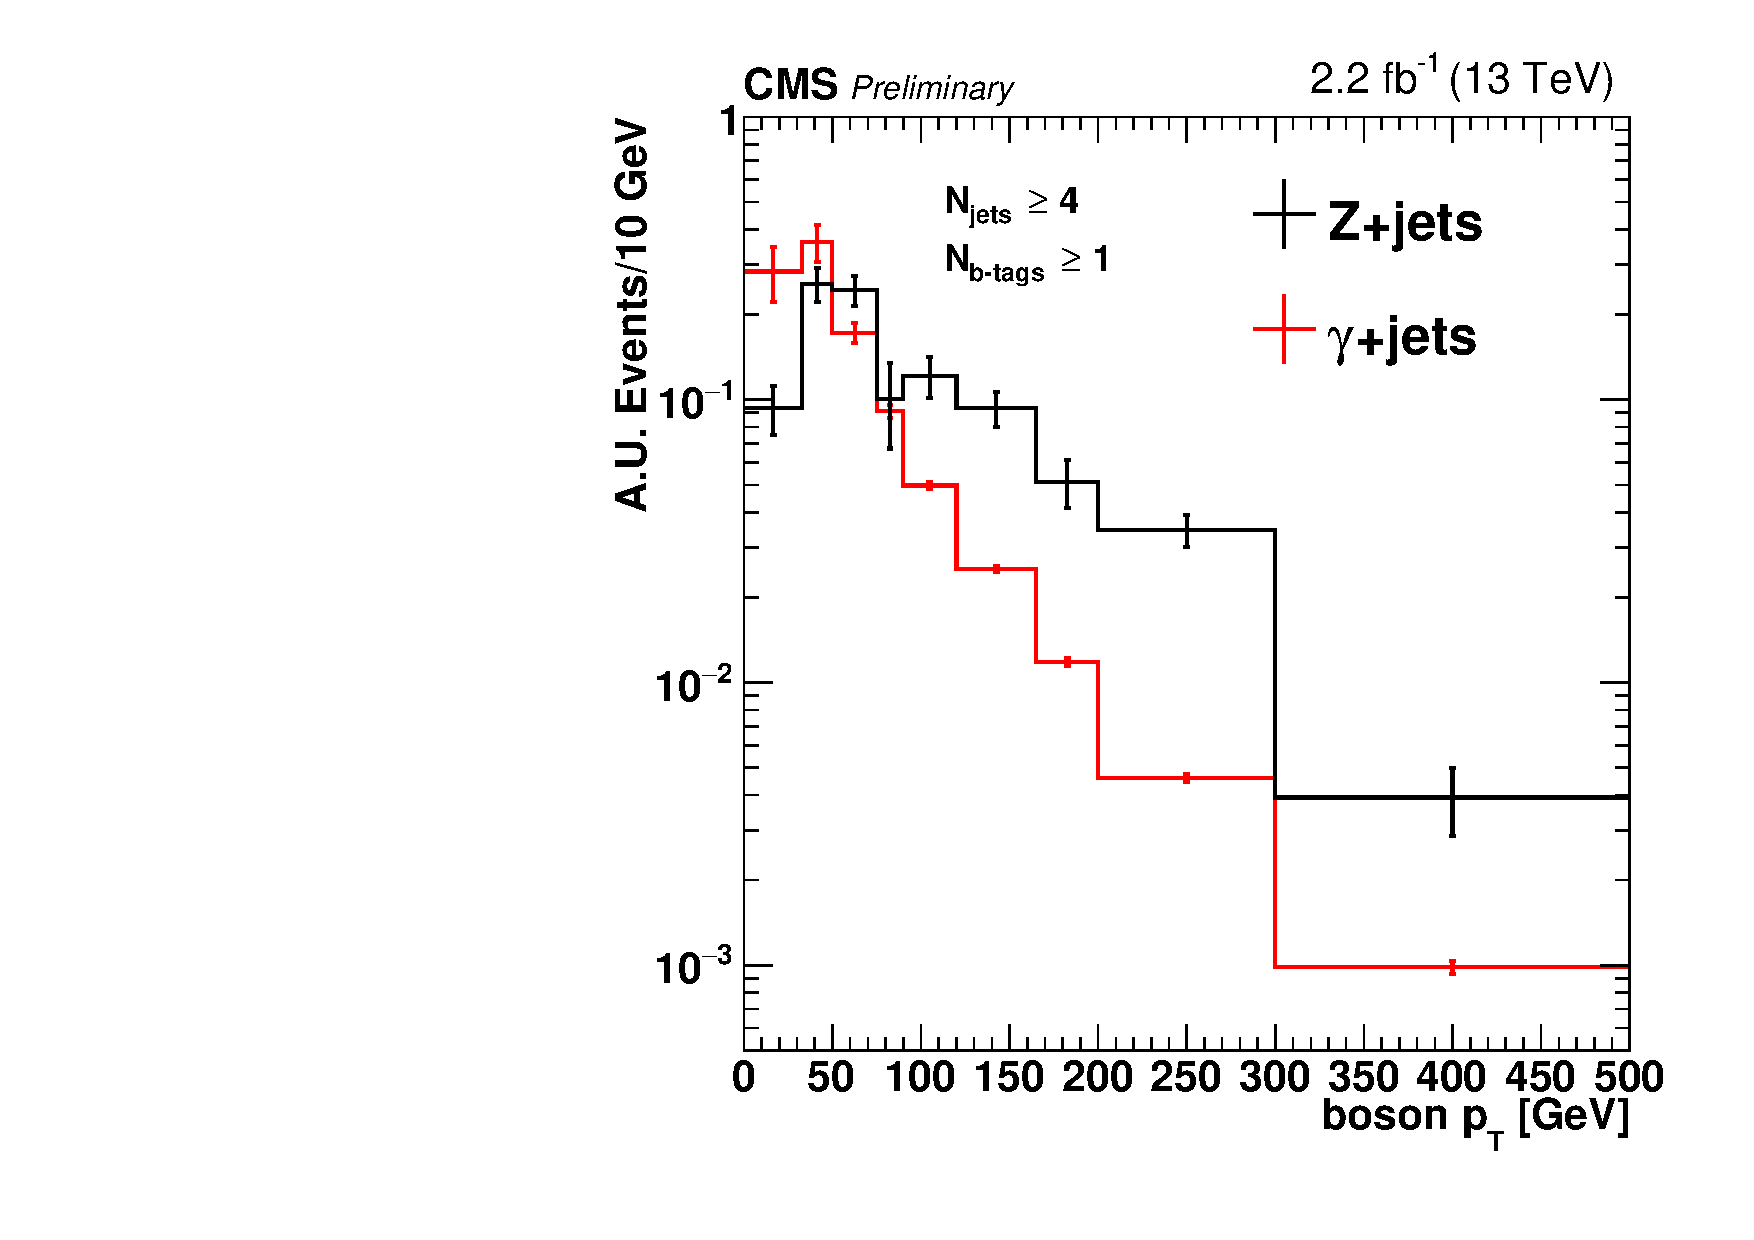
\includegraphics[width=0.8\textwidth]{bkgd/figs/photon_SRB_2p1fb_vs_dilep_ptg_withb.pdf}
    \end{tabular}
    \caption{
      The \pt\ distributions are shown for the \zjets\ (black) and \gjets\ (red) events
      in signal region B where at least 1 jet is required to be b-tagged.
      The distributions are normalized to unit area.
      \label{fig:photonptreweighting}
    }
  \end{center}
\end{figure}

\begin{figure}[!htb]
  \begin{center}
    \begin{tabular}{cc}
      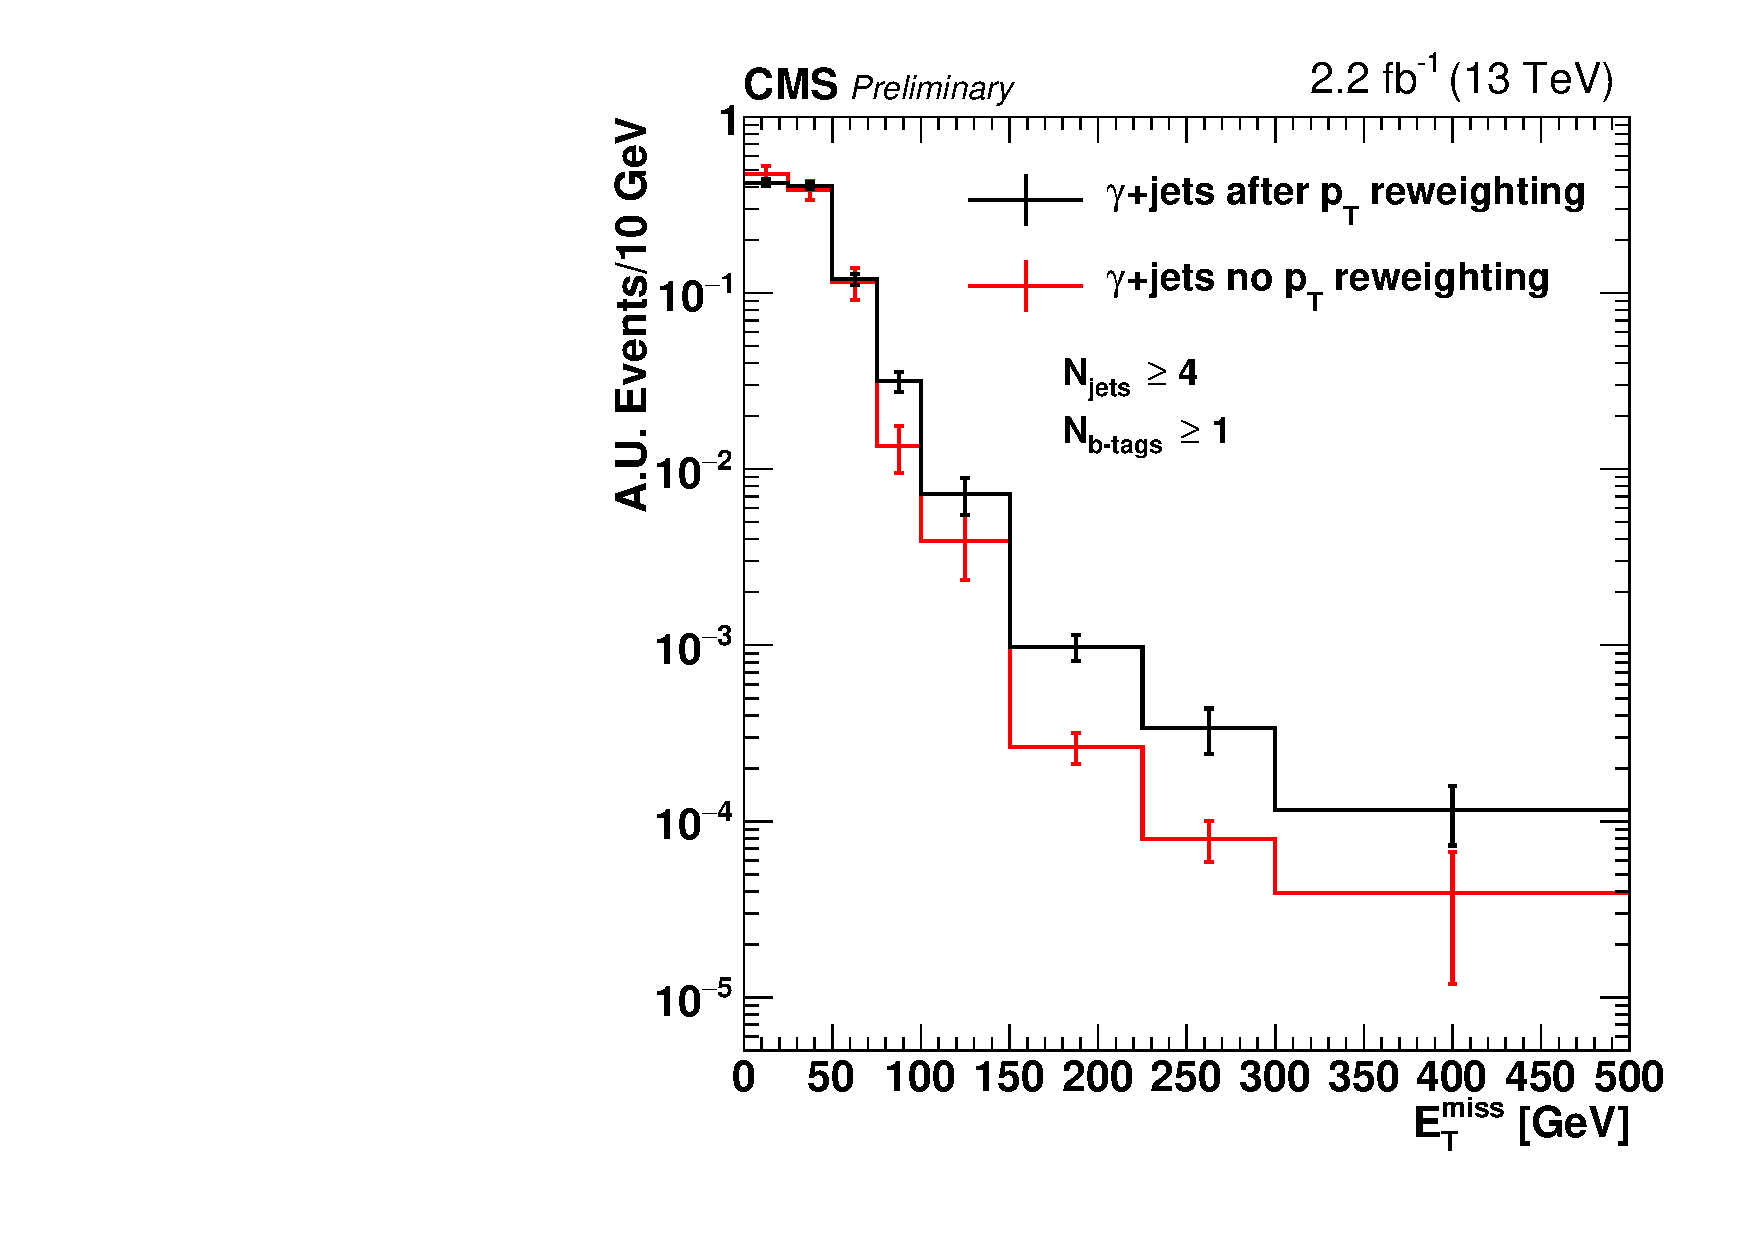
\includegraphics[width=0.8\textwidth]{bkgd/figs/gjets_full2p1_rawMET_withb_SRB_datavsdata_comparereweighted.pdf}
    \end{tabular}
    \caption{
      The \MET\ distributions are shown before reweighting the \gjets\ sample in \pt\ (red) and after reweighting (black)
      for \gjets\ events in signal region B where at least 1 jet is required to be b-tagged.
      The distributions are normalized to unit area.
      \label{fig:metptreweighting}
    }
  \end{center}
\end{figure}

\clearpage

After reweighting in \pt, the resulting \MET distribution is normalized in a region where \zjets\ is the dominant background, namely, \MET\ $<$ 50 \gev.
In order to assess the systematic uncertainties associated with the template method,
a closure test is done using MC simulation where simulated \gjets\ events are used to predict the \MET\ in simulated \zjets\ events.
The closure is assessed separately in each signal region, and uncertainties are assigned based on the results of this closure test.
The uncertainties of this method are described in detail in subsection~\ref{ssec:bkg_zjetssyst}.

\subsection{Systematic Uncertainties in the \texorpdfstring{\MET}{MET}\ Template Prediction}
\label{ssec:bkg_zjetssyst}

The systematic uncertainty in the \MET\ template prediction comes from two sources:
a MC closure study, and the uncertainty associated with normalizing in low \MET.
The largest uncertainty comes from the results of the closure study.
This study is done by generating a \MET\ template using simulated \gjets\ events and using this template to predict the \MET\ for events in simulated \zjets\ events.
This is done using the exact same procedure described in section~\ref{sec:bkg_zjets}.
For the MC closure test, we evaluate the systematic uncertainty separately in various regions including our signal regions.
The results of the closure test are shown for signal region B where at least 1 jet is required to be b-tagged is shown in figure~\ref{fig:SRB_withb_closure} and table~\ref{tab:template_systematics_withb_SRB}.
The uncertainty for each region is chosen to cover the largest descrepancy between the \gjets\ prediction of the \zjets\ MC for each \MET\ region,
or the statistical uncertainty whichever is larger. 
The systematic uncertainty chosen for all regions is listed in table~\ref{tab:template_systematics_overview}.

\begin{figure}[!htb]
  \begin{center}
    \begin{tabular}{cc}
      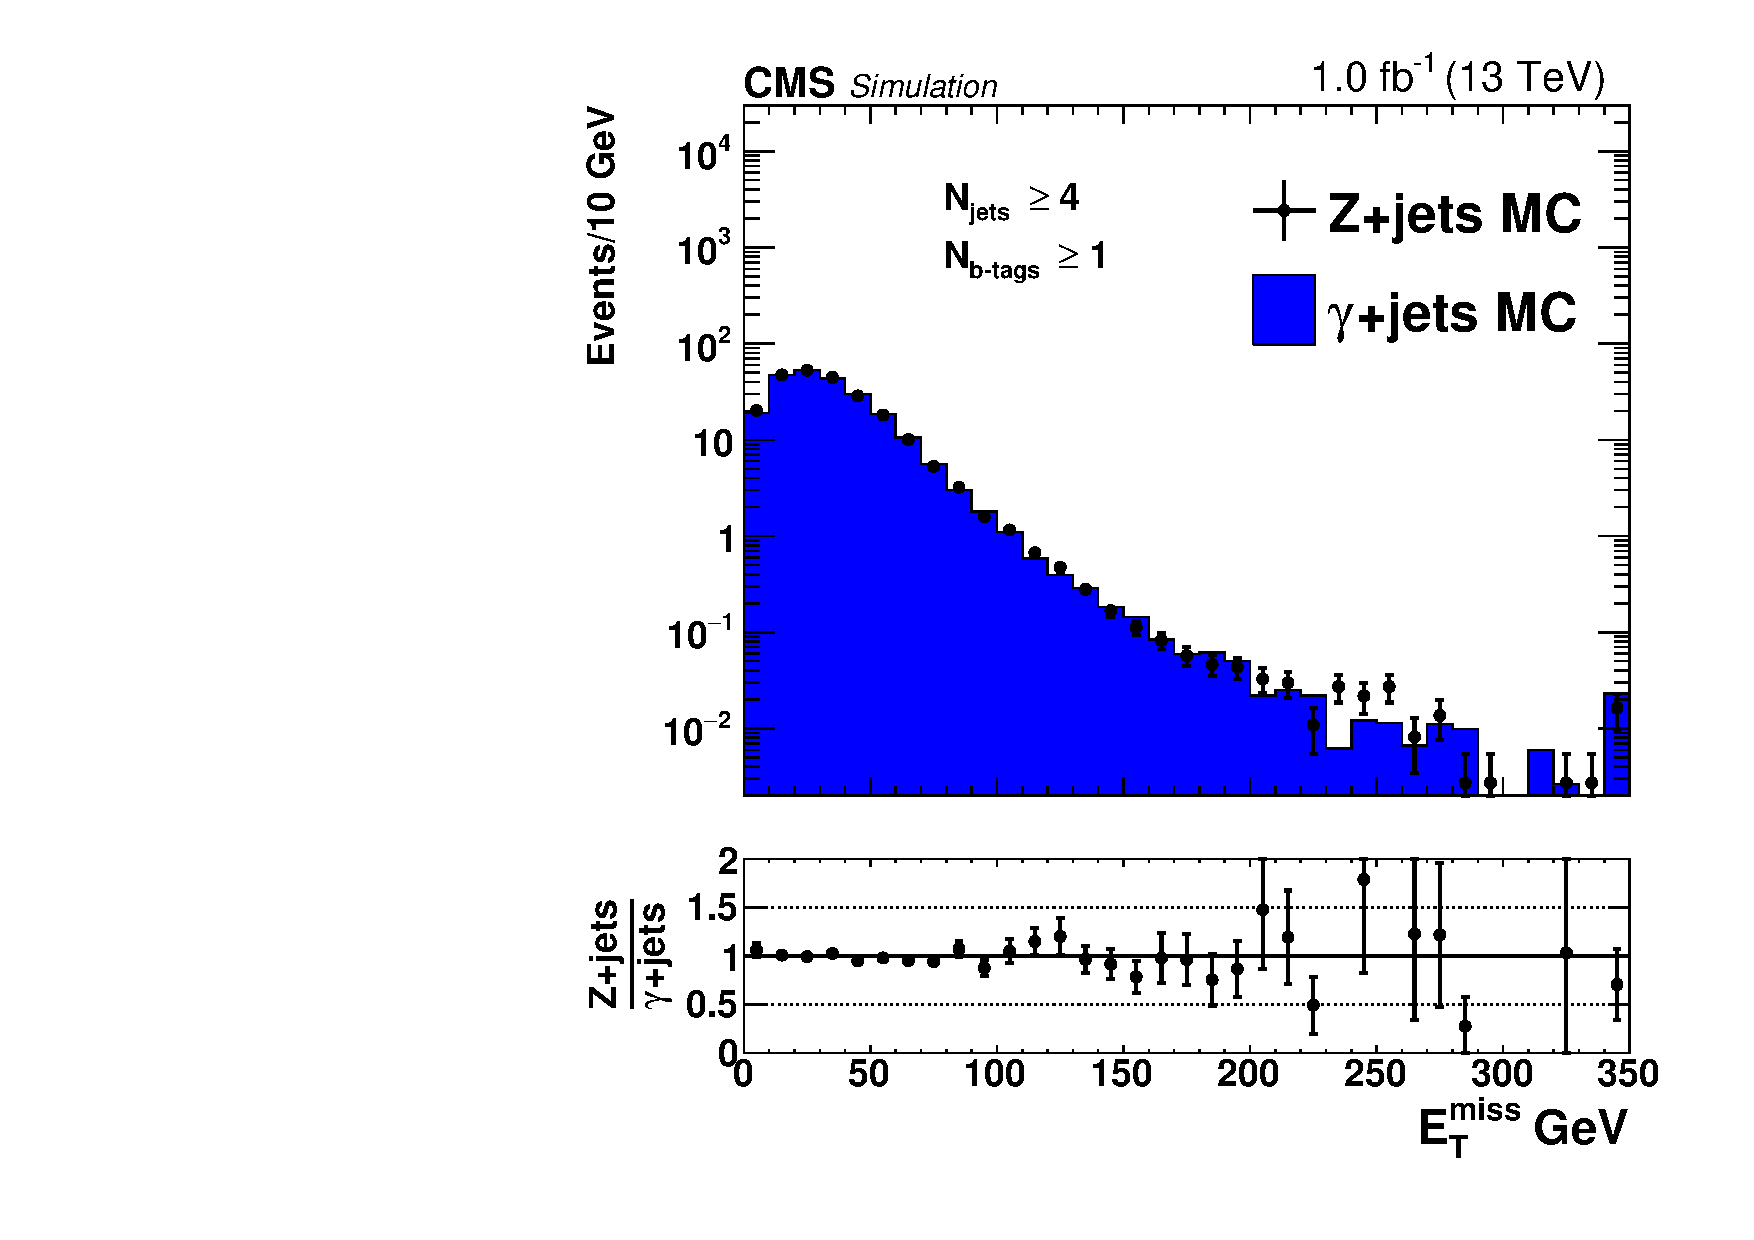
\includegraphics[width=0.8\textwidth]{bkgd/figs/h_met_closure_rawMET_withb_SRB_novtxweight.pdf}
    \end{tabular}
    \caption{
      The closure test for Signal region B where at least 1 jet is required to be b-tagged is shown
      where simulated \gjets\ events are used to predict the \MET\ for simulated \zjets\ events.
      The distributions are normalized to 1 $\mathrm{fb^{-1}}$ of data.
      \label{fig:SRB_withb_closure}
    }
  \end{center}
\end{figure}

\begin{table}[htb]
  \scriptsize
  \begin{center}
    \caption{\label{tab:template_systematics_withb_SRB} 
      Results of the MC closure test shown for signal region B where at least 1 jet is required to be b-tagged.
      The systematic uncertainty for each region is chosen to cover the largest descrepancy between the \gjets\ prediction of the \zjets\ MC for each \MET\ region,
      or the the statistical uncertainty whichever is larger. 
      All uncertainties shown are statistical only. 
    }
    \begin{tabular}{l|c|c|c}
      \hline
      \hline
      $\mathrm{E_{T}^{miss} [GeV]}$ &0 - 50 & 50 - 100 & 100 - 150 \\
      \hline 
      Z+jets&  191.4 $\pm$ 2.9 &  40.5 $\pm$ 0.9 &  2.9 $\pm$ 0.2 \\ 
      $\mathrm{\gamma+jets}$&  190.2 $\pm$ 1.1 &  41.8 $\pm$ 0.5 &  2.7 $\pm$ 0.1 \\ 
      \hline
      ratio&  1.01 $\pm$ 0.02 &  0.97 $\pm$ 0.02 &  1.07 $\pm$ 0.07 \\ 
      \hline
      Uncertainty & 2 \%              & 3 \%              & 10 \%   \\
      \hline
      \hline
      $\mathrm{E_{T}^{miss} [GeV]}$ &150 - 225 & 225 - 300 & $\geq$ 300 \\
      \hline 
      Z+jets&  0.43 $\pm$ 0.03 &  0.11 $\pm$ 0.02 &  0.02 $\pm$ 0.01 \\ 
      $\mathrm{\gamma+jets}$&  0.47 $\pm$ 0.03 &  0.07 $\pm$ 0.01 &  0.03 $\pm$ 0.01 \\ 
      \hline
      ratio&  0.92 $\pm$ 0.10 &  1.50 $\pm$ 0.34 &  0.66 $\pm$ 0.30 \\ 
      \hline
      Uncertainty & 10 \%              & 50 \%              & 50 \%  \\
      \hline
      \hline
    \end{tabular}
  \end{center}
\end{table}

\begin{table}[htb]
  \scriptsize
  \begin{center}
    \caption{
      \label{tab:template_systematics_overview} 
      Systematic uncertainties derived from the MC closure test shown for all the on-Z signal regions. 
      The uncertainties for each region are chosen to cover the largest descrepancy between the \gjets\ prediction of the \zjets\ MC for each \MET\ region,
      or the statistical uncertainty whichever is larger. 
    }
    \begin{tabular}{l|c|c|c|c|c|c}
      \hline
      \hline
      $\mathrm{E_{T}^{miss} [GeV]}$ &0 - 50 & 50 - 100 & 100 - 150  &150 - 225 & 225 - 300 & $\geq$ 300 \\
      \hline 
      SRA, b-veto         & 1 \%              & 4 \%              &  4 \%  &  5 \%              & 15 \%              & 35 \%   \\
      SRA, with b-tags    & 1 \%              & 3 \%              &  5 \%  & 10 \%              & 30 \%              & 40 \%   \\
      \hline
      SRB, b-veto         & 1 \%              & 2 \%              &  4 \%  & 10 \%              & 20 \%              & 25 \%   \\
      SRB, with b-tags    & 2 \%              & 3 \%              & 10 \%  & 10 \%              & 50 \%              & 50 \%   \\
      \hline
      ATLAS Region & 2 \%              & 2 \%              &  10 \%  & 10 \%              & 10 \%              & --   \\
      \hline
      \hline
    \end{tabular}
  \end{center}
\end{table}

\clearpage

The systematic uncertainty associated with the normalization of the template prediction in data in the region with \MET\ from 0-50 \gev\ is assessed in the following way.
The normalization factor is derived by requiring the total background prediction in this region to add up to the yield observed in data.
The uncertainty associated with the ratio of data/prediction is taken as a systematic uncertainty over the entire template prediction.
Table~\ref{tab:template_systematics_reweighting}~shows the uncertainties for each signal region.

\begin{table}[htb]
  \scriptsize
  \begin{center}
    \caption{\label{tab:template_systematics_reweighting} 
      Systematic uncertainties on the normalization procedure are listed in the following table.
    }
    \begin{tabular}{l|c}
      \hline
      \hline
      Signal region & Uncertainty \\
      \hline
      SRA                 &       \\ 
      \hline
      b-veto              &  4\%  \\ 
      $\geq$ 1 b-tag      & 10\%  \\ 
      \hline
      SRB                 &       \\ 
      \hline
      b-veto              &  3\%  \\ 
      $\geq$ 1 b-tag      &  6\%  \\ 
      \hline
      ATLAS Region &  3\%  \\ 
      \hline
      \hline
    \end{tabular}
  \end{center}
\end{table}

\section{Estimating the Flavor-Symmetric Background}
\label{sec:bkg_fs}
The flavor symmetric background method is used to predict standard model backgrounds
where ee and $\mu\mu$ events are equally likely to be produced as e$\mu$ events.
This happens for events where the two leptons each come from a separate W boson.
The largest background that falls into this category is \ttbar,
but other processes that contribute are single top, WW pair production, and events with Z$\rightarrow\tau\tau$ where the taus both decay leptonically.
One important feature of events in this category is that these events all have real \MET\ coming from the associated neutrino production when the W decays leptonically.

This prediction is done using a data control sample of e$\mu$ events.
These events are collected using the e$\mu$ triggers listed in table~\ref{table:triggers},
and a correction is made to this sample to account for the difference in efficiencies of reconstructing and triggering on electrons and muons.
The prediction for the number of same-flavor (SF) events observed ($N_{SF}^{obs.}$)
can be obtained by using the ratio of SF to opposite-flavor (OF) events ($R_{SF/OF}$) multiplied by the number of OF events observed in data($N_{OF}^{obs.}$).
This is done in the following way.

\subsection{\texorpdfstring{$R_{SF/OF}$}{Rsfof}}
The number of observed events in data for each dilepton region is the number of events produced multiplied by the trigger and reconstruction efficiencies,
Therefore the true number of events produced can be obtained from this relation as seen in equation~\ref{eqn:ntrueFSbg}.

\begin{align}
  N_{ee, \mu\mu, e\mu }^{observed} & = N_{ee, \mu\mu, e\mu }^{true} \times (\epsilon_{ee, \mu\mu, e\mu }^{trig.} * \epsilon_{ee, \mu\mu, e\mu }^{reco.})\\
  \label{eqn:ntrueFSbg} N_{ee, \mu\mu, e\mu }^{true} & = \frac{N_{ee, \mu\mu, e\mu }^{observed}}{\epsilon_{ee, \mu\mu, e\mu }^{trig.} * \epsilon_{ee, \mu\mu, e\mu }^{reco.}}
\end{align}

The number of SF events is the sum of ee and $\mu\mu$ events, and the number of OF events is 2$*$ the number of e$\mu$ events.
The factor $2$ in in the number of OF events comes from the combinatorics that arise from not distinguishing $\Pe\mu$ from $\mu\Pe$,
and this also leads to the total number of OF events to be equal to the total number of SF events.

\begin{align}
  \label{eqn:noftrueFSbg} N_{OF}^{true} & = N_{SF}^{true}\\  
  N_{SF} & \equiv N_{ee} + N_{\mu\mu}\\ 
  N_{OF} & \equiv N_{e\mu}+N_{\mu e} = 2 * N_{e\mu}
\end{align}

Combining this information, \rsfof\ can be written in terms of purely the trigger and reconstruction efficiencies as seen in equation~\ref{eqn:RSFOF}.

\begin{align}
  \label{eqn:RSFOF} R_{SF/OF}     & = \frac{N_{SF}^{obs.}}{N_{OF}^{obs.}}
  = \frac{\epsilon_{\Pe\Pe}^\mathrm{reco.}\epsilon_{\Pe\Pe}^\mathrm{trig.} + \epsilon_{\mu\mu}^\mathrm{reco.}\epsilon_{\mu\mu}^\mathrm{trig.}}{2\epsilon_{e\mu}^\mathrm{reco.}\epsilon_{e\mu}^\mathrm{trig.}}
\end{align}

These ratios are be measured in appropriate SF and OF control regions.

\clearpage

The value for \rsfof\ can also be calculated in a separate way which underlines
the advantage of using the combined SF sample compared to the separate ee and $\mu\mu$ samples
and is done by measuring two quantities, \rmue\ and \rt.
\rmue is the ratio of the number of $\mu$s reconstructed to the number of reconstructed electrons, shown in equation~\ref{eqn:rmue}.
\rt\ is the square root of the ratio of the number SF events to OF events, shown in equation~\ref{eqn:rt}.
While $R_{\ell\ell/OF}$ is directly affected by the differences in reconstruction and trigger efficiencies by the factors \rmue 
or $r_{\mu/e}^{-1}$, these differences partially cancel out in \rsfof.

\begin{align}
  \label{eqn:rmue} r_{\mu/e} & \equiv \sqrt{\frac{N_{\mu\mu}}{N_{\Pe\Pe}}} 
  = \sqrt{\frac{\epsilon_{\mu\mu}^\mathrm{reco.}\epsilon_{\mu\mu}^\mathrm{trig.}}{\epsilon_{\Pe\Pe}^\mathrm{reco.}\epsilon_{\Pe\Pe}^\mathrm{trig.}}} \\
  \label{eqn:rt} R_T   & \equiv 2 \frac{\sqrt{N_{\Pe\Pe}N_{\mu\mu}}}{N_{OF}} 
  = \frac{\sqrt{\epsilon_{\Pe\Pe}^\mathrm{reco.}\epsilon_{\Pe\Pe}^\mathrm{trig.}\epsilon_{\mu\mu}^\mathrm{reco.}\epsilon_{\mu\mu}^\mathrm{trig.}}}{\epsilon_{OF}^\mathrm{reco.}\epsilon_{OF}^\mathrm{trig.}},
\end{align}

\rsfof\ is then derived using these equations according to equation~\ref{masterformulaExpAlt}.

\begin{align}
  \label{masterformulaExpAlt}
  R_{\Pe\Pe/OF} & = \frac{N_{\Pe\Pe}}{N_{OF}} 
  = \frac{1}{2} \sqrt{\frac{N_{\Pe\Pe}}{N_{\mu\mu}}} \times 2 \frac{\sqrt{N_{\Pe\Pe}N_{\mu\mu}}}{N_{OF}} = \frac{1}{2} r_{\mu/e}^{-1} \times R_T \notag \\
  R_{\mu\mu/OF} & = \frac{N_{\mu\mu}}{N_{OF}} 
  = \frac{1}{2} \sqrt{\frac{N_{\mu\mu}}{N_{\Pe\Pe}}} \times 2 \frac{\sqrt{N_{\Pe\Pe}N_{\mu\mu}}}{N_{OF}} = \frac{1}{2} r_{\mu/e} \times R_T \notag\\
  R_{SF/OF} & = R_{\Pe\Pe/OF}+R_{\mu\mu/OF} = \frac{1}{2} (r_{\mu/e} + r_{\mu/e}^{-1})\times R_T. 
\end{align}

The final value of \rsfof\ is calculated in two ways.
The first is a direct measurement of the ratio in data in a control region enriched in \ttbar\ described in subsection~\ref{ssec:rsfofDirect},
while the second consists of the separated estimation of the \rmue and $R_T$ factors described in subsection~\ref{ssec:rsfoffactorization}.

\subsection{Direct measurement of \texorpdfstring{\rsfof}{Rsfof}}
\label{ssec:rsfofDirect}
\rsfof is measured directly in a control region enriched in \ttbar.
This region is orthogonal to the signal regions and defined below.

\begin{itemize}
\item the same lepton selection
\item exactly two jets
\item \met between 100 and 150 GeV
\end{itemize}

The results of this direct measurement of \rsfof are displayed in figure~\ref{fig:rsfof} and table~\ref{tab:rSFOF}
where values of MC simulation and data are compared for the aforementioned control region.
The values from \ttbar MC are shown for comparison in the signal region and in low-mass, and high-mass regions.
Additionally, the leptons are classified into two regions, ``central'' and ``forward''.
For events to be considered central, both leptons must have $|\eta| < 1.4$,
and for events to be considered forward, at least one lepton must have $|\eta| > 1.6$.
This is done since the leptons measured in the barrel region have better resolution,
so it can be checked that the resolution does not degrade when leptons are measured in the forward region.
The two values are combined using a weighted average for the final result.
The values measured in data for \rsfof\ shown in figure~\ref{fig:rsfof} agree with the measurement made in MC within the uncertainties,
and both measured values are close to 1.

\begin{figure}[htb]
  \begin{center}
    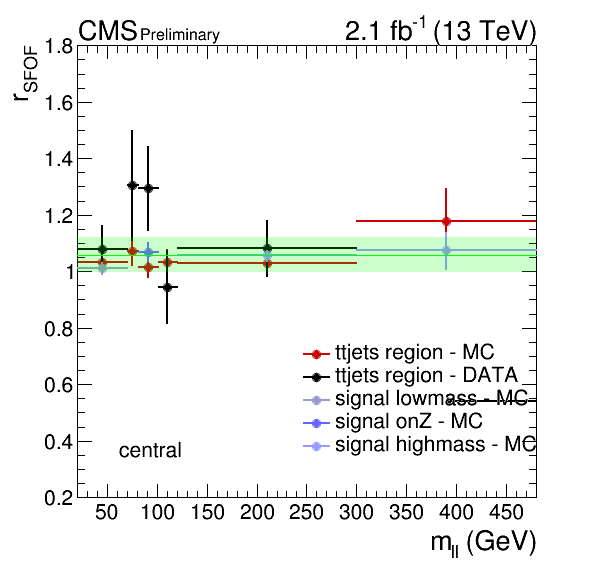
\includegraphics[scale=0.35]{bkgd/figs/plot_rsfof_mll_central.png}
    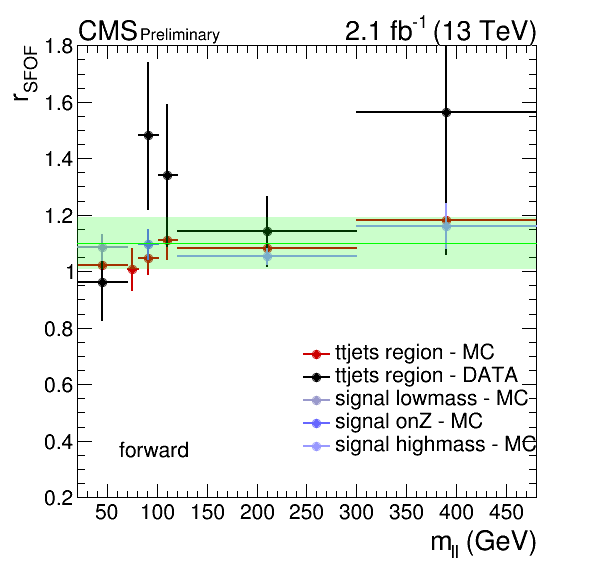
\includegraphics[scale=0.35]{bkgd/figs/plot_rsfof_mll_forward.png}
    \caption{
      Direct measurement of \rsfof in the control region for data (black) and \ttbar MC (red).
      Values in the signal region are shown in blue for \ttbar MC. Central rapidity is shown on the left and forward rapidity on the right.
      The green band represents the overall uncertainty on the measured value of \rsfof.
    }
    \label{fig:rsfof}
  \end{center}
\end{figure}

The numerical values of the correction factors are obtained in the low-mass and high-mass regions combined,
excluding the on-Z region because of the contamination with Drell--Yan backgrounds.
They are shown in Tab.~\ref{tab:rSFOF}.
The results from data and MC agree well within their uncertainties and are close to unity.
To study the extrapolation of the measured value into the signal region,
the ratio of \rsfof in the control and signal region on simulation is studied.
It is found to be compatible with unity within the statistical uncertainty of the simulation.
This statistical uncertainty is therefore assigned as the systematic uncertainty of this method.
\begin{table}[hbt]
  \begin{center}
    \caption{
      Observed event yields in the control region and the resulting values of \Rsfof, \Reeof, and \Rmmof.
      The results are shown separately for the central and forward lepton selection and the same quantities derived on simulation are shown for comaprison.
    }
    \label{tab:rSFOF}
    \begin{tabular}{l|c|c|c|c}     
      & $N_{SF}$ & $N_{OF}$ & \Rsfof $ \pm \sigma_{stat}$ & Transfer factor $\pm \sigma_{stat}$  \\    
      \hline
      &  \multicolumn{4}{c}{Central} \\
      \hline
      Data & 668 & 631 & 1.059$\pm$0.059 & -- \\
      MC & 790.9 & 753.2 & 1.050$\pm$0.013 & 0.980$\pm$0.016\\ 
      \hline 
      & \multicolumn{4}{c}{Forward} \\
      \hline
      Data & 339 & 306 & 1.108$\pm$0.087 & -- \\
      MC & 389.3 & 360.9 & 1.079$\pm$0.021 & 1.018$\pm$0.026\\
      \hline\hline
      & $N_{ee}$ & $N_{OF}$ & \Reeof$ \pm \sigma_{stat}$ & Transfer factor $\pm \sigma_{stat}$  \\    
      \hline
      &  \multicolumn{4}{c}{Central} \\
      \hline
      Data & 269 & 631 & 0.426$\pm$0.031 & -- \\
      MC & 339.0 & 753.2 & 0.450$\pm$0.007 & 0.988$\pm$0.020\\
      \hline 
      & \multicolumn{4}{c}{Forward} \\
      \hline
      Data & 141 & 306 & 0.461$\pm$0.047 & -- \\
      MC & 157.4 & 360.9 & 0.436$\pm$0.011 & 1.023$\pm$0.036\\
      \hline\hline
      & $N_{\mu\mu}$ & $N_{OF}$ & \Rmmof $ \pm \sigma_{stat}$ & Transfer factor $\pm \sigma_{stat}$  \\    
      \hline
      & \multicolumn{4}{c}{Central} \\
      \hline
      Data & 399 & 631 & 0.632$\pm$0.040 & -- \\
      MC & 451.9 & 753.2 & 0.600$\pm$0.009 & 0.974$\pm$0.019\\
      \hline 
      & \multicolumn{4}{c}{Forward} \\
      \hline
      Data & 198 & 306 & 0.647$\pm$0.059 & -- \\
      MC & 232.0 & 360.9 & 0.643$\pm$0.015 & 1.013$\pm$0.030\\
    \end{tabular}  
  \end{center}
\end{table}

\subsection{Measureing \texorpdfstring{\rsfof}{Rsfof} using the Factorization Method}
\label{ssec:rsfoffactorization}
\rmue and \rt are measured in data in order to calculate \rsfof according to Eq.~\ref{masterformulaExpAlt}.

The measurement of \rmue is performed in a Drell--Yan enriched control region
which takes advantage the large number of ee and $\mu\mu$ pairs from \Z boson decays.
This region is defined as having \MET $<$ 50 GeV, and at least two jets.
The invariant dilepton mass is then required to be near the \Z boson mass,
60\GeV $<$ \mll $<$ 120\GeV.

The observed event yields in the two channels are shown in table~\ref{tab:rMuE},
together with the resulting value of \rmue.
The results on MC are shown for comparison.
It can be seen that the efficiency for muons is higher than for electrons by 10\%
for central leptons and by 20\% in the forward region.
Consistent results are observed in the simulation.

\begin{table}[hbtp]
  \begin{center}
    \caption{
      \label{tab:rMuE}
      Result of the calculation of \rmue.
      The observed event yields are shown in the Drell--Yan control region for the central and forward lepton selection in the ee and $\mu\mu$ channels
      and the resulting values of \rmue.
      The same quantaties derived from simulation are shown for comparison.
    }
    \begin{tabular}{l| ccc }
      & $N_{\mu\mu}$ &  $N_{ee}$ & \rmue $\pm \sigma_{\text{stat.}} \pm \sigma_{\text{syst.}}$ \\ 
      \hline
      & \multicolumn{3}{c}{Central}  \\ 
      \hline
      Data     &  23533                   & 18238              &  1.14$\pm$0.01$\pm$0.11    \\
      MC       &  30400                   & 23711              &  1.13$\pm$0.00$\pm$0.11    \\
      \hline
      & \multicolumn{3}{c}{Forward}  \\ 
      \hline
      Data     &  14937                   &  9807              &  1.23$\pm$0.01$\pm$0.25    \\
      MC       &  19449                   & 12287              &  1.26$\pm$0.01$\pm$0.25    \\
    \end{tabular}
  \end{center}
\end{table}

The function in equation~\ref{masterformulaExpAlt} where \rmue\ is used is studied as a function of kinematic variables that are relevant to the search.
Specifically, the function 0.5($r_{\mu e}+1/r_{\mu e}$) is plotted as a function of \nj, \nvtx, lepton \pt, \mll, \MET, and $N_{b-tags}$.
The result of these studies is shown for central and forward leptons in figures~\ref{fig:RDependencyCentral} and~\ref{fig:RDependencyForward}.
The dashed line illustrates the central value observed in data.
No significant dependency on lepton \pt is observed, 
and the value of \rmue is especially stable with respect to \nj and \MET.
No dependency is observed on the number of reconstructed vertices showing that \rmue is insensitive to pileup.   
a systematic uncertainty of 10\%(20\%) is assigned in the central (forward) lepton selection based on these results.

\begin{figure}[htbp]
  \begin{center}
    \begin{tabular}{ccc}
      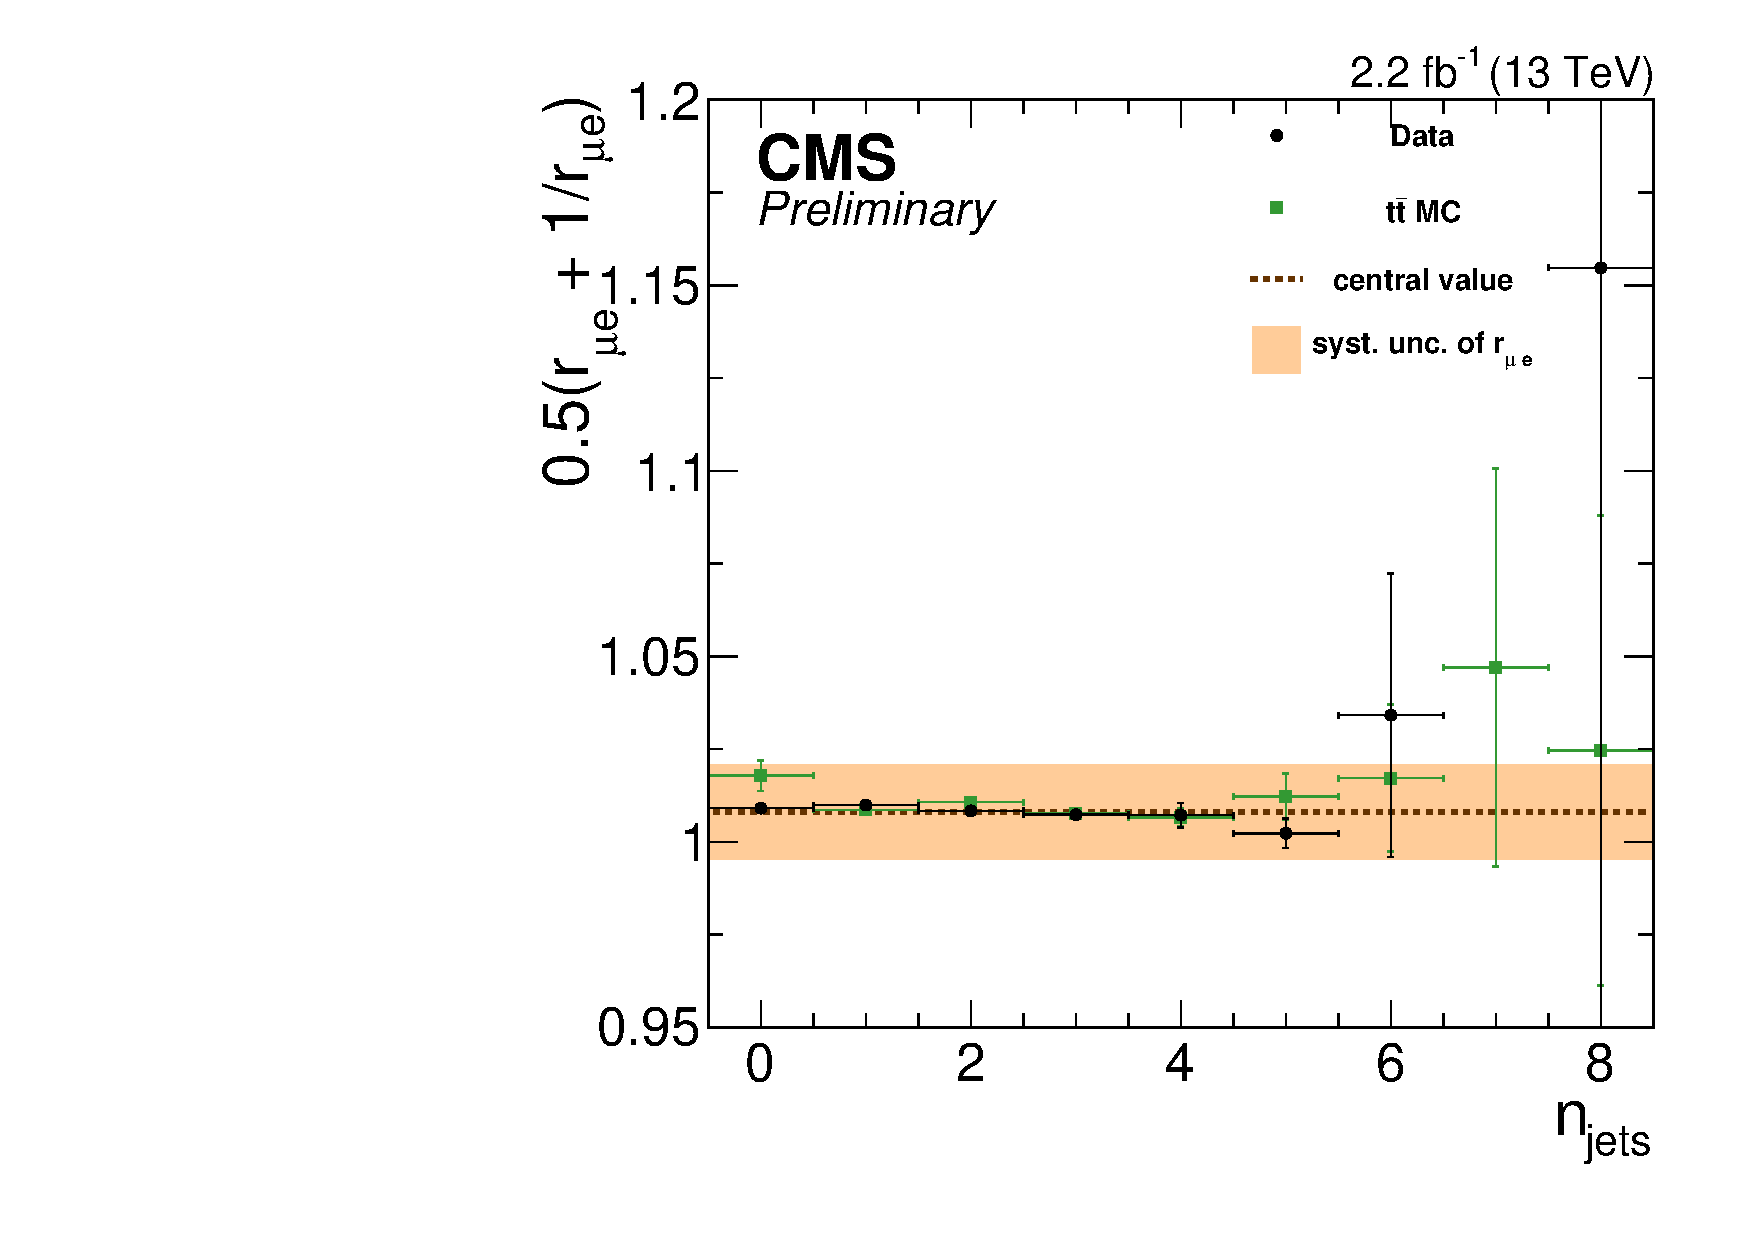
\includegraphics[width=0.30\textwidth]{bkgd/figs/rSFOFFromRMuE_ZPeakControlCentral_Run2015_25ns_NJets_None.pdf} & 
      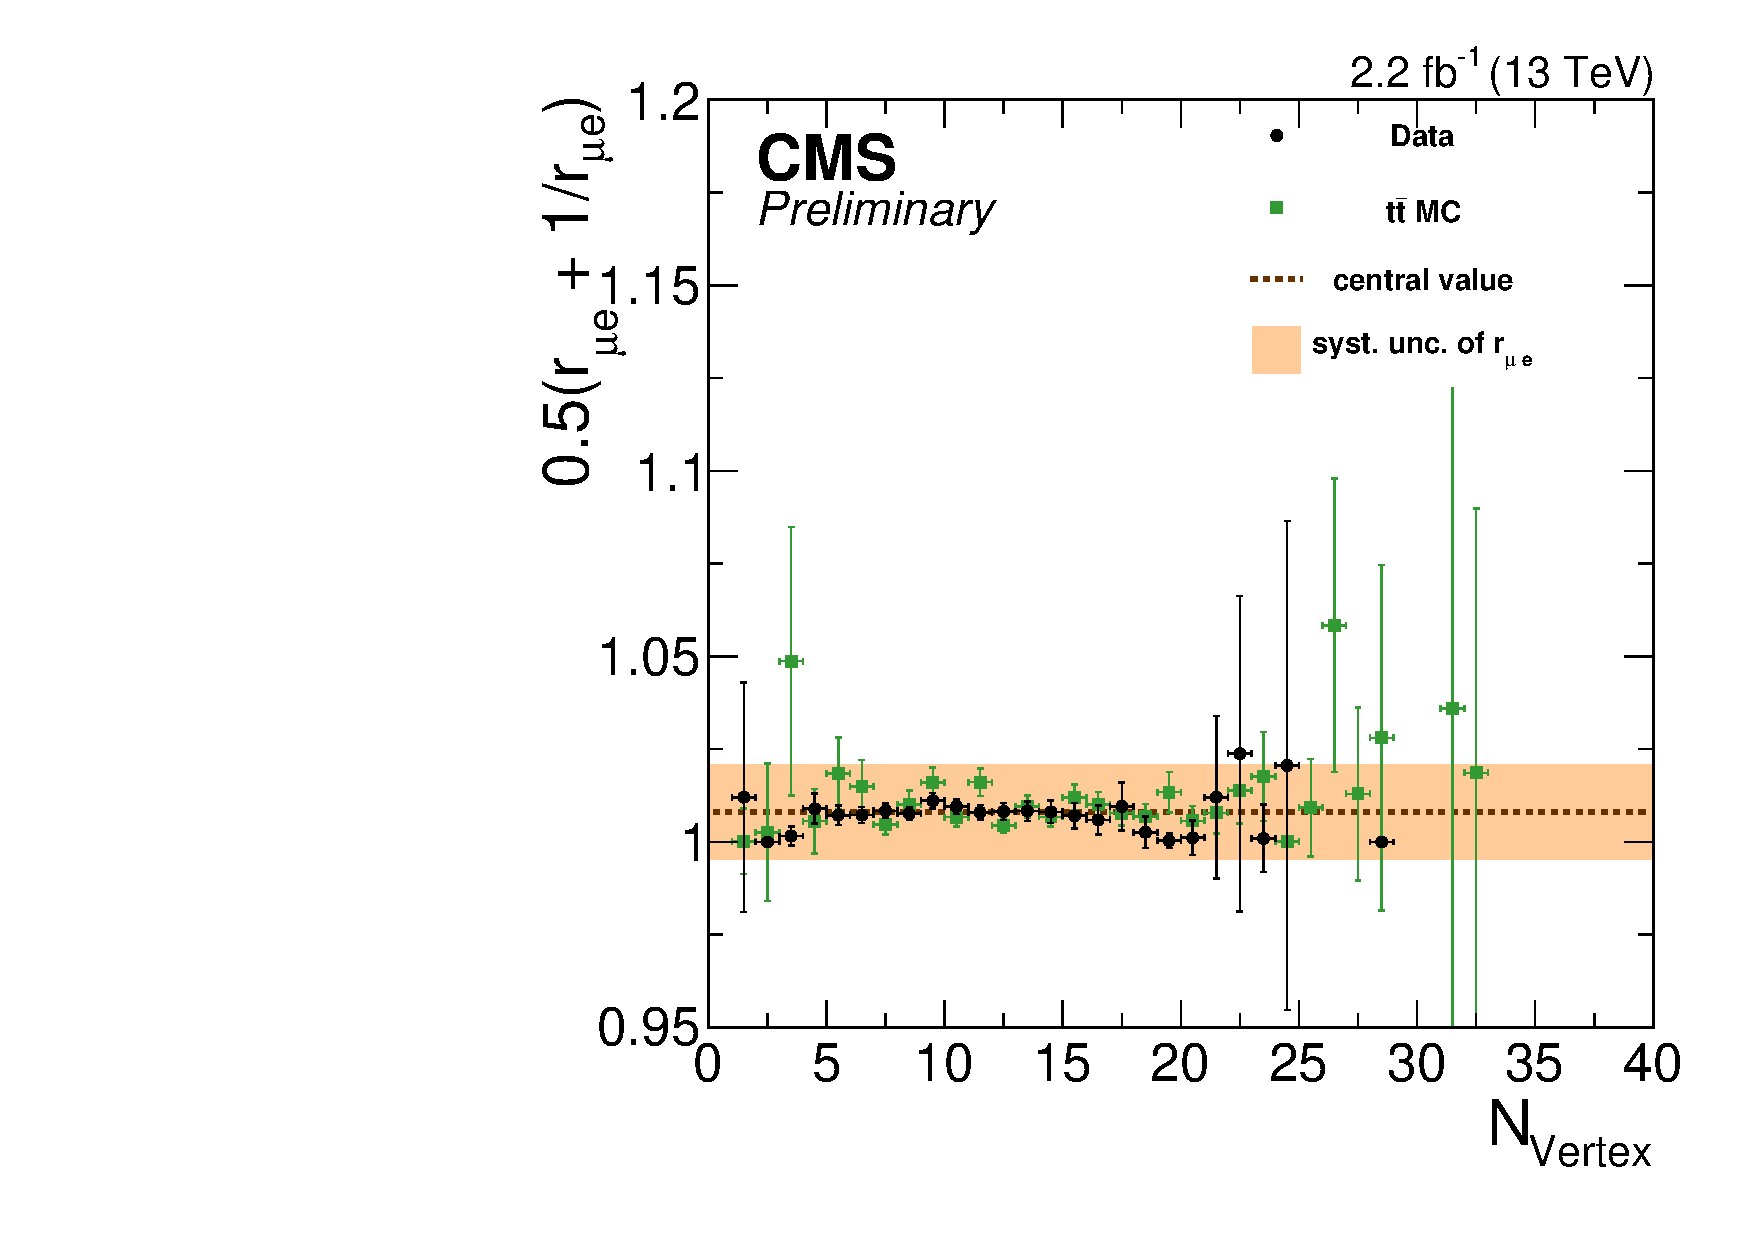
\includegraphics[width=0.30\textwidth]{bkgd/figs/rSFOFFromRMuE_ZPeakControlCentral_Run2015_25ns_nVtx_None.pdf}  &
      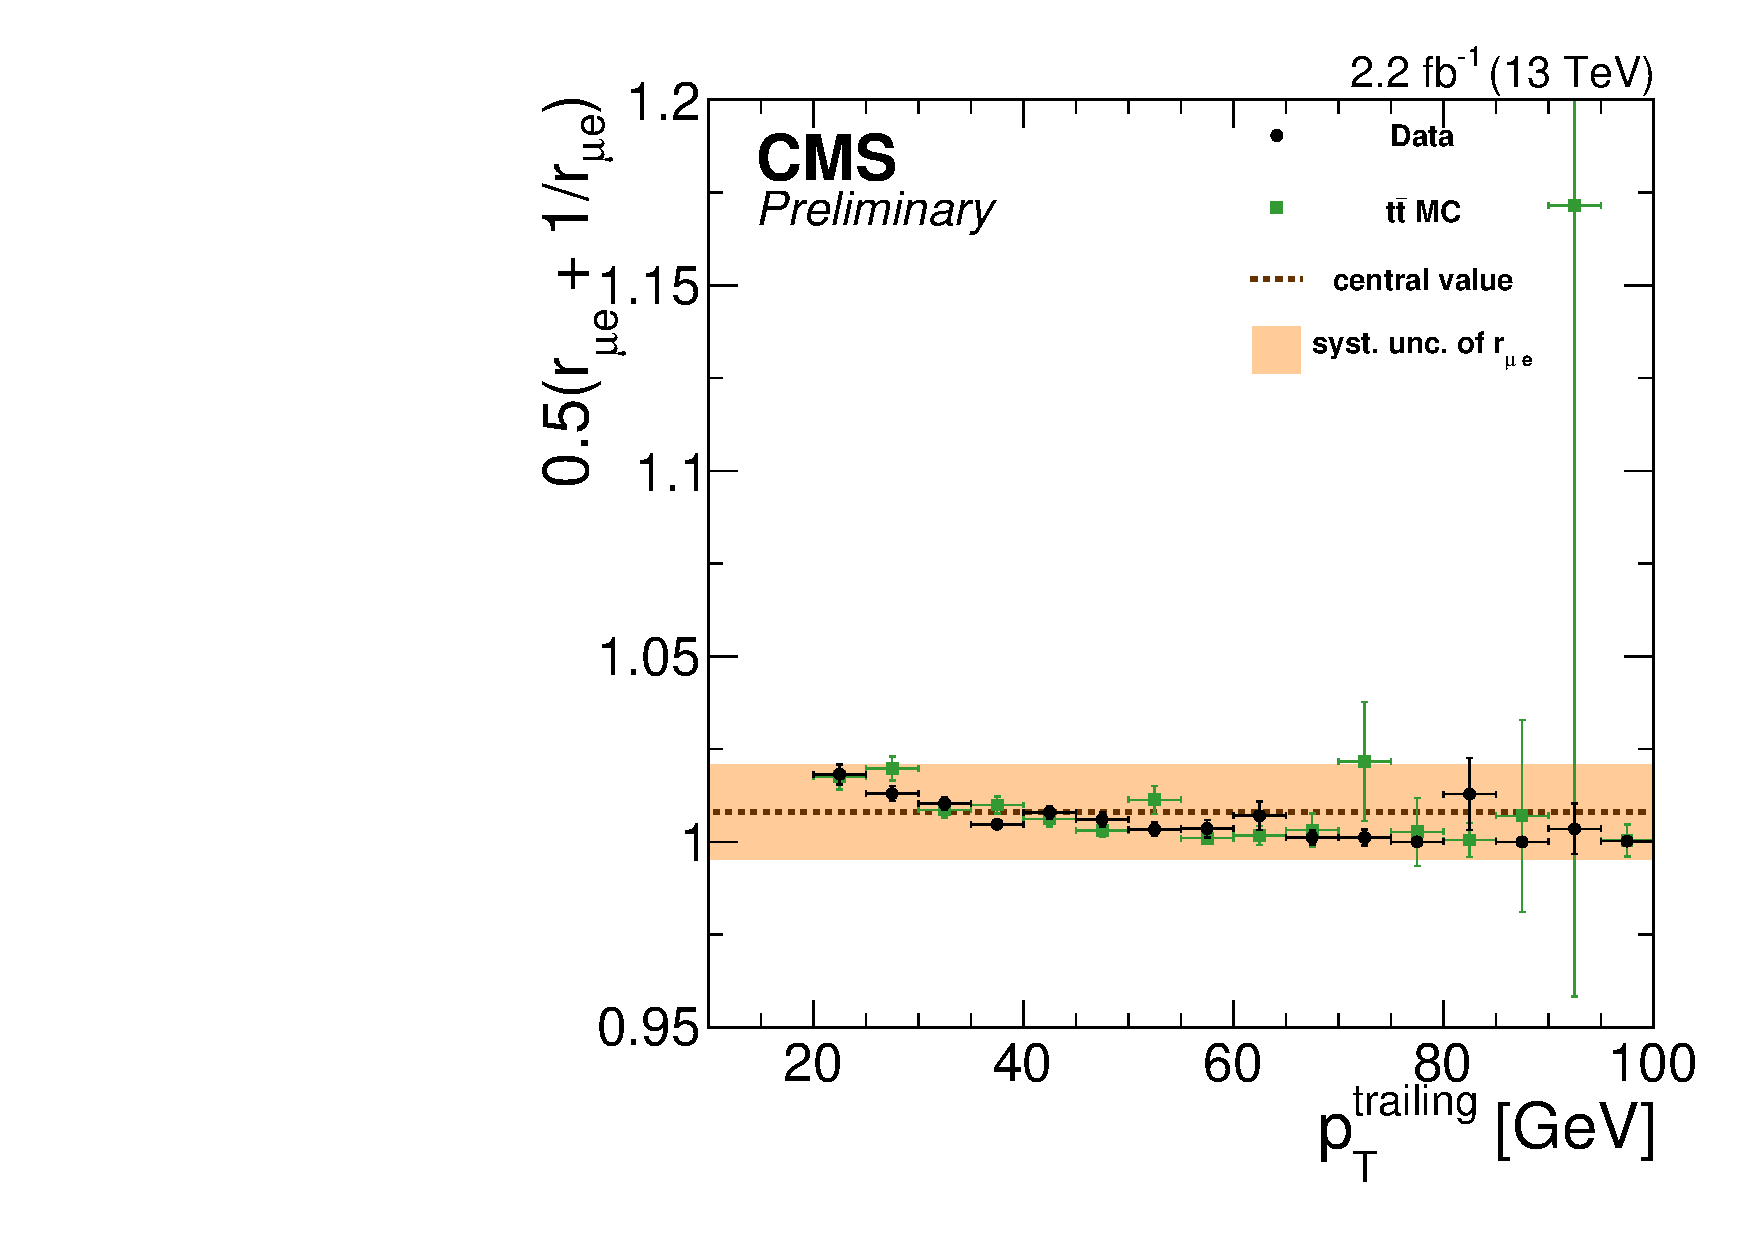
\includegraphics[width=0.30\textwidth]{bkgd/figs/rSFOFFromRMuE_ZPeakControlCentral_Run2015_25ns_TrailingPt_None.pdf} \\
      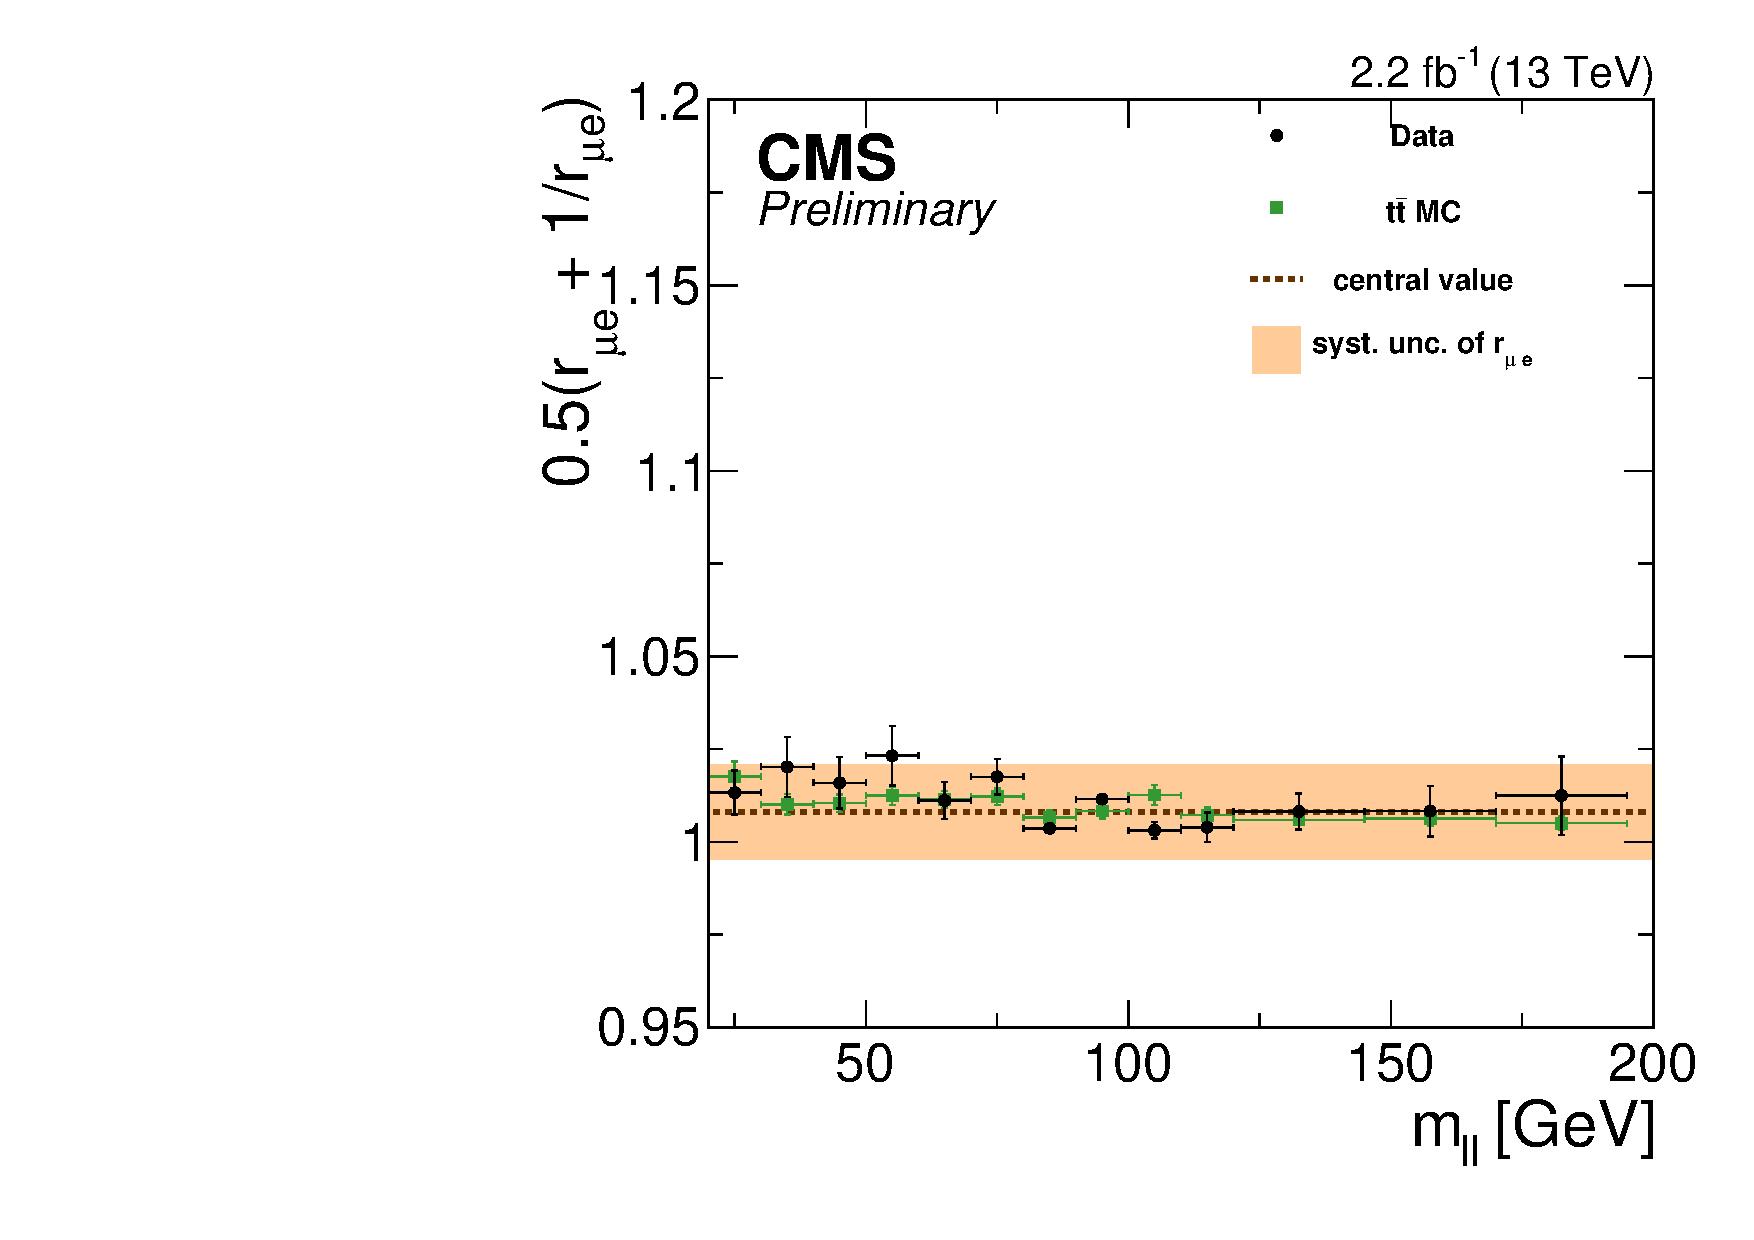
\includegraphics[width=0.30\textwidth]{bkgd/figs/rSFOFFromRMuE_ZPeakControlCentral_Run2015_25ns_Mll_None.pdf} &
      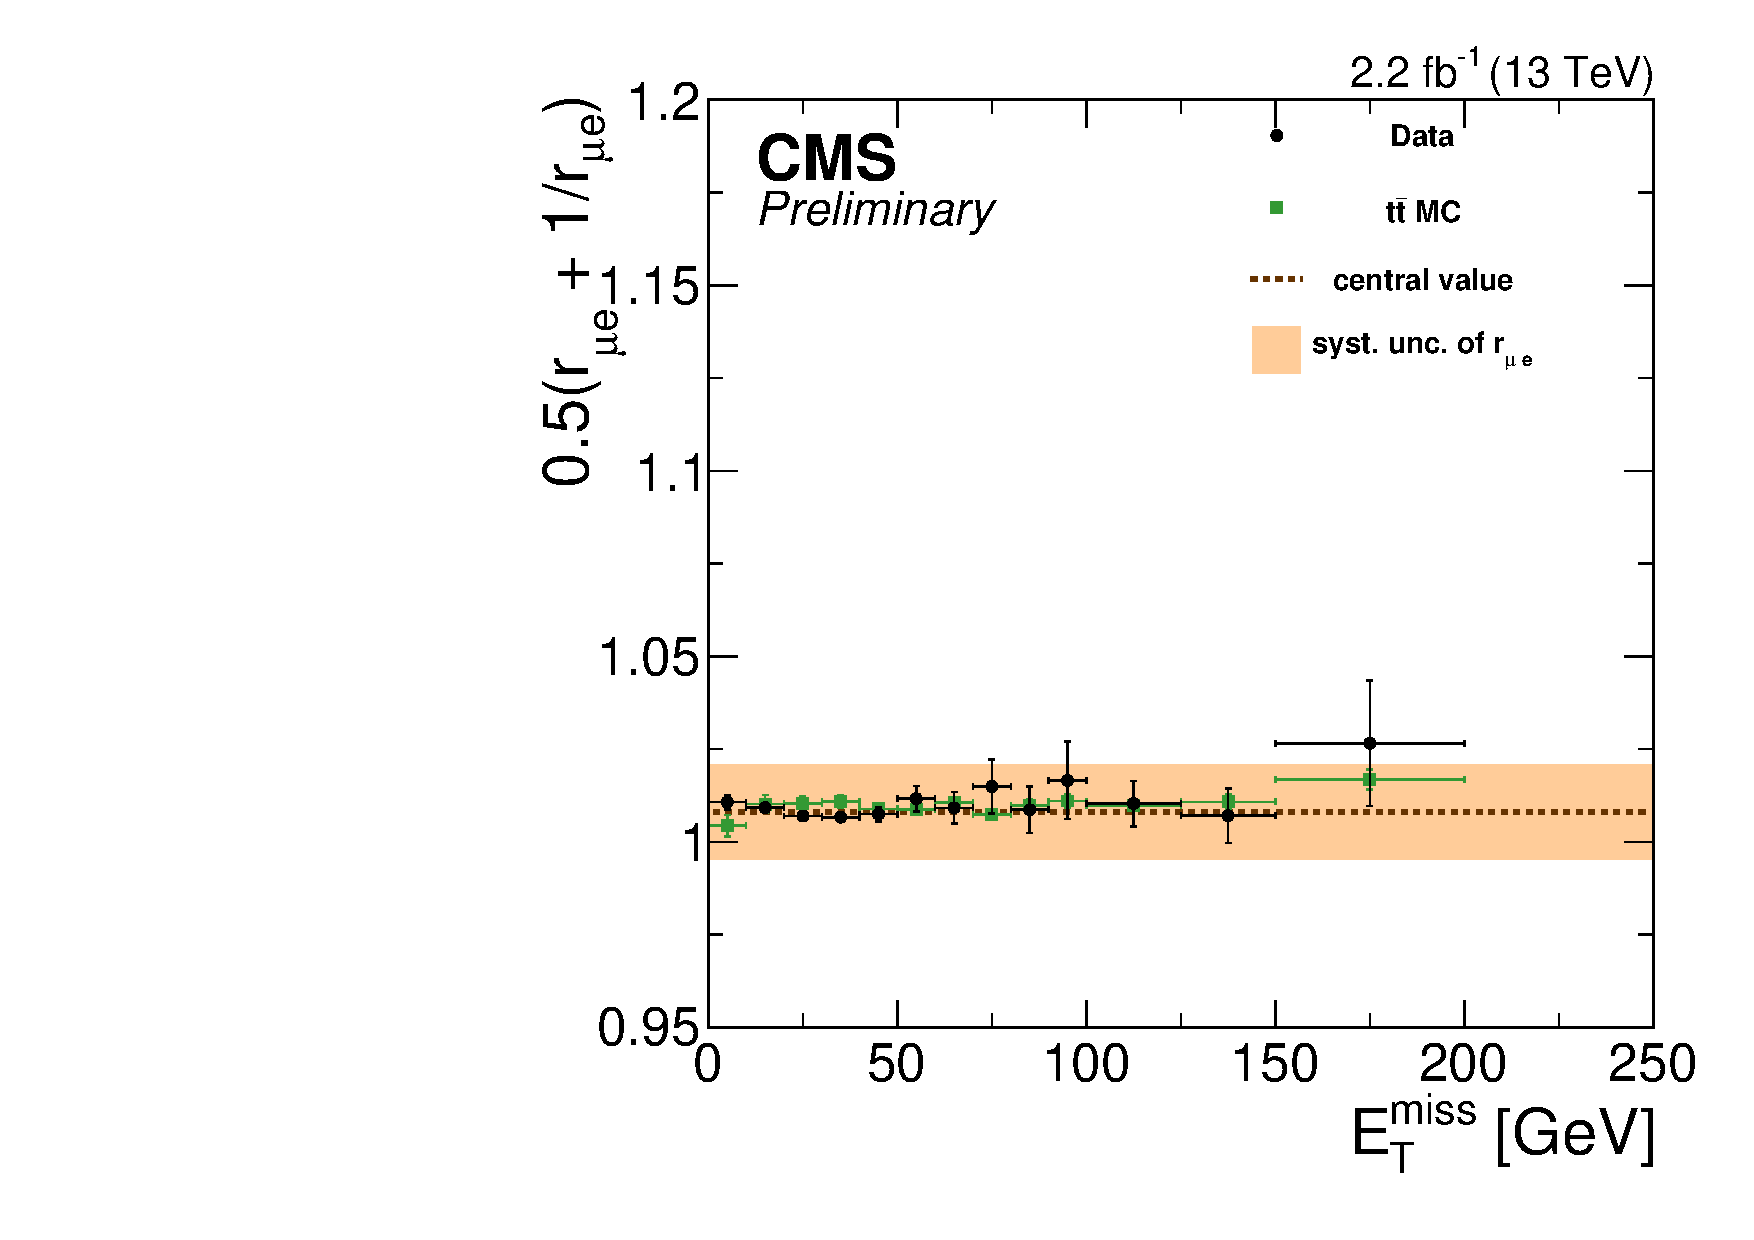
\includegraphics[width=0.30\textwidth]{bkgd/figs/rSFOFFromRMuE_ZPeakControlCentral_Run2015_25ns_MET_None.pdf} &
      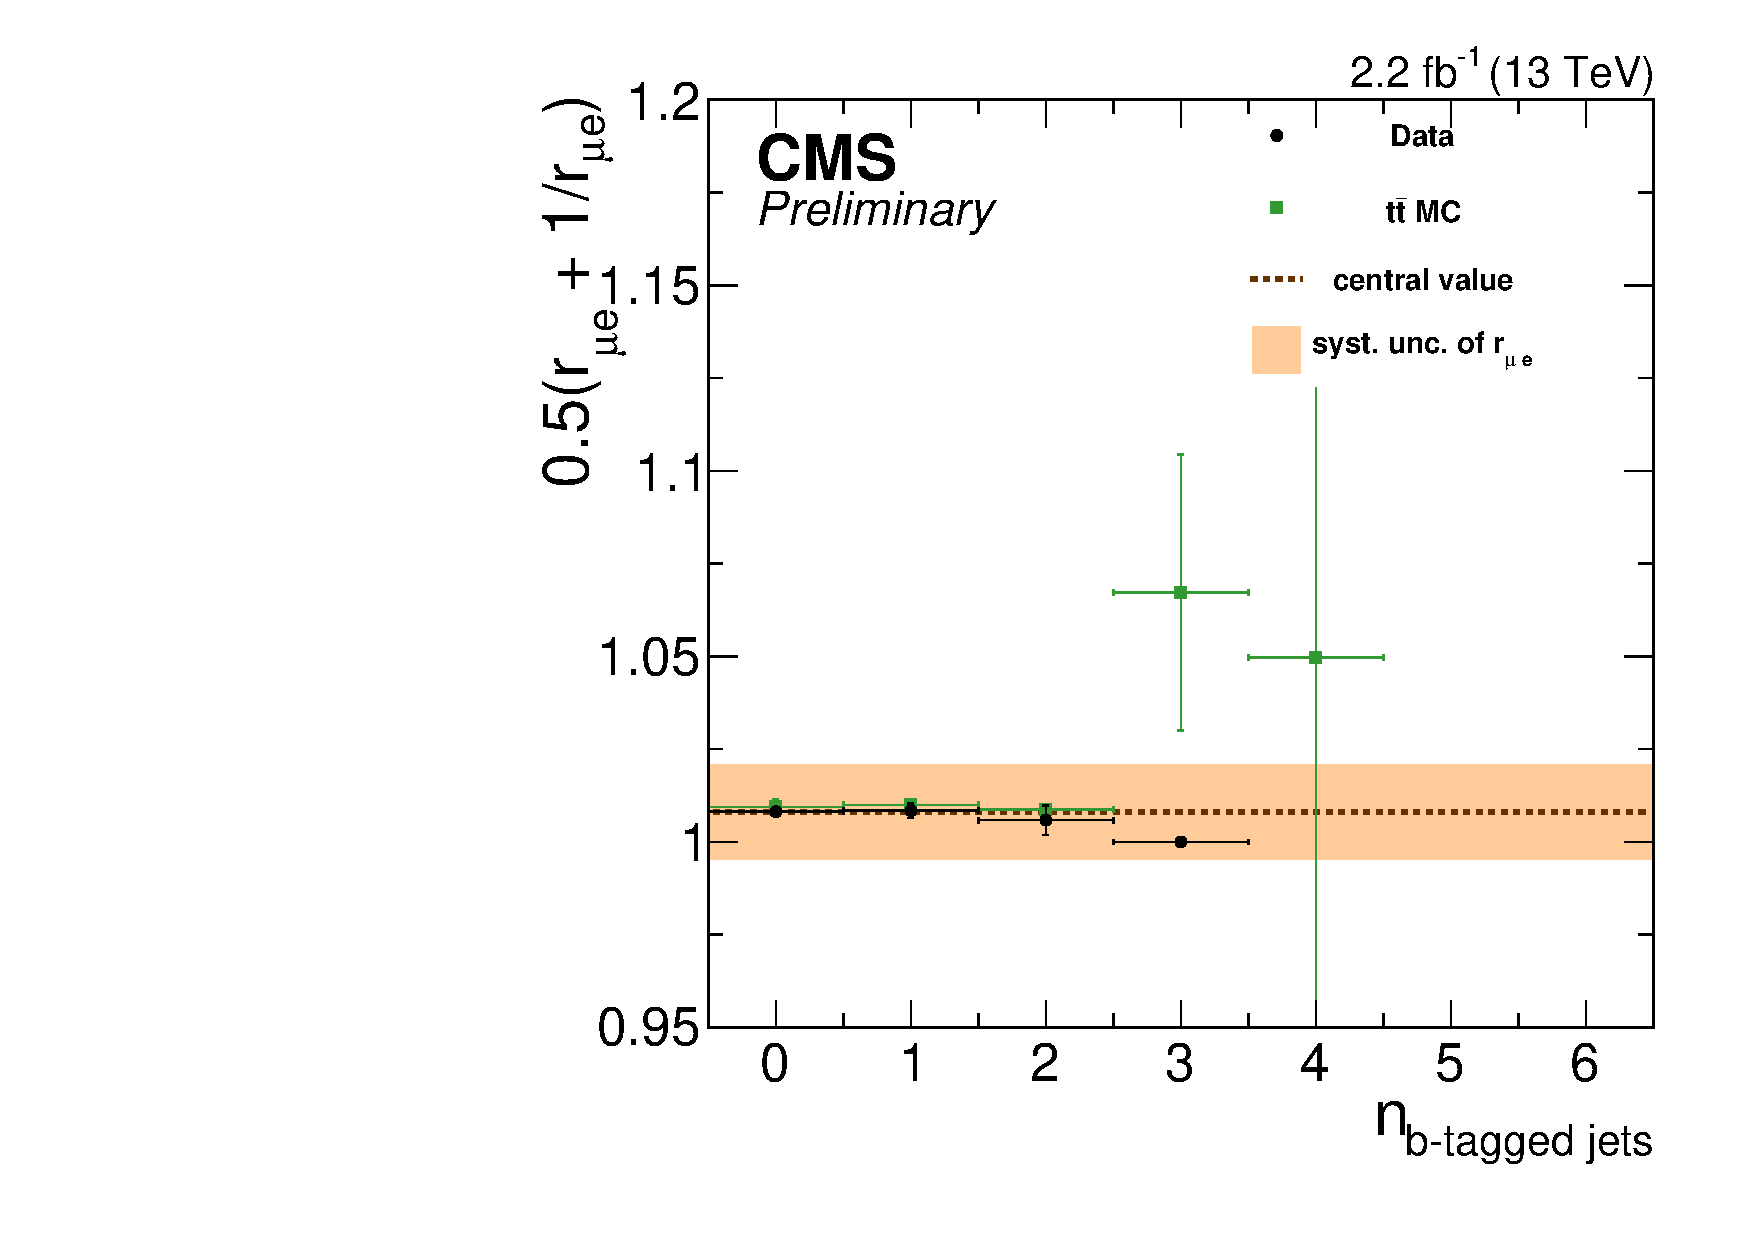
\includegraphics[width=0.30\textwidth]{bkgd/figs/rSFOFFromRMuE_ZPeakControlCentral_Run2015_25ns_NBJets_None.pdf} \\
    \end{tabular}
  \end{center}
  \caption{
    \label{fig:RDependencyCentral}
    0.5($r_{\mu e}+1/r_{\mu e}$) dependency for central leptons shown as a function of \nj, \nvtx, lepton \pt, \mll, \MET, and $N_{b-tags}$.
    The uncertainty due to the assigned 10\% systematic uncertainty on \rmue~is indicated by the orange band.
  }
\end{figure}

\begin{figure}[htbp]
  \begin{center}
    \begin{tabular}{ccc}
      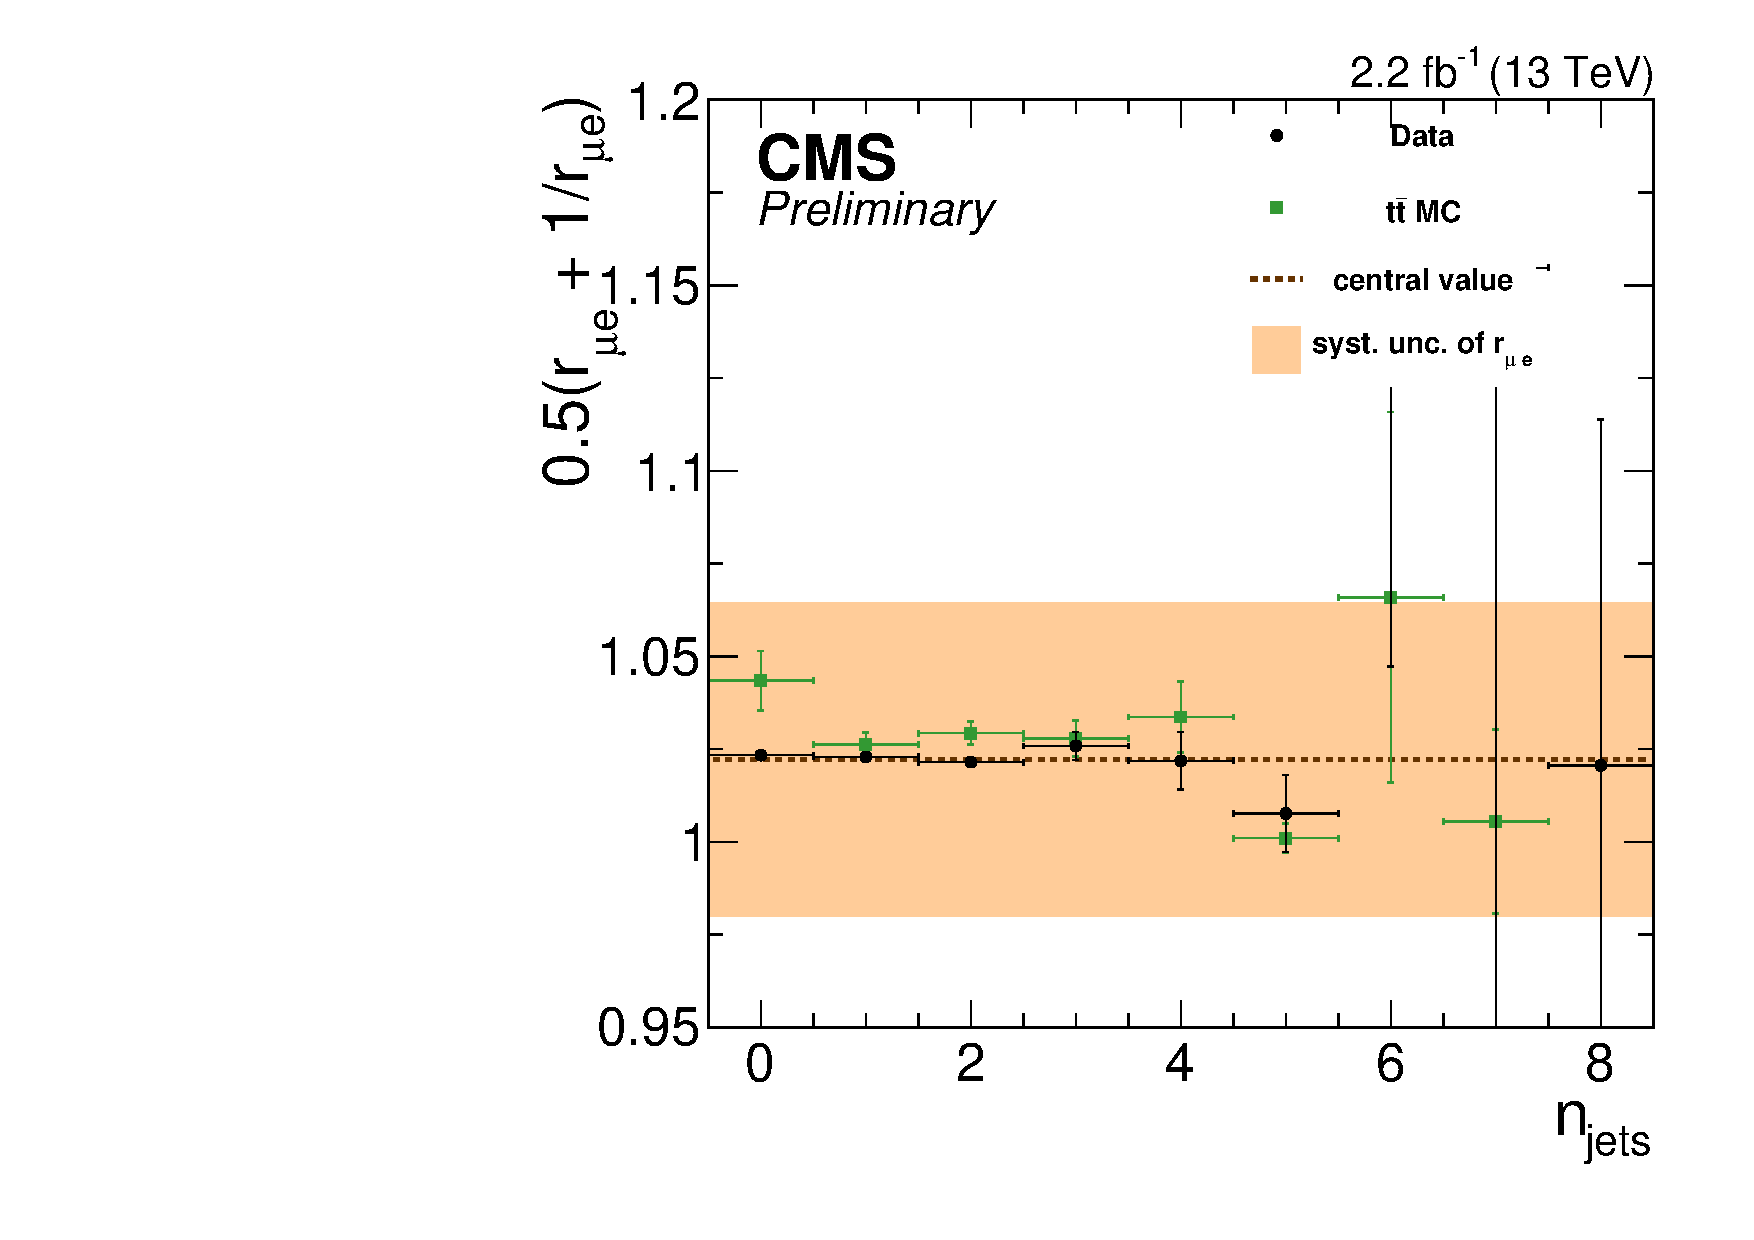
\includegraphics[width=0.30\textwidth]{bkgd/figs/rSFOFFromRMuE_ZPeakControlForward_Run2015_25ns_NJets_None.pdf} &
      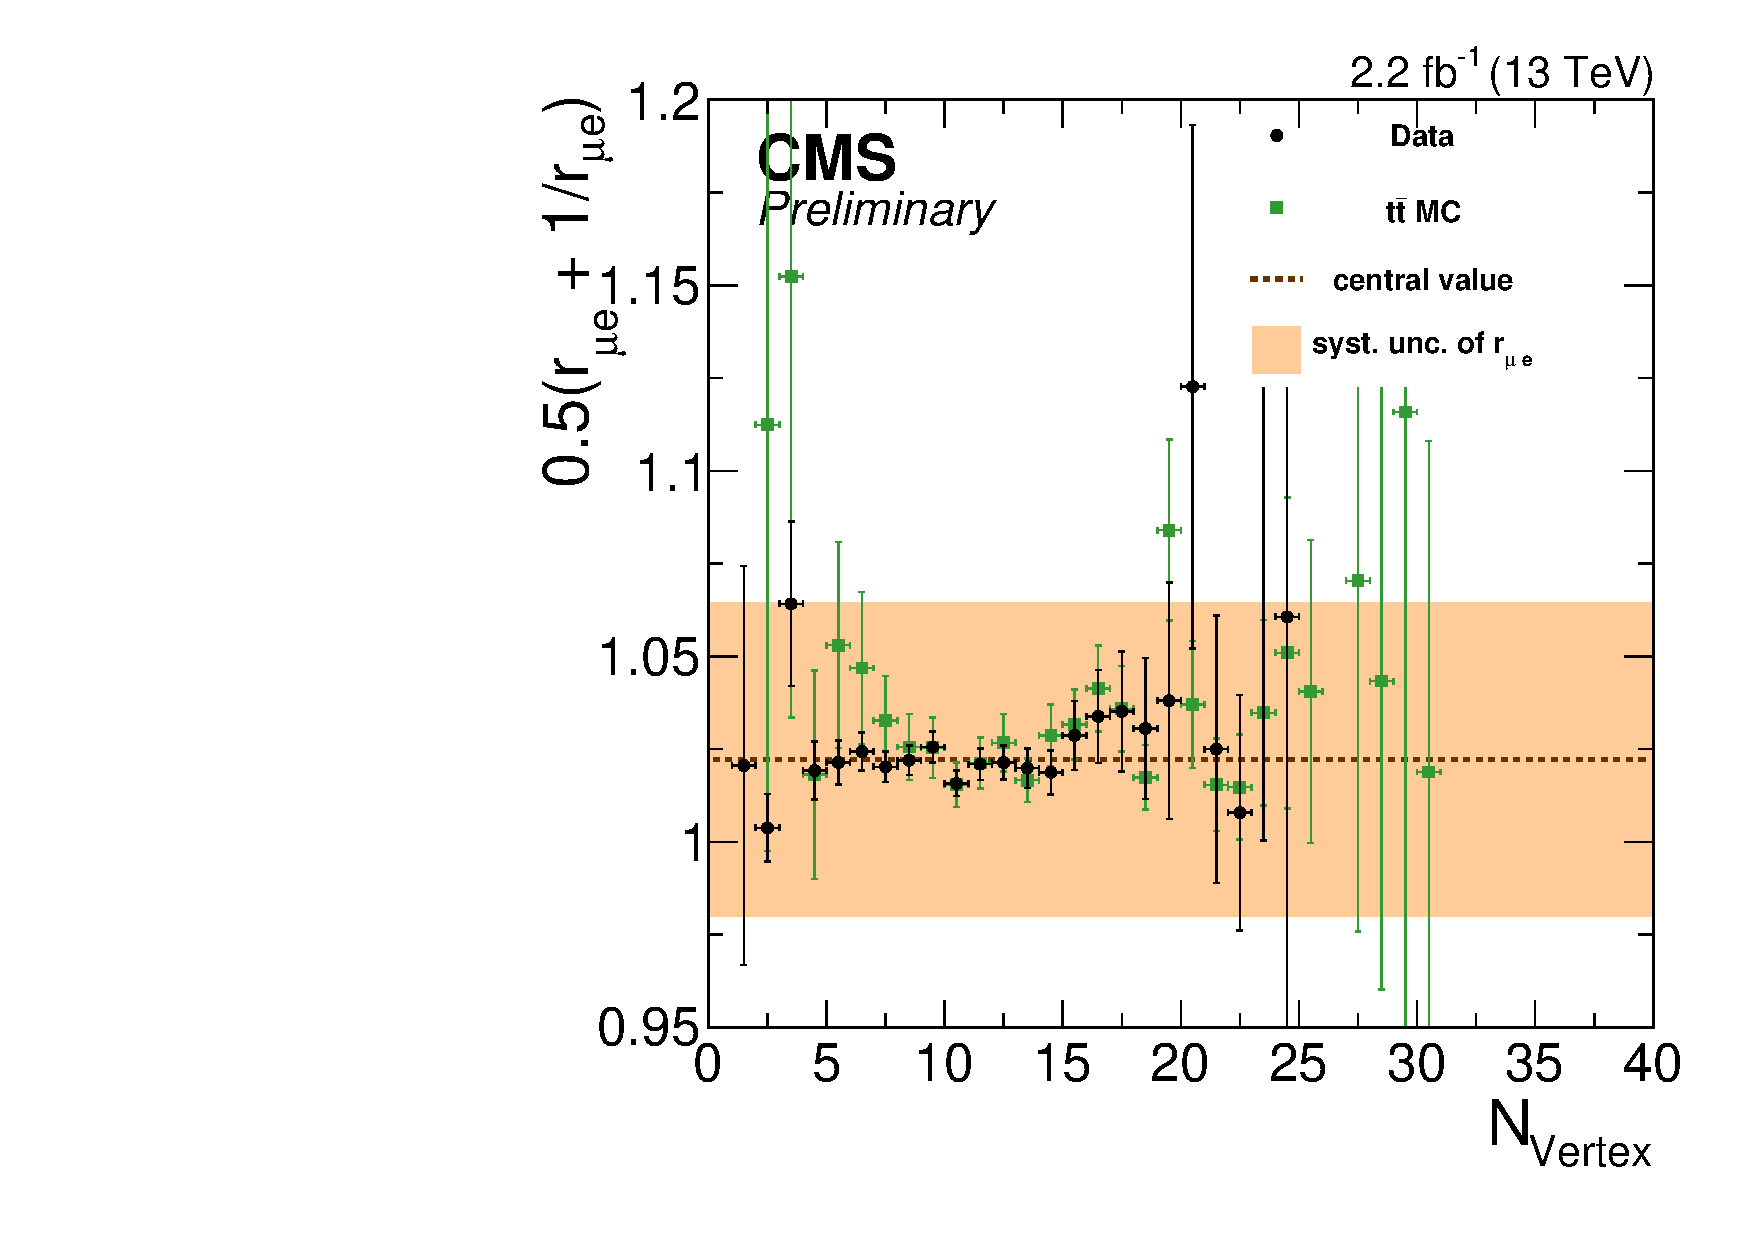
\includegraphics[width=0.30\textwidth]{bkgd/figs/rSFOFFromRMuE_ZPeakControlForward_Run2015_25ns_nVtx_None.pdf}  &
      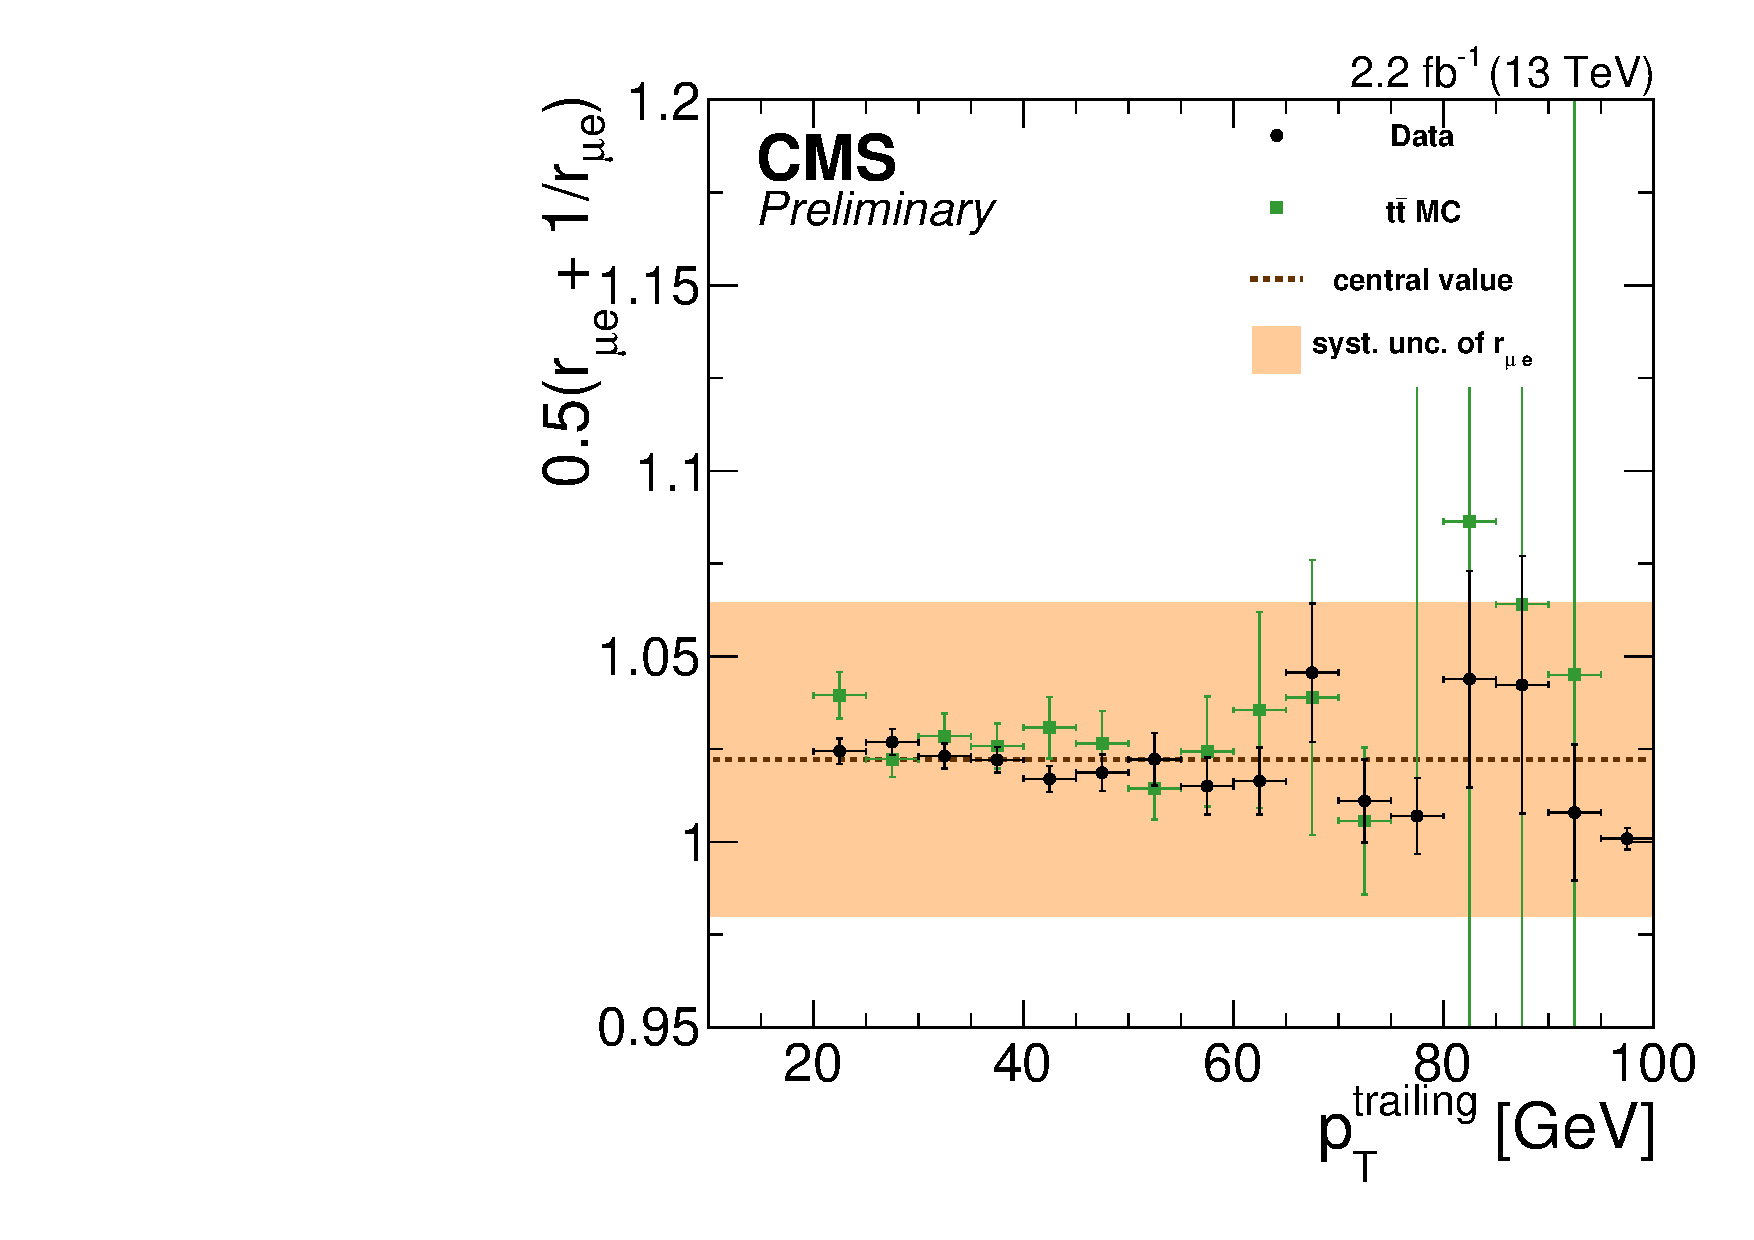
\includegraphics[width=0.30\textwidth]{bkgd/figs/rSFOFFromRMuE_ZPeakControlForward_Run2015_25ns_TrailingPt_None.pdf} \\
      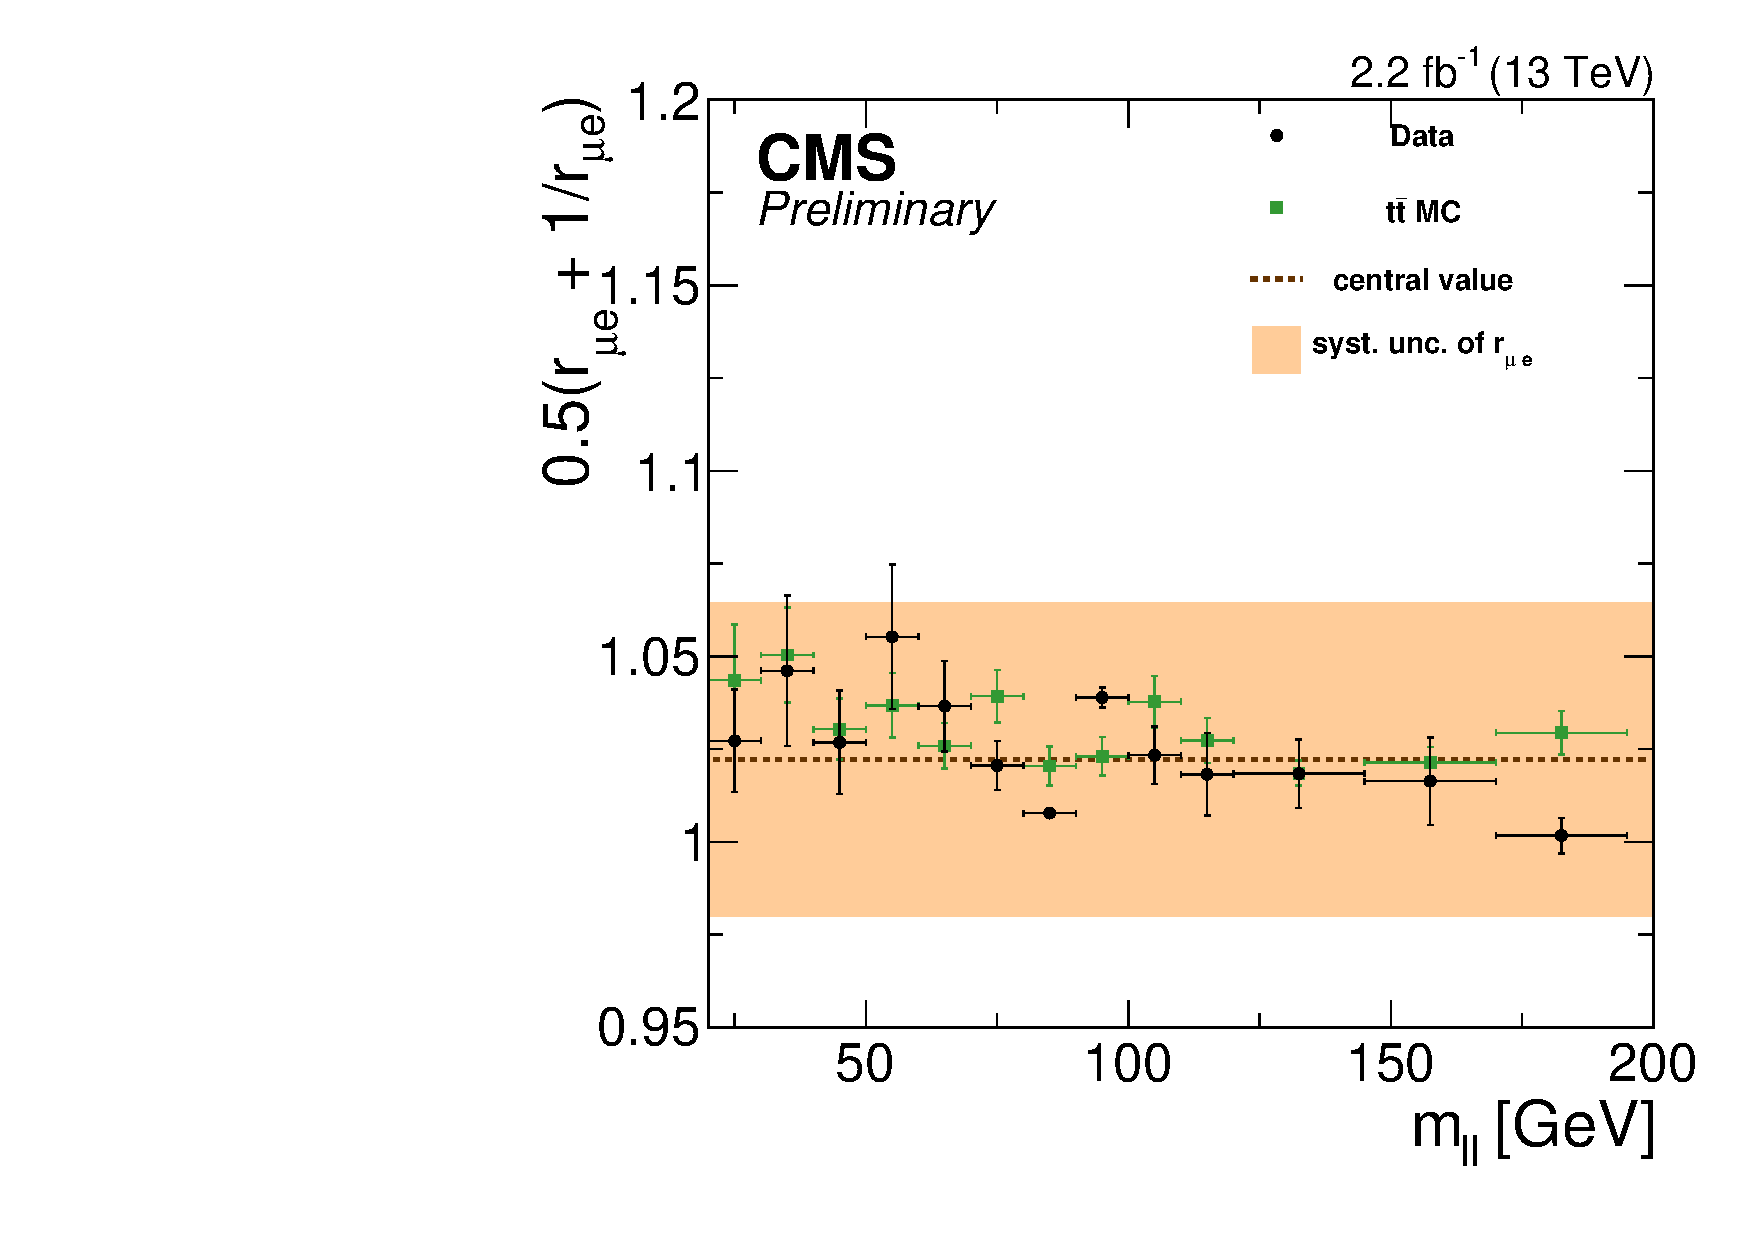
\includegraphics[width=0.30\textwidth]{bkgd/figs/rSFOFFromRMuE_ZPeakControlForward_Run2015_25ns_Mll_None.pdf} &
      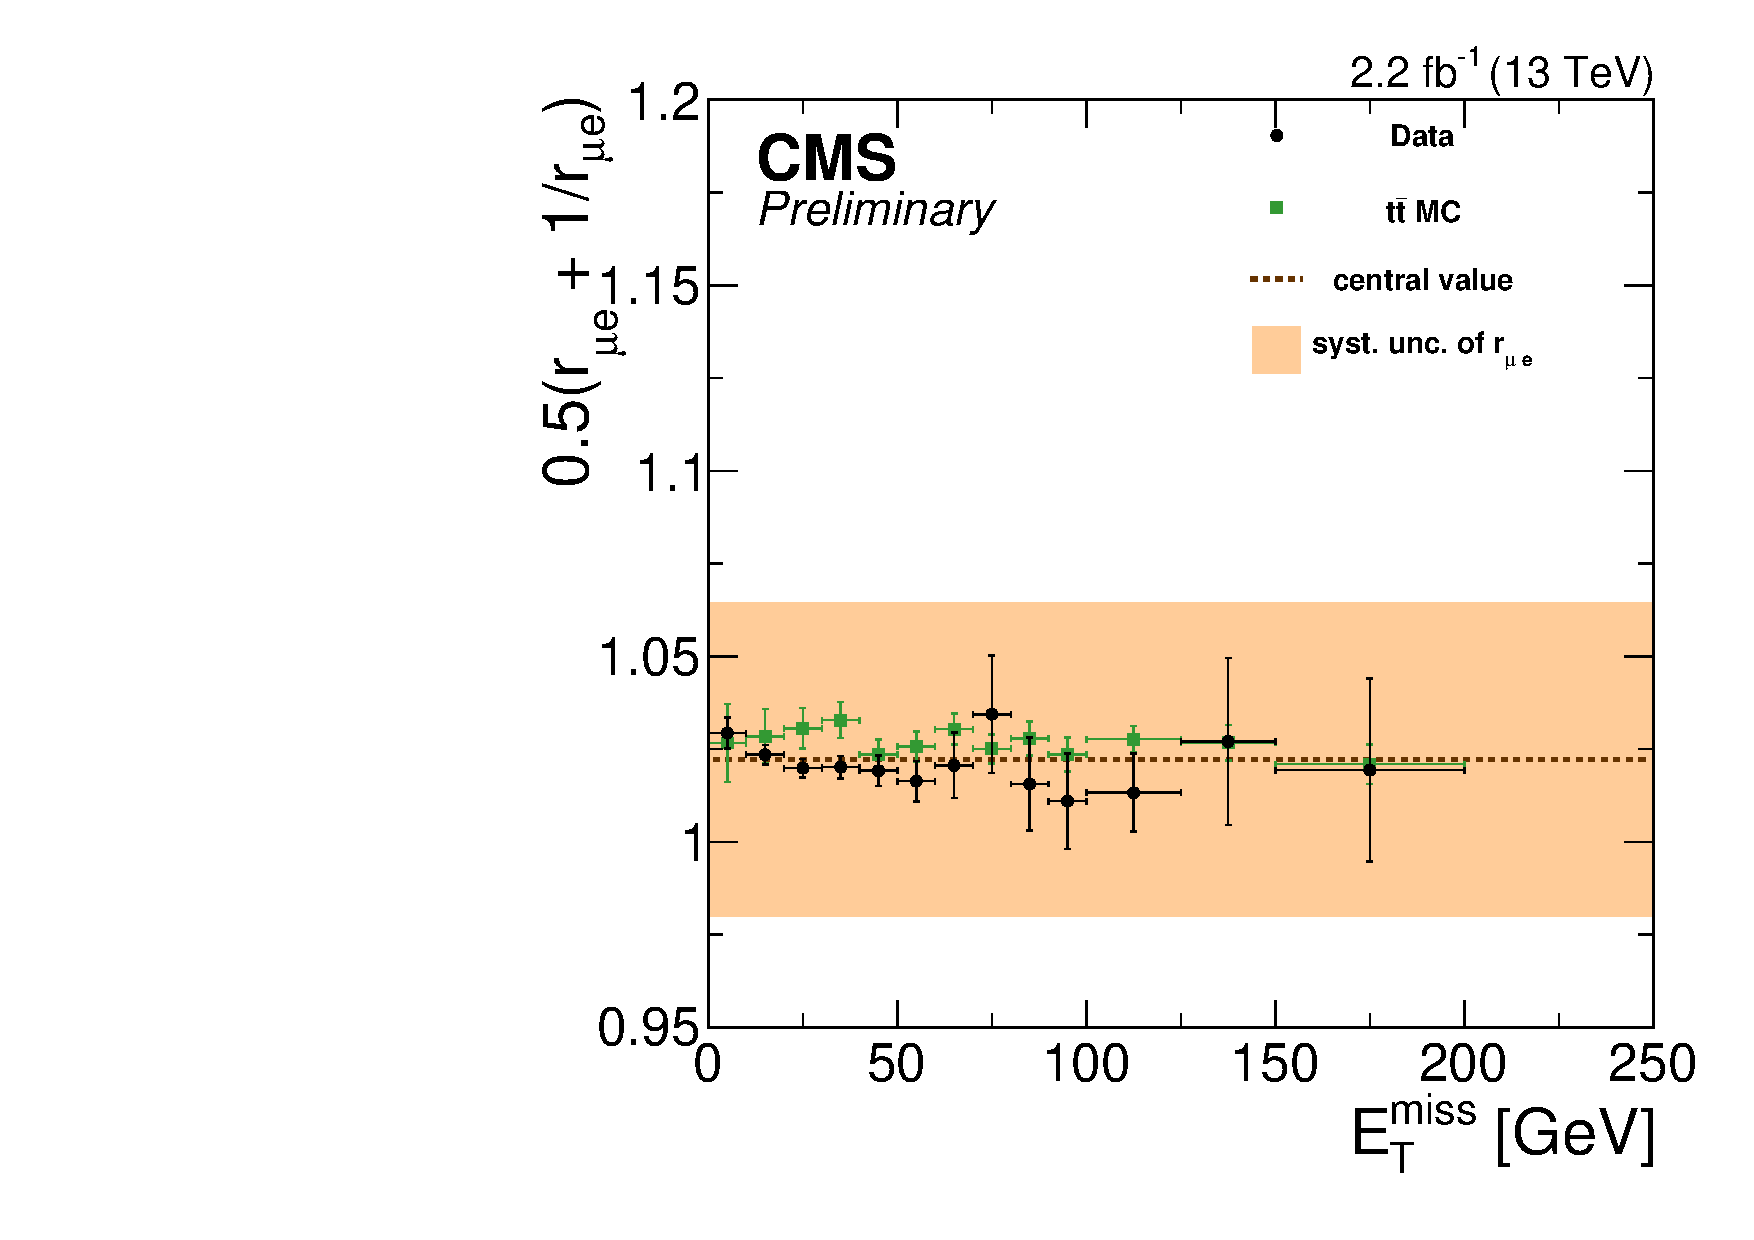
\includegraphics[width=0.30\textwidth]{bkgd/figs/rSFOFFromRMuE_ZPeakControlForward_Run2015_25ns_MET_None.pdf} &
      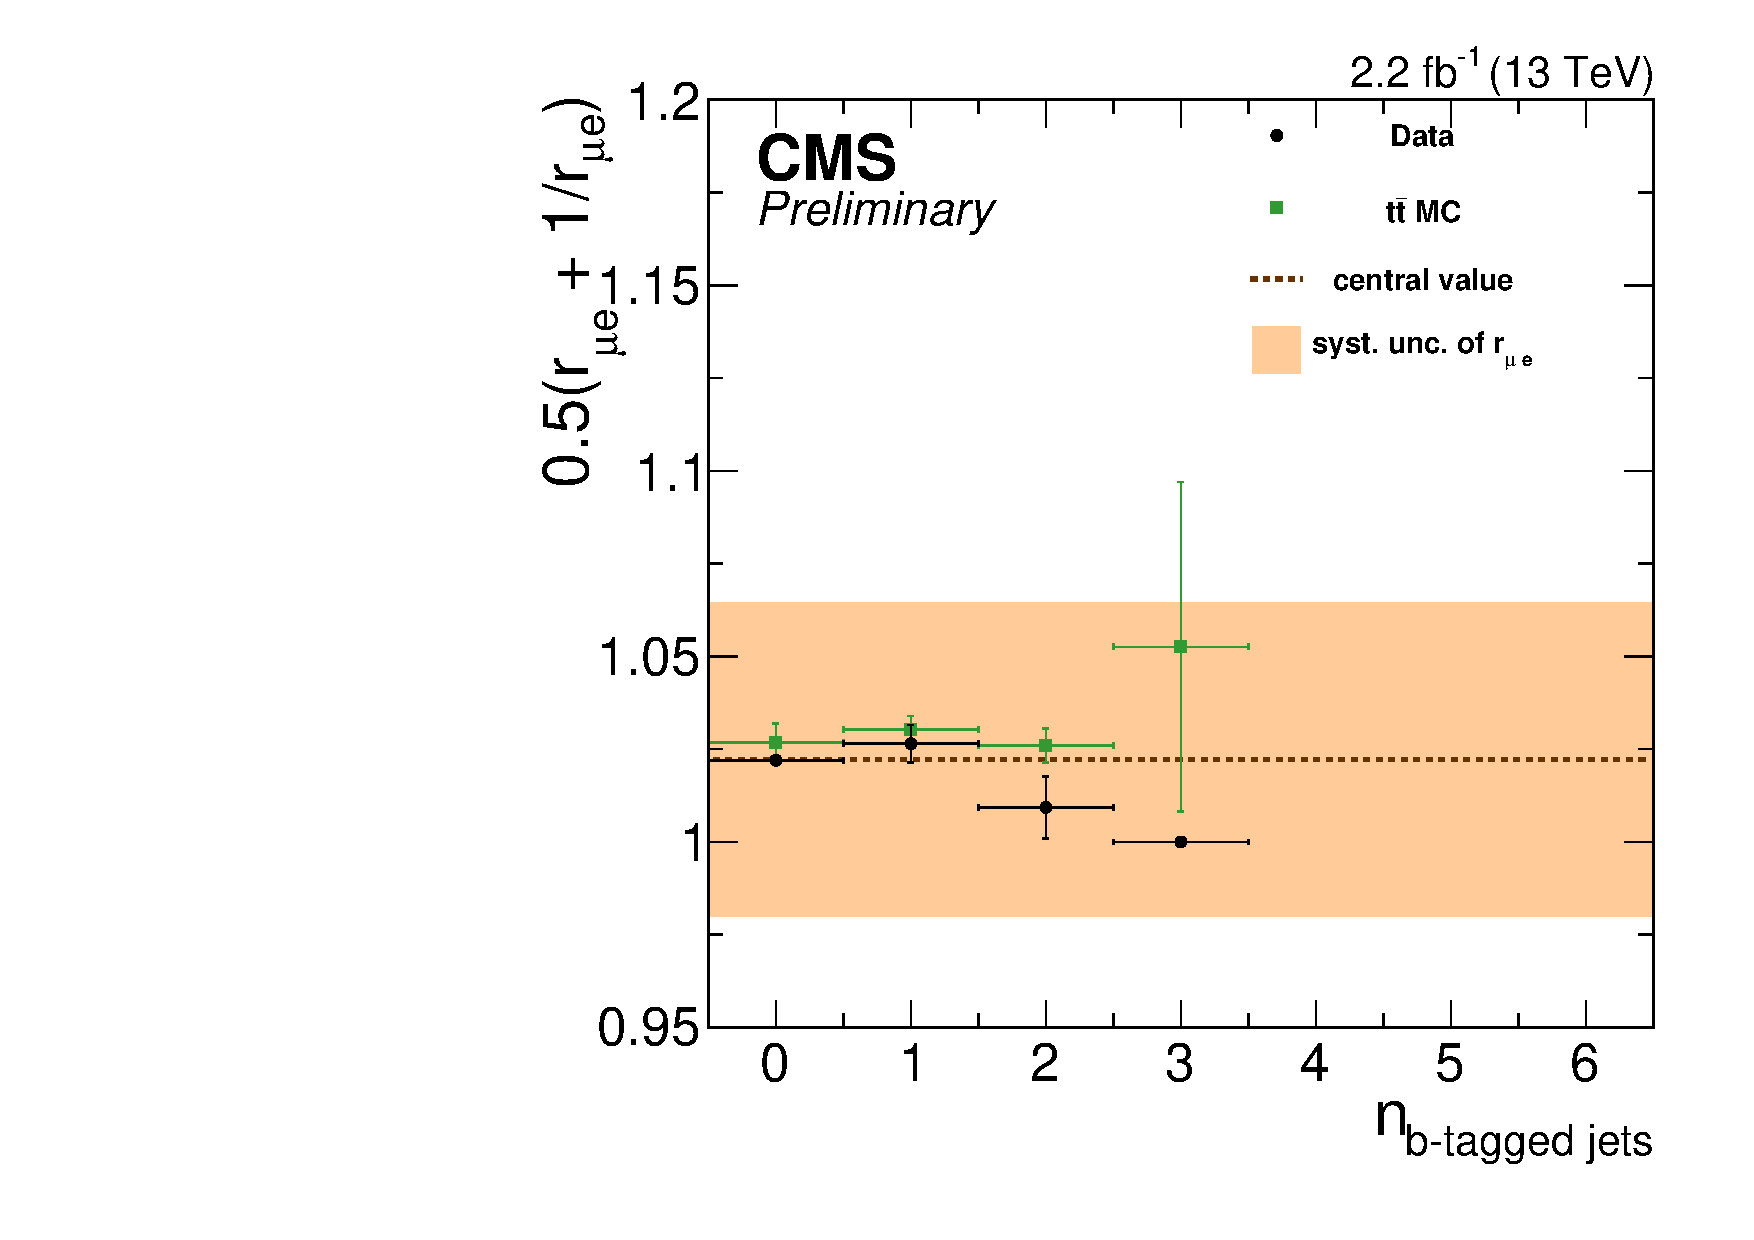
\includegraphics[width=0.30\textwidth]{bkgd/figs/rSFOFFromRMuE_ZPeakControlForward_Run2015_25ns_NBJets_None.pdf} \\
    \end{tabular}
  \end{center}
  \caption{
    \label{fig:RDependencyForward}
    0.5($r_{\mu e}+1/r_{\mu e}$) dependency for forward leptons shown as a function of \nj, \nvtx, lepton \pt, \mll, \MET, and $N_{b-tags}$.
    The uncertainty due to the assigned 20\% systematic uncertainty on \rmue~is indicated by the orange band.
  }
\end{figure}

The measurement of \rt\ is done in the following way.
First, trigger efficiencies are measured using a control sample of dilepton events,
collected with the Particle Flow HT triggers with thresholds between 200\GeV and 900\GeV\ listed in table~\ref{table:triggers}.
The efficiency is calculated as the fraction of events in this sample that also passes the dilepton triggers for the given flavor combintation as shown in equation~\ref{eqn:trigeff}.

\begin{equation}
\label{eqn:trigeff}
  \epsilon_{trigger} =\frac{\text{Lepton pair }\cap PFH_T \text{ trigger } \cap\text{ Dilepton trigger}  }{\text{Lepton pair }\cap PFH_T \text{ trigger }}
\end{equation} 

It is required that all events with \nj $\geq$ 2 and \MET $>$ 100\GeV are vetoed to exclude the signal region
and ensure the orthogonality of the factorization method and the direct measurement of \rsfof in the control region.
A minimum \HT value of 400\GeV is required to keep the PFHT triggers efficient.
This is motivated in Fig.~\ref{fig:triggerBias},
where the ratio between the measured and the true efficiencies in \ttbar simulation are shown as a function of \HT.
For low values of \HT, there is a significant deviation from unity,
more evident in the case of OF triggers.
The value is close to unity above $\approx$400\GeV,
indicating the abscense of bias in the trigger efficiency measurement due to the use of PF-\HT triggers.
It is important to note that the lowest \HT threshold included in the trigger simulation is 350\GeV.
Therefore a higher offline \HT threshold is needed in the case of MC to match this trigger requirement. 

\begin{figure}[htb]
  \begin{center}
    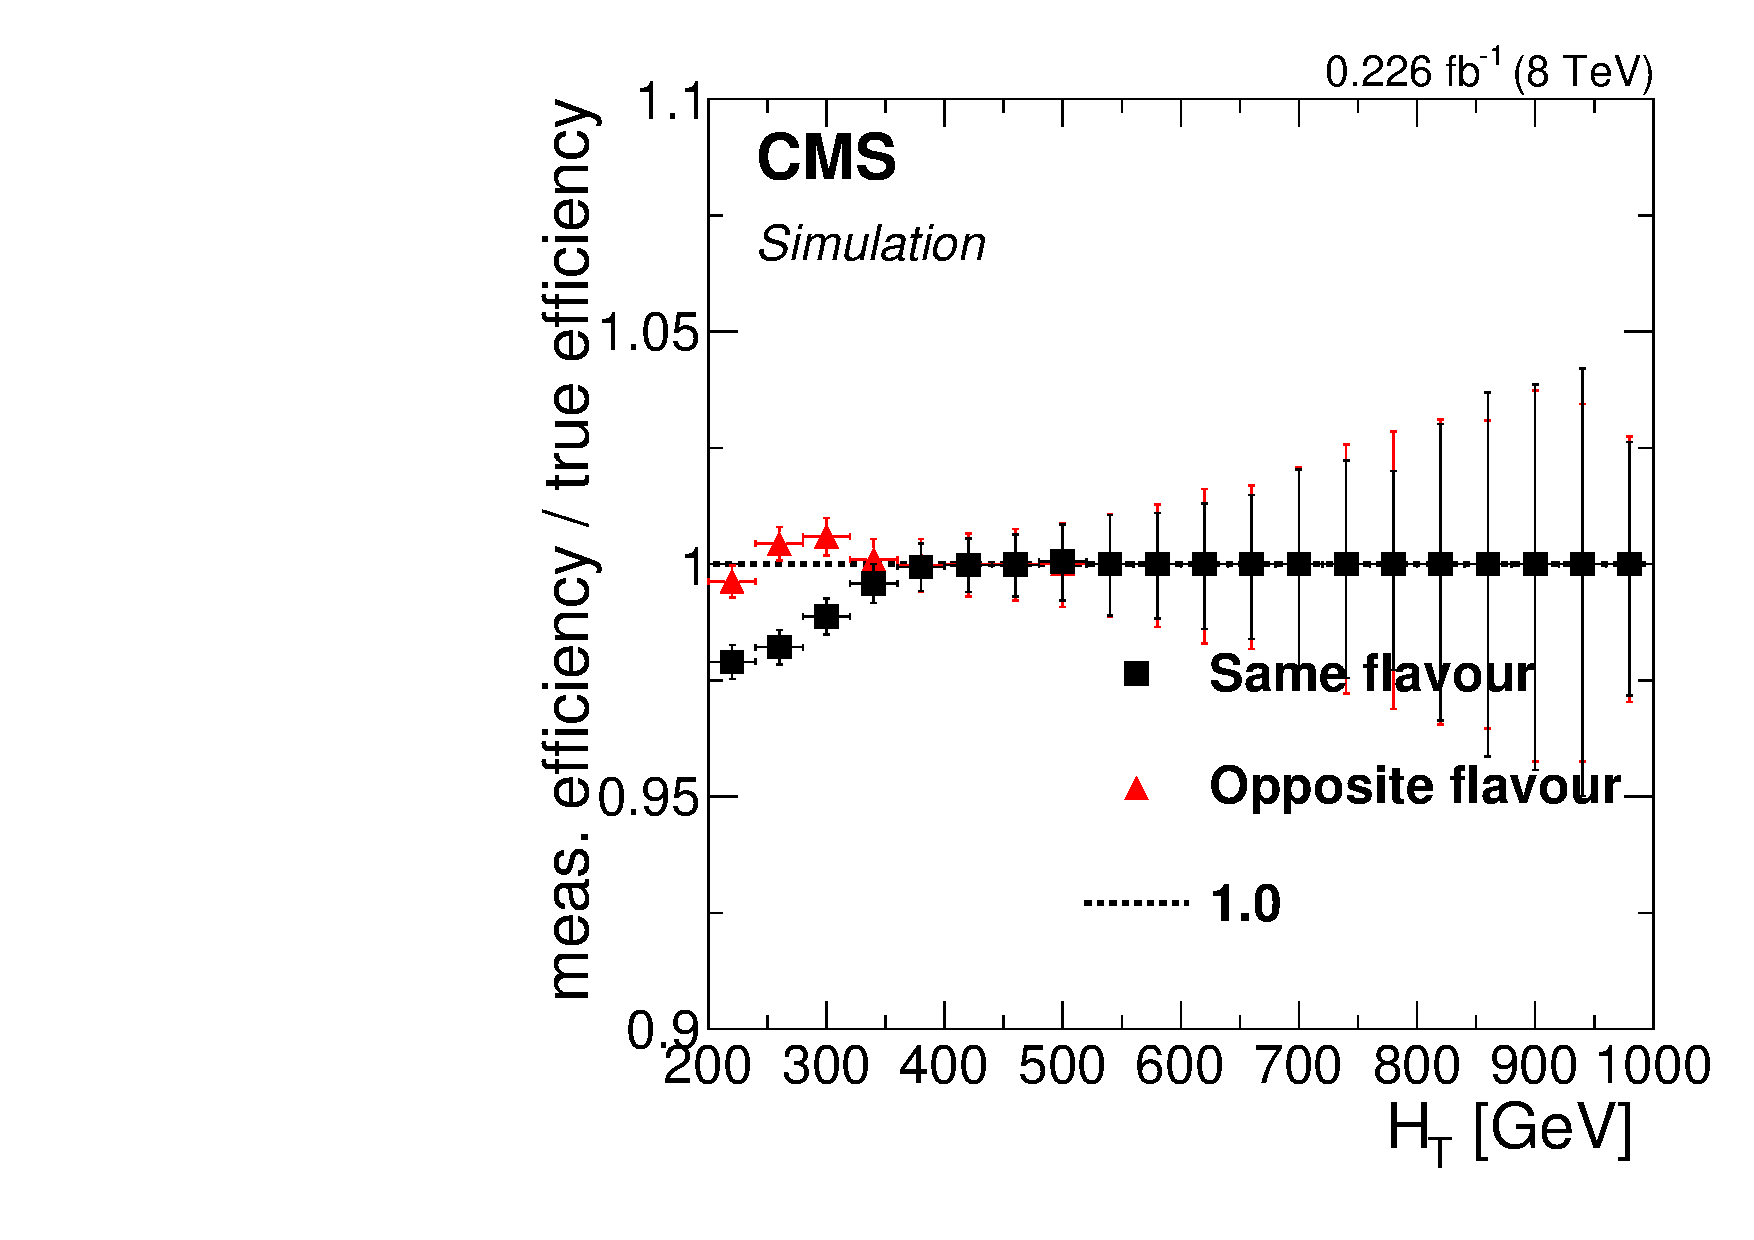
\includegraphics[scale=0.35]{bkgd/figs/Triggereff_AlphaTSyst_PFHT_HighHTExclusive_Run2015_25ns_HT_None.pdf}
    \caption{
      \label{fig:triggerBias}
      Ratio of measured to true trigger efficiency for combined SF and OF triggers as a function of \HT measured in \ttbar simulation.
      A value of 1 indicates no bias due to the choice of the supporting triggers.
    }
  \end{center}
\end{figure}

The resulting trigger efficiencies measured in data and MC ares shown in table~\ref{tab:EffValues_Seperated}.
All the trigger efficiencies are consistent with eachother in the central region,
and the e$\mu$ trigger efficiencies are measured to be slightly lower in the forward regions.
The values measured in data are limited by statistics, but the values measured are consistent with the values measured in MC.

\begin{table}[hbp]
  \begin{center}
  \caption{
    Trigger efficiencies for data and MC with OS, $p_T>20(20)\,\GeV$
    and $H_T>400\,\GeV$ for central and forward region seperated.
  } 
  \begin{tabular}{l|c|c|c}     
    & numerator & denominator & $\epsilon_{trigger} \pm \sigma_{stat}$  \\ 
    \hline
    &\multicolumn{3}{c}{Data} \\
    \hline
    &  \multicolumn{3}{|c}{ Central } \\
    \hline
    ee       & 837 & 885 & 0.95$\pm$0.01  \\
    $\mu\mu$ & 430 & 462 & 0.93$\pm$0.01  \\
    e$\mu$   & 160 & 171 & 0.94$\pm$0.03  \\        
    \hline 
    &  \multicolumn{3}{|c}{ Forward } \\
    \hline
    ee       & 285 & 297 & 0.96$\pm$0.02  \\
    $\mu\mu$ & 226 & 244 & 0.93$\pm$0.02  \\
    e$\mu$   &  64 &  72 & 0.89$\pm$0.05  \\
    \hline
    \hline
    & \multicolumn{3}{c}{MC} \\
    \hline
    & \multicolumn{3}{|c}{ Central } \\
    \hline 
    ee       &  982.3 & 1041.5 & 0.943$\pm$0.001 \\
    $\mu\mu$ &  623.0 &  664.1 & 0.938$\pm$0.002 \\
    e$\mu$   & 1763.7 & 1926.1 & 0.916$\pm$0.001 \\    
    \hline 
    & \multicolumn{3}{|c}{ Forward } \\
    \hline 
    ee       &  363.3 & 390.8 & 0.930$\pm$0.003 \\
    $\mu\mu$ &  284.7 & 307.2 & 0.927$\pm$0.003 \\
    e$\mu$   &  720.4 & 798.9 & 0.902$\pm$0.002 \\    
    \hline 
    \hline
  \end{tabular}  
  \label{tab:EffValues_Seperated}
  \end{center}
\end{table}	

Similarliy to \rmue, the dependency of \rt on different observables is studied.
The results are shown in figures~\ref{fig:EffDependencyBarrel} and~\ref{fig:EffDependencyEndcap}.
No significant dependency of \rt on any event property is observed,
and a systematic uncertainty of 5\% is assigned to each of the trigger efficiencies,
which translates to an uncertainty of 6\% on \rt.

\begin{figure}[htb]
  \begin{center}
    \begin{tabular}{ccc}
      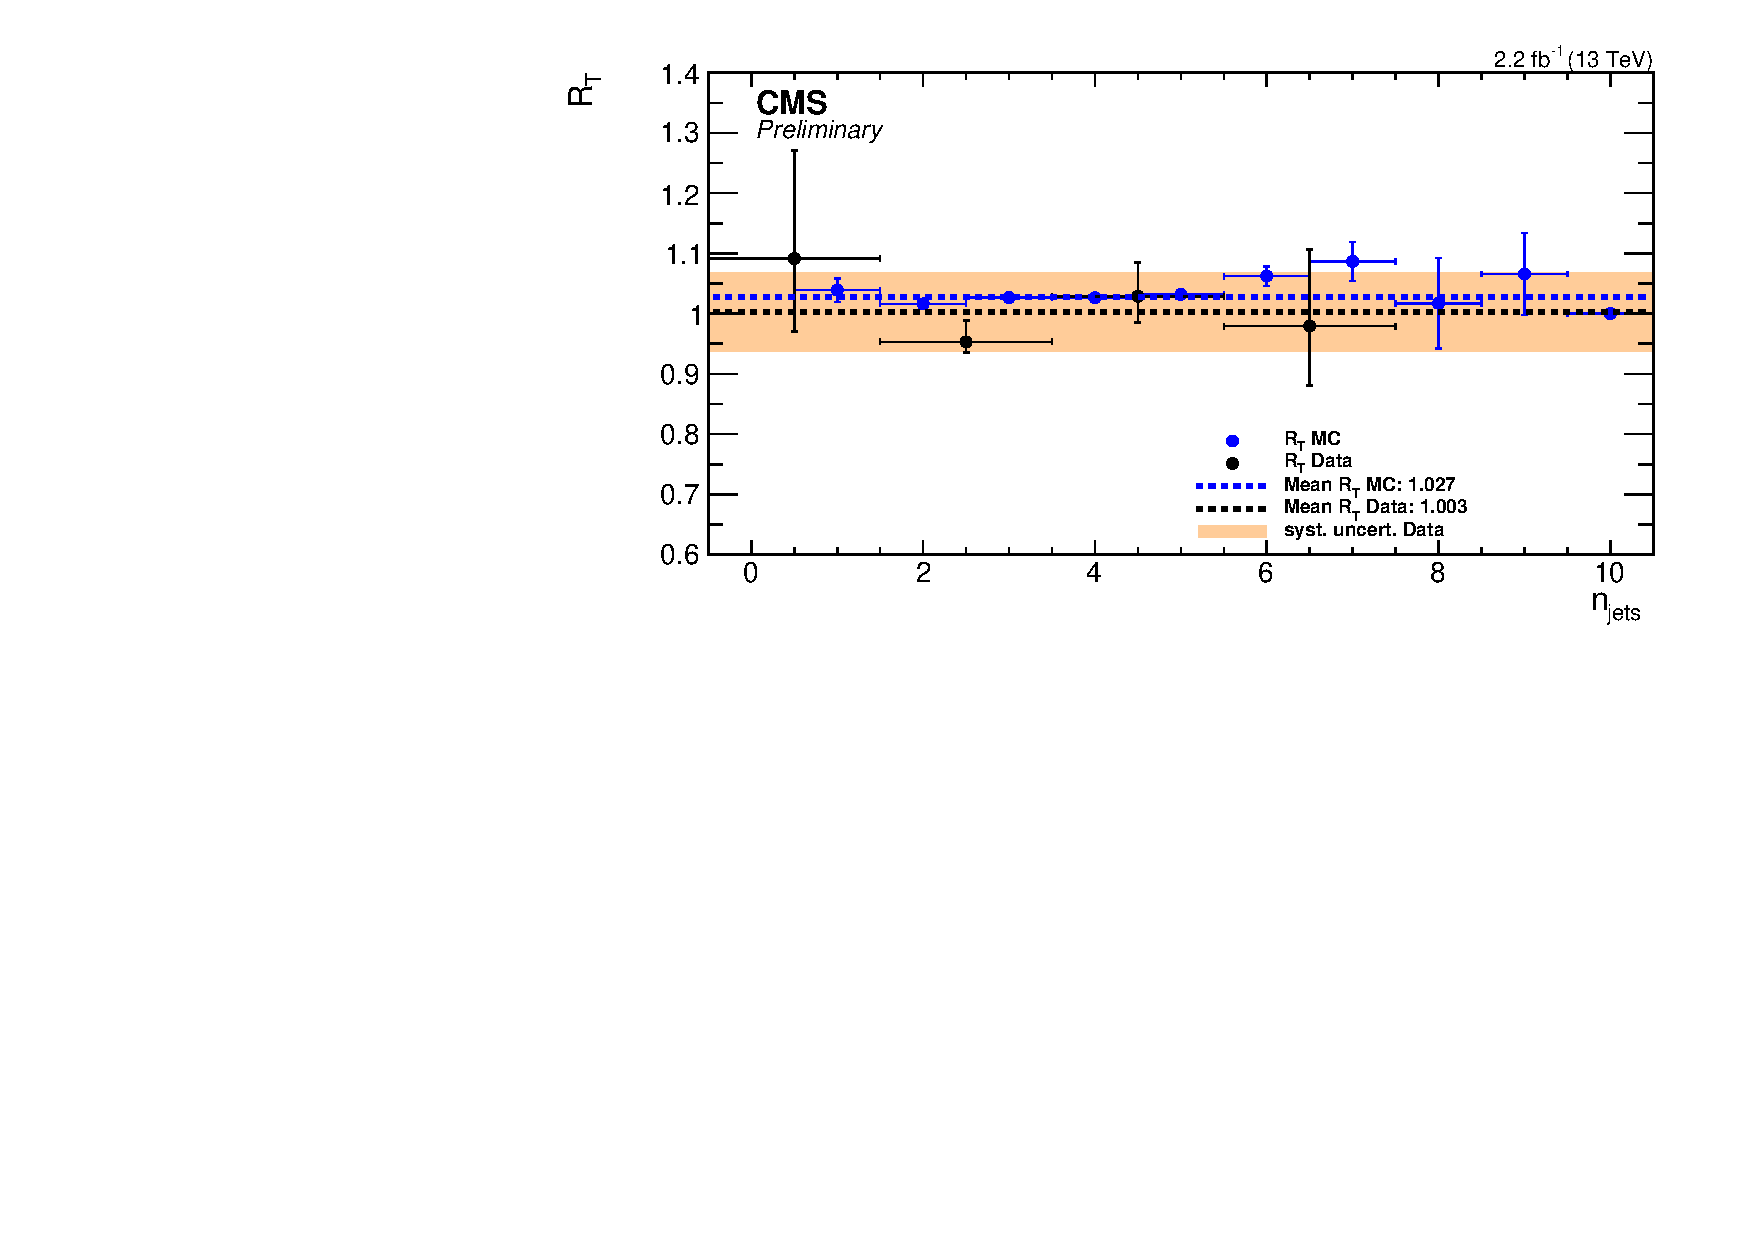
\includegraphics[width=0.30\textwidth]{bkgd/figs/Triggereff_SFvsOF_Syst_PFHT_HighHTExclusiveCentral_Run2015_25ns_NJets_None_NonIso_MC.pdf} &
      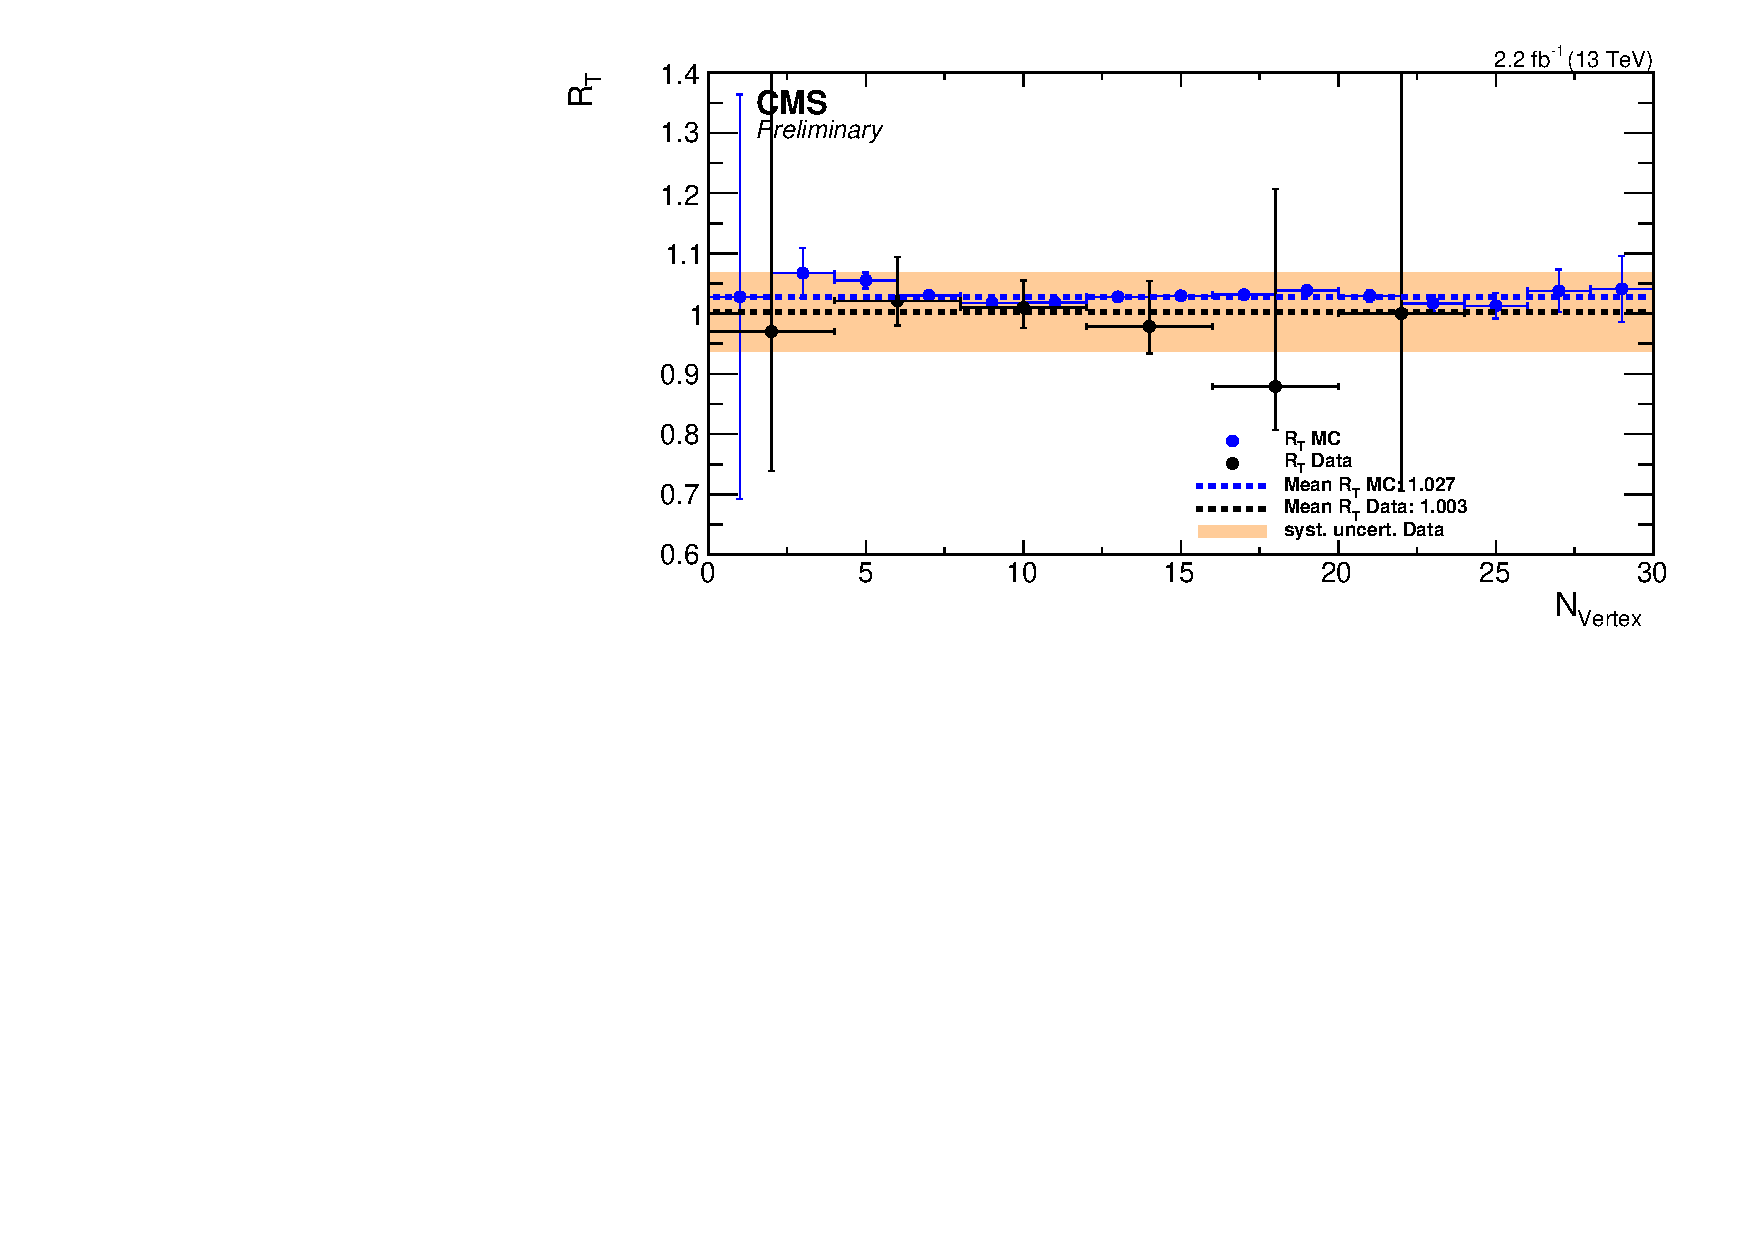
\includegraphics[width=0.30\textwidth]{bkgd/figs/Triggereff_SFvsOF_Syst_PFHT_HighHTExclusiveCentral_Run2015_25ns_nVtx_None_NonIso_MC.pdf}  &
      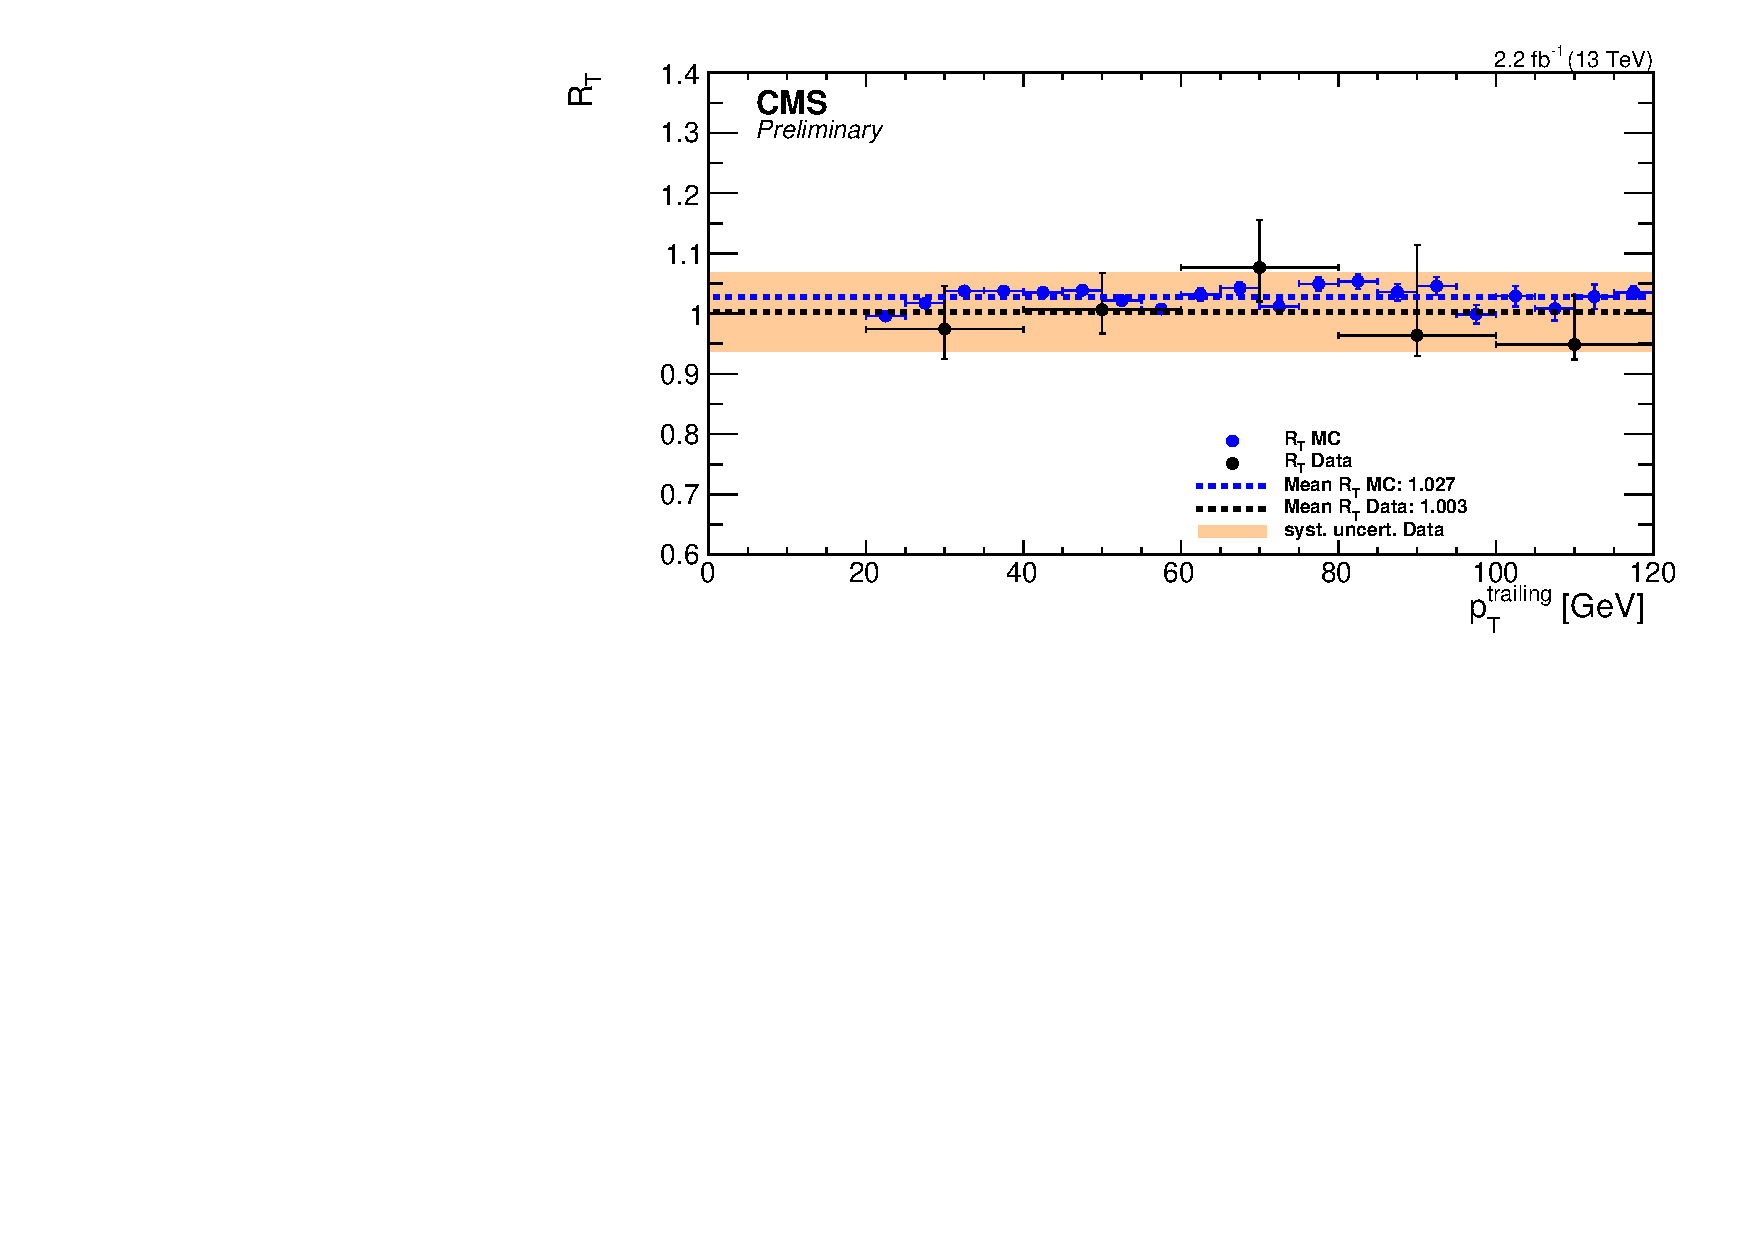
\includegraphics[width=0.30\textwidth]{bkgd/figs/Triggereff_SFvsOF_Syst_PFHT_HighHTExclusiveCentral_Run2015_25ns_TrailingPt_None_NonIso_MC.pdf} \\
      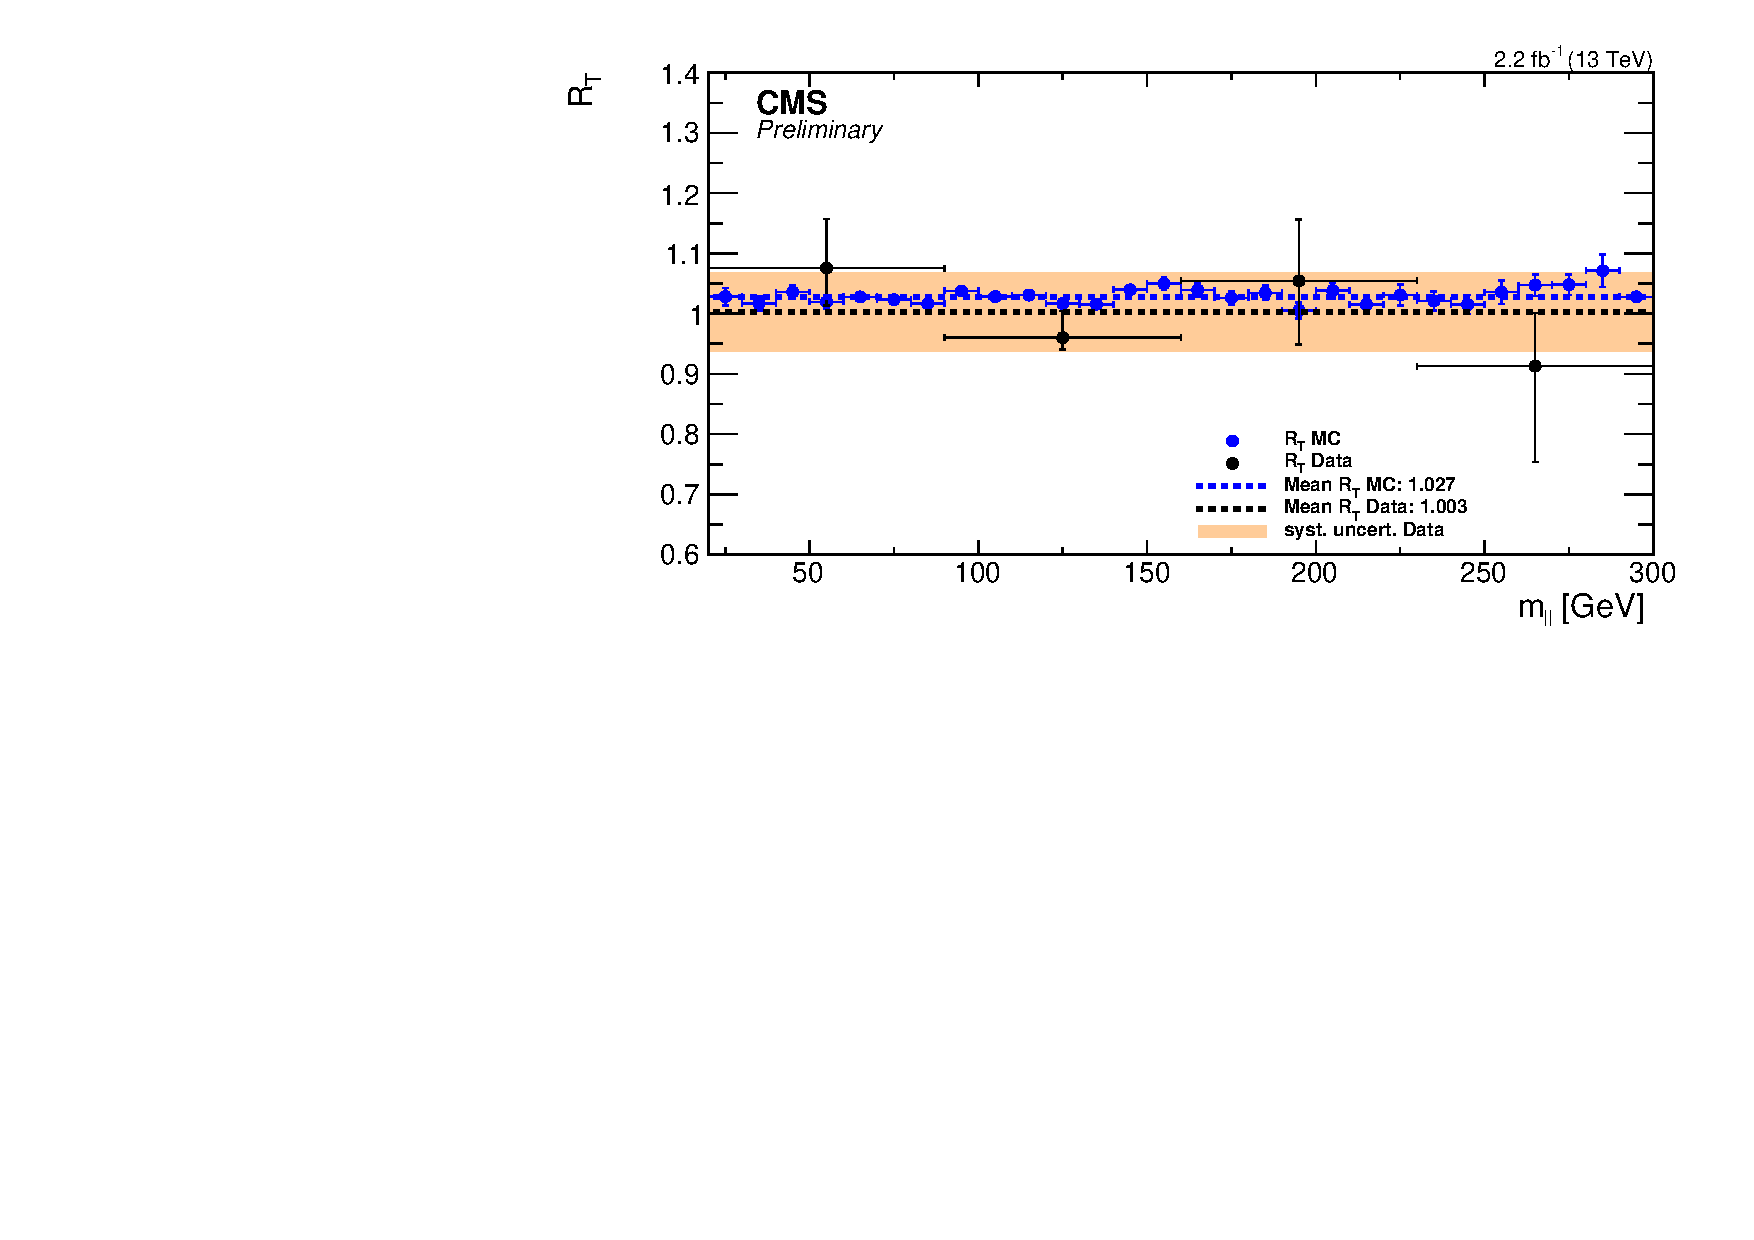
\includegraphics[width=0.30\textwidth]{bkgd/figs/Triggereff_SFvsOF_Syst_PFHT_HighHTExclusiveCentral_Run2015_25ns_Mll_None_NonIso_MC.pdf} &
      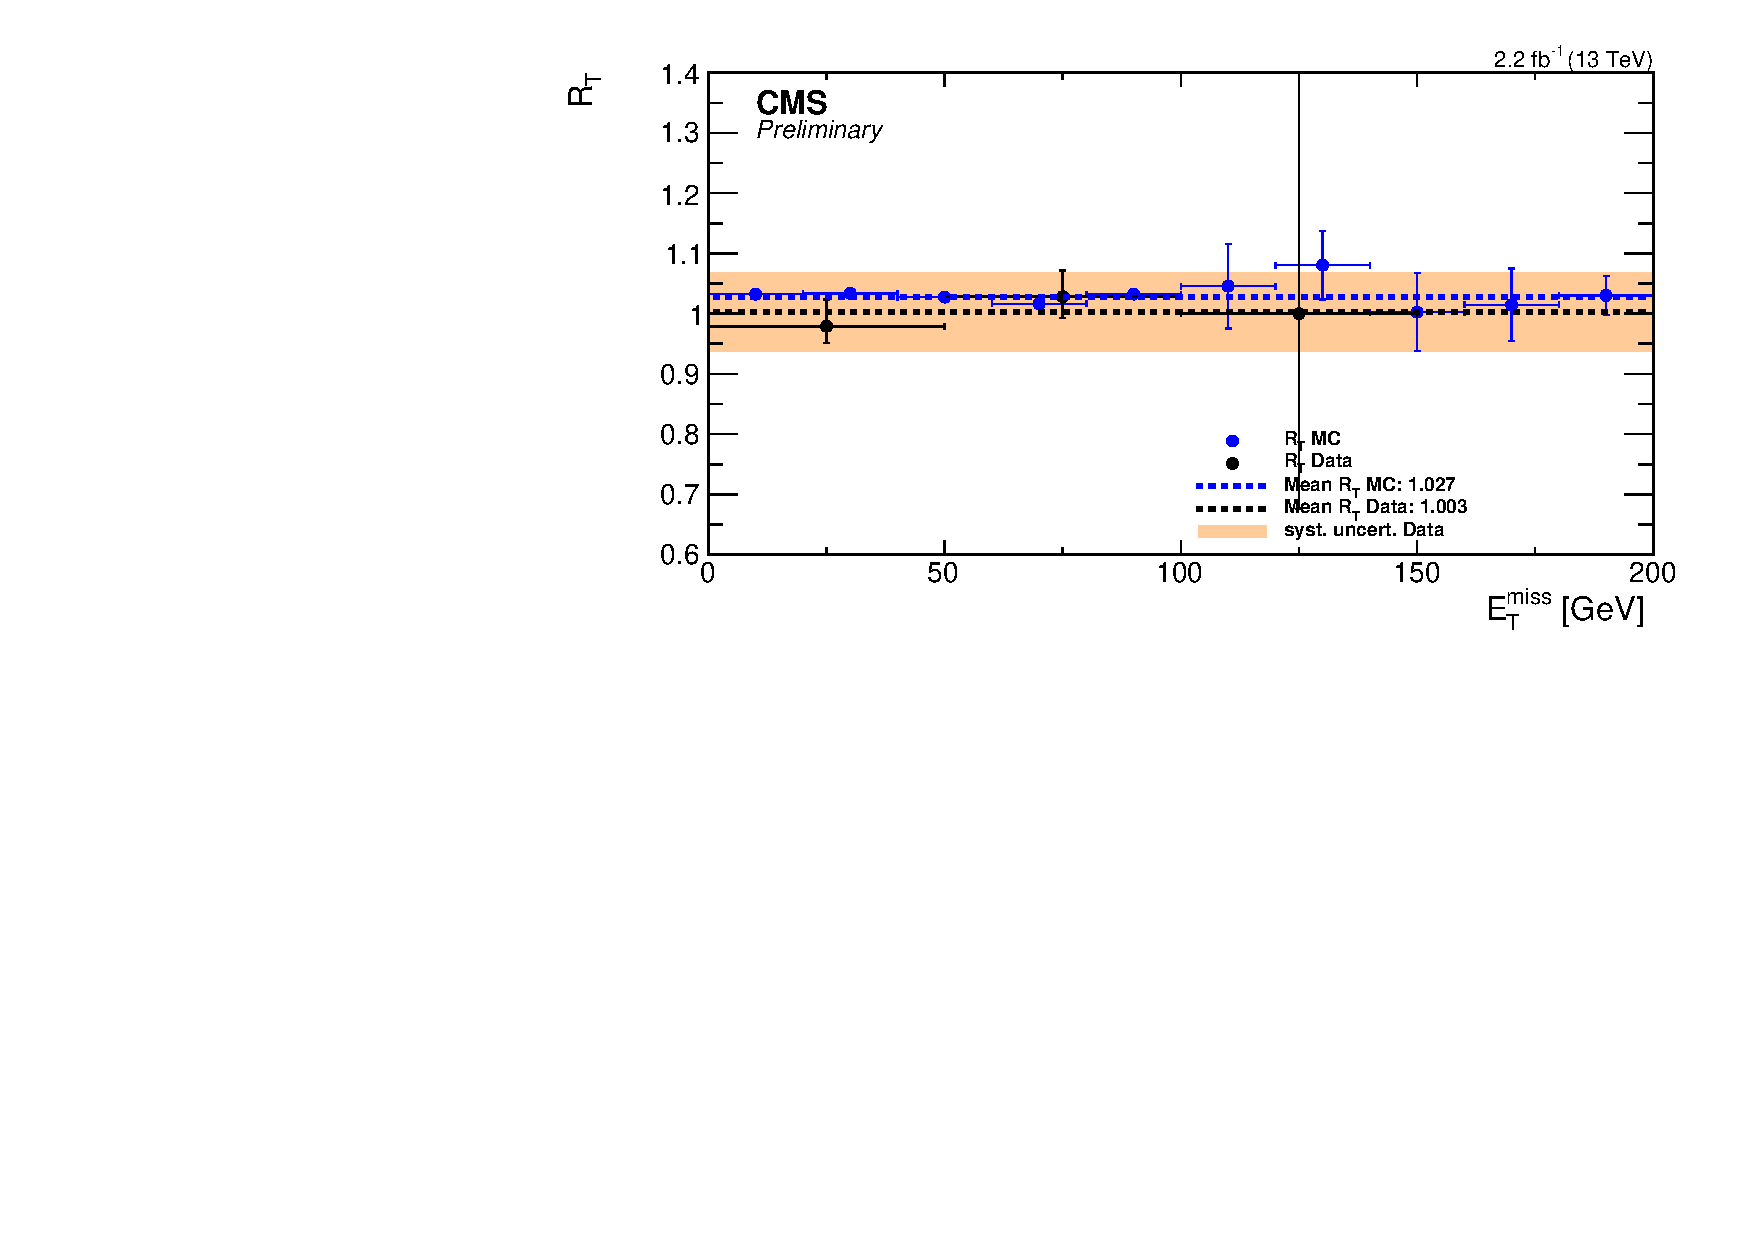
\includegraphics[width=0.30\textwidth]{bkgd/figs/Triggereff_SFvsOF_Syst_PFHT_HighHTExclusiveCentral_Run2015_25ns_MET_None_NonIso_MC.pdf} &
      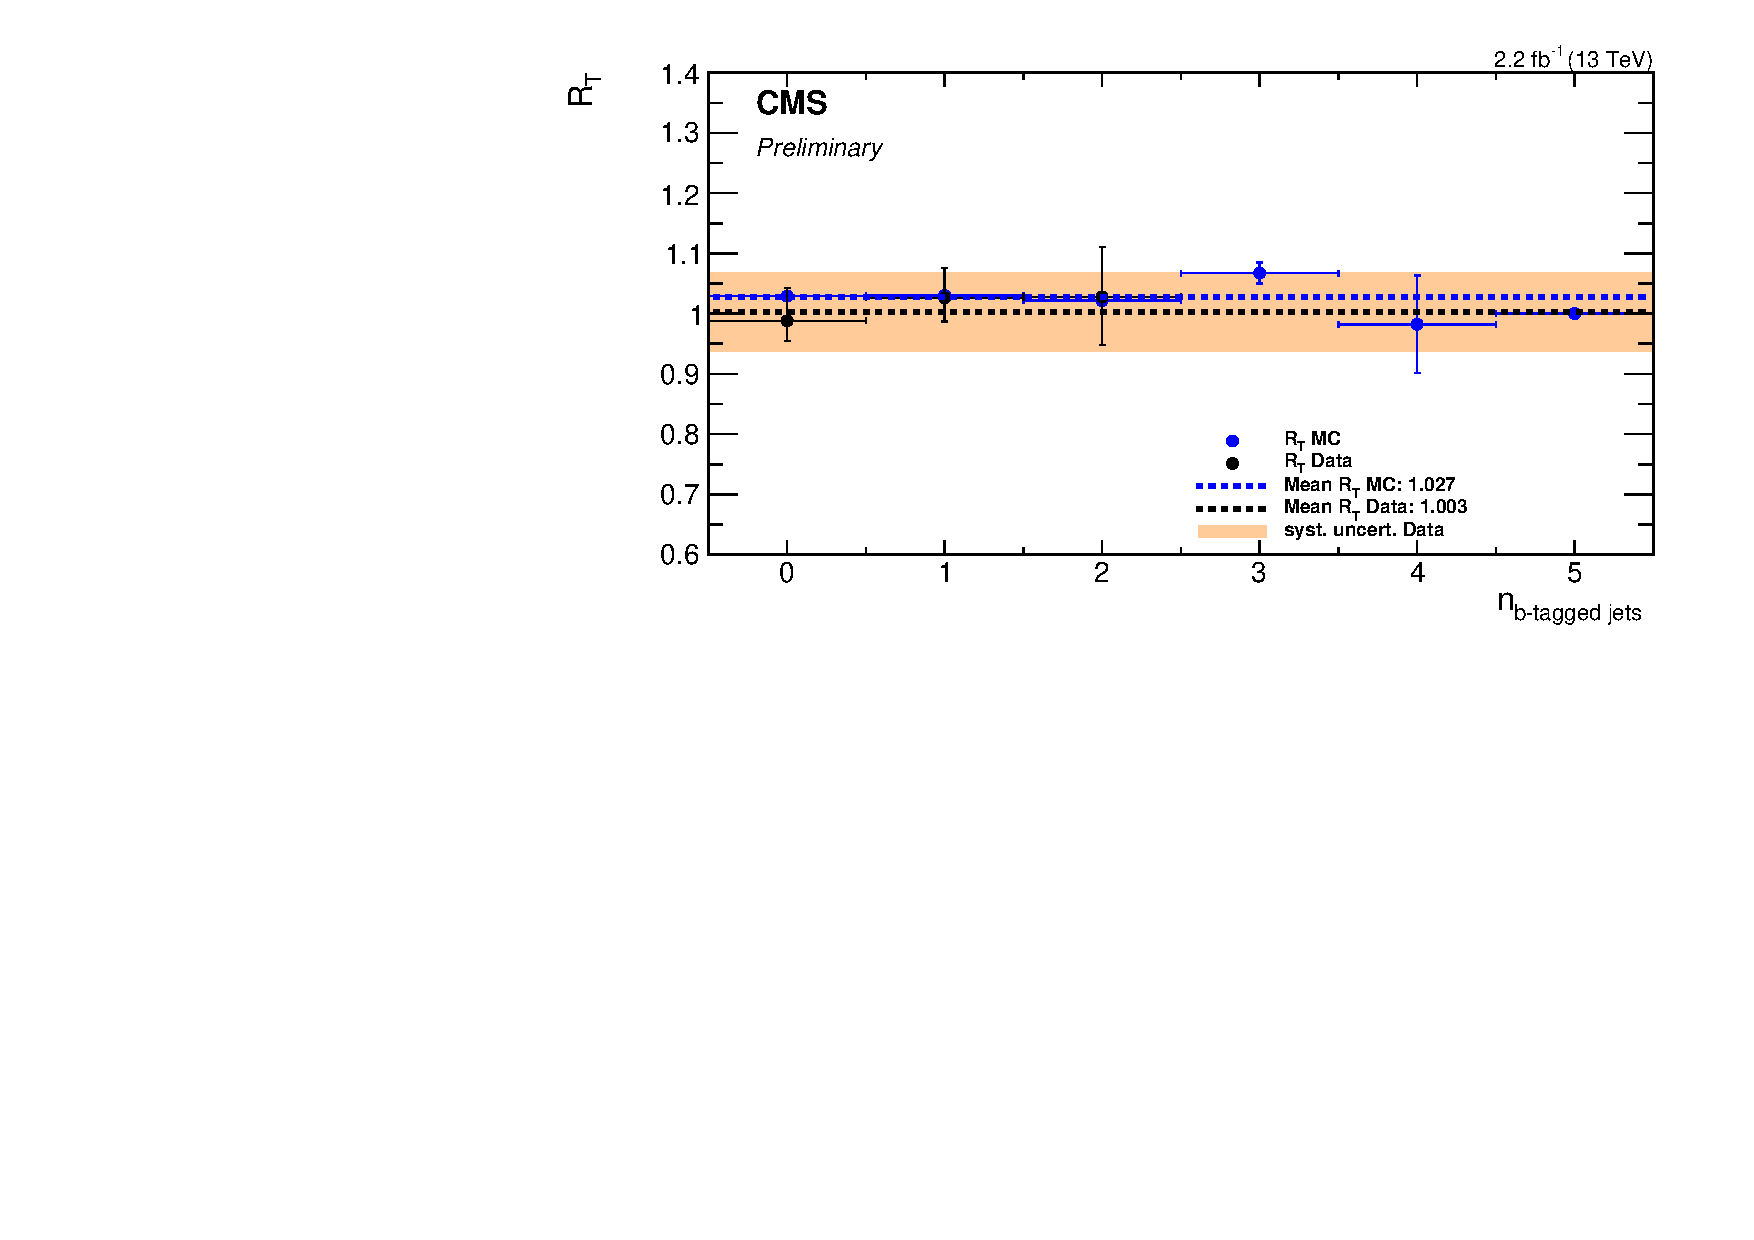
\includegraphics[width=0.30\textwidth]{bkgd/figs/Triggereff_SFvsOF_Syst_PFHT_HighHTExclusiveCentral_Run2015_25ns_NBJets_None_NonIso_MC.pdf} \\
    \end{tabular}
    \caption{
      \label{fig:EffDependencyBarrel}
      \rt\ dependency for central leptons shown as a function of \nj, \nvtx, lepton \pt, \mll, \MET, and $N_{b-tags}$.
      The assigned 6.4\% systematic uncertainty on \rt is indicated by the orange band.
    }
  \end{center}
\end{figure}

\begin{figure}[htb]
  \begin{center}
    \begin{tabular}{ccc}
      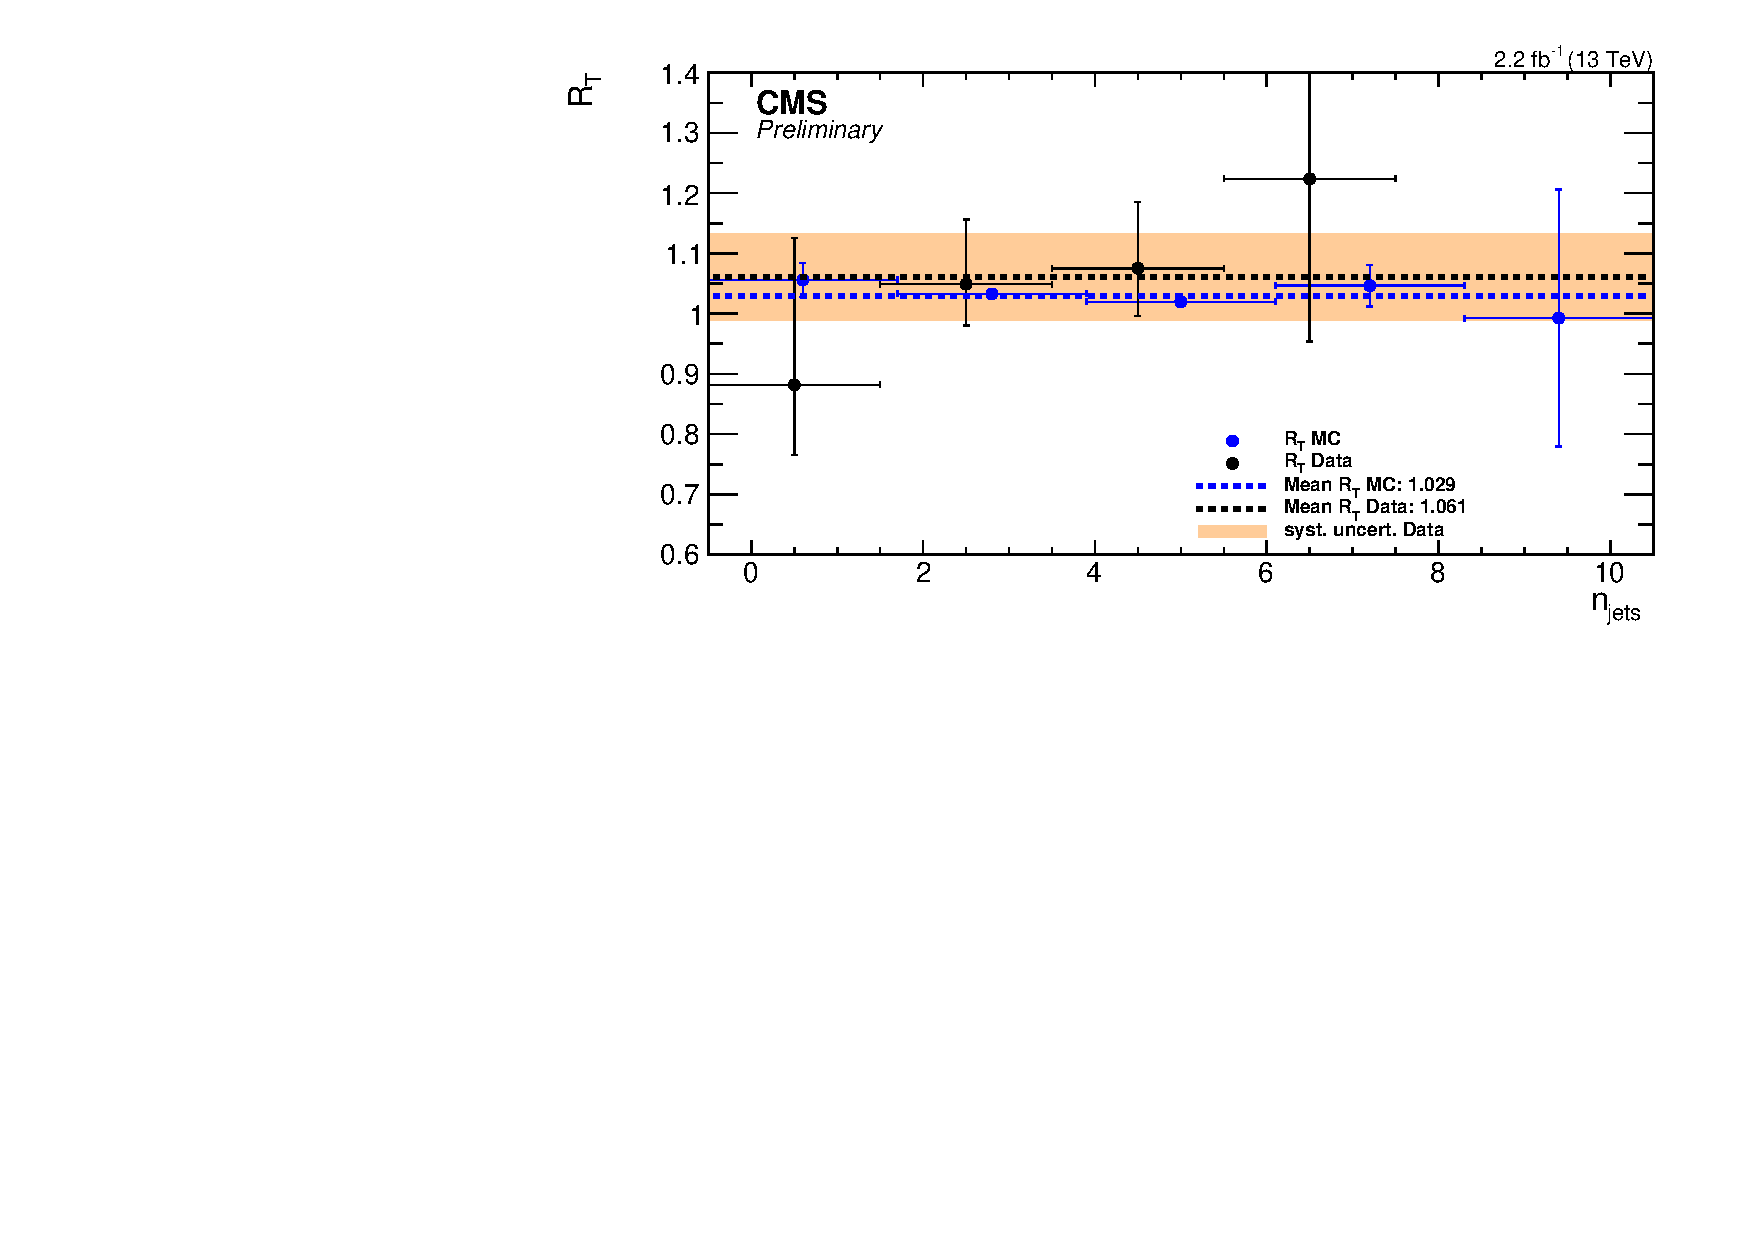
\includegraphics[width=0.30\textwidth]{bkgd/figs/Triggereff_SFvsOF_Syst_PFHT_HighHTExclusiveForward_Run2015_25ns_NJets_None_NonIso_MC.pdf} &
      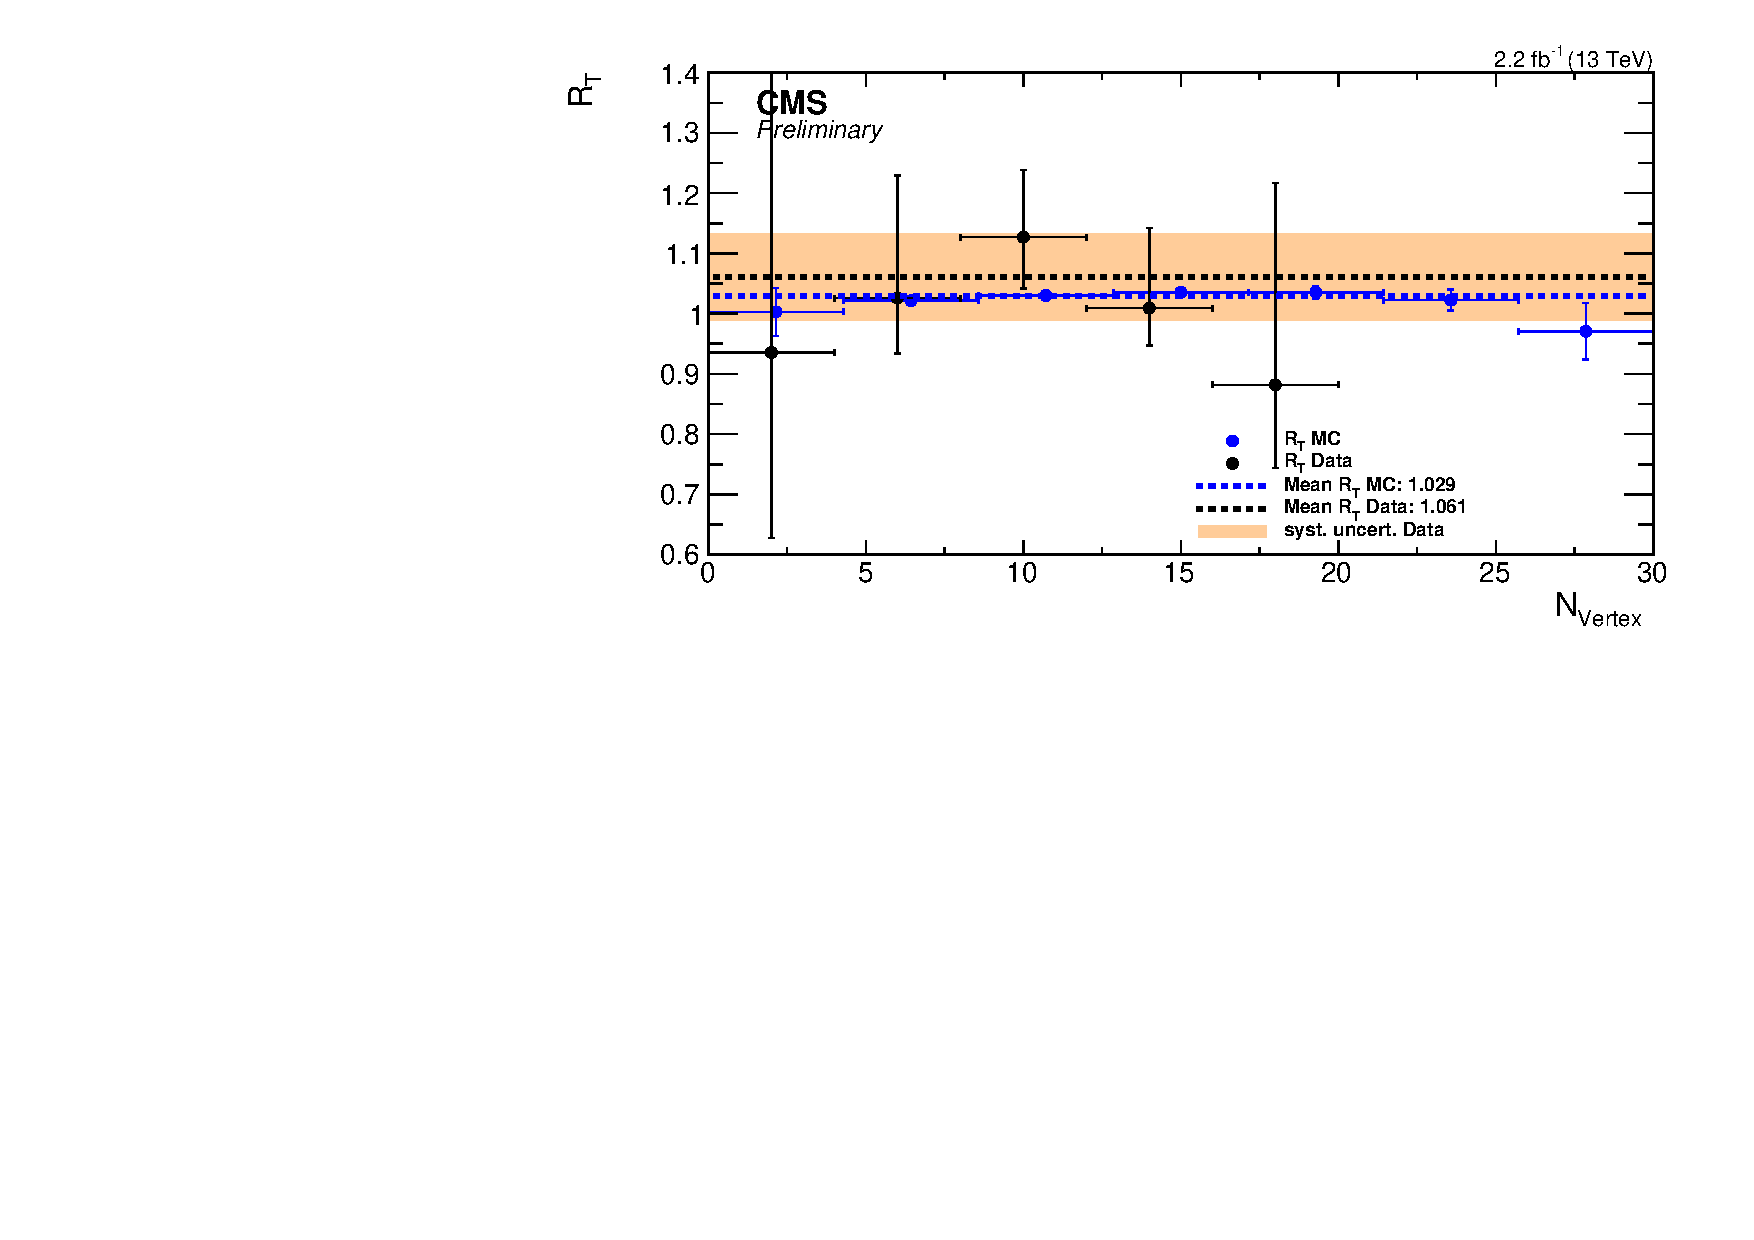
\includegraphics[width=0.30\textwidth]{bkgd/figs/Triggereff_SFvsOF_Syst_PFHT_HighHTExclusiveForward_Run2015_25ns_nVtx_None_NonIso_MC.pdf}  &
      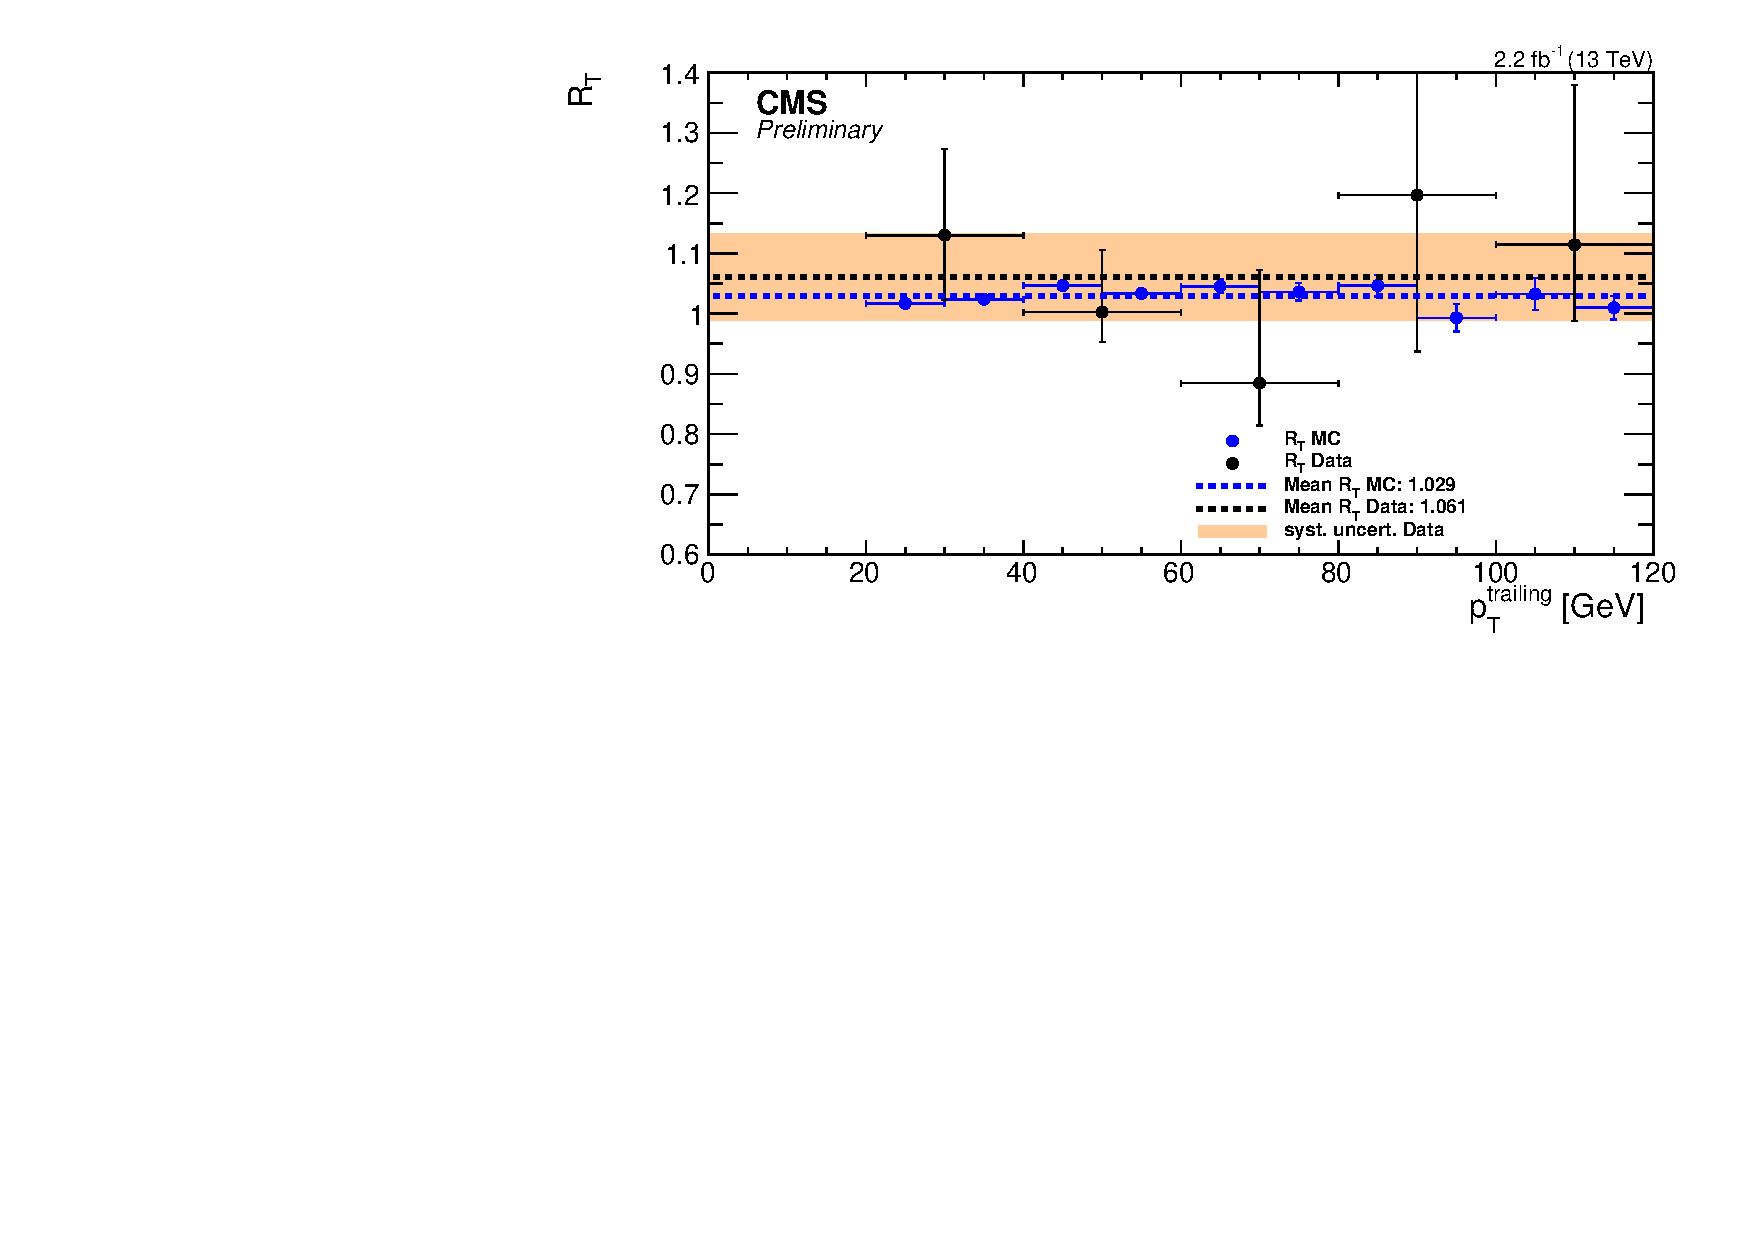
\includegraphics[width=0.30\textwidth]{bkgd/figs/Triggereff_SFvsOF_Syst_PFHT_HighHTExclusiveForward_Run2015_25ns_TrailingPt_None_NonIso_MC.pdf} \\
      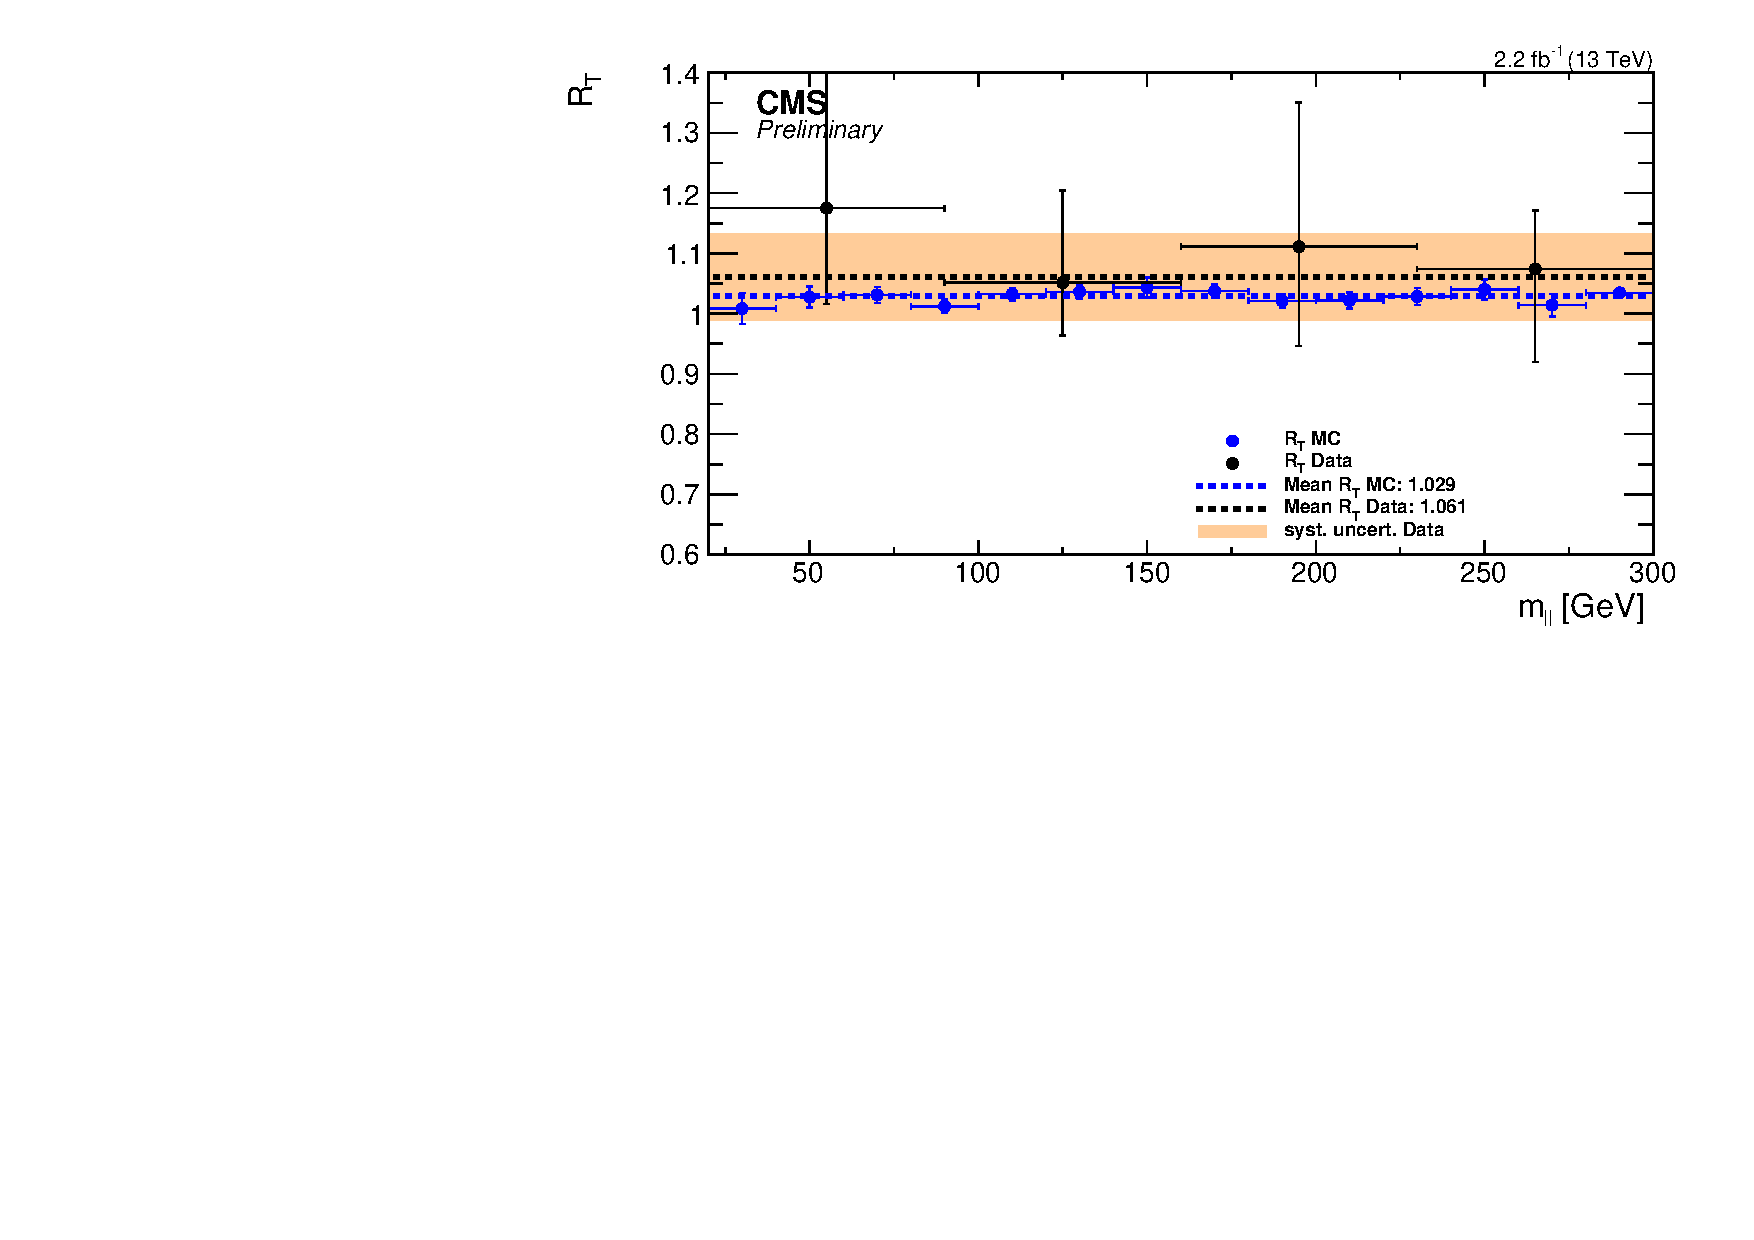
\includegraphics[width=0.30\textwidth]{bkgd/figs/Triggereff_SFvsOF_Syst_PFHT_HighHTExclusiveForward_Run2015_25ns_Mll_None_NonIso_MC.pdf} &
      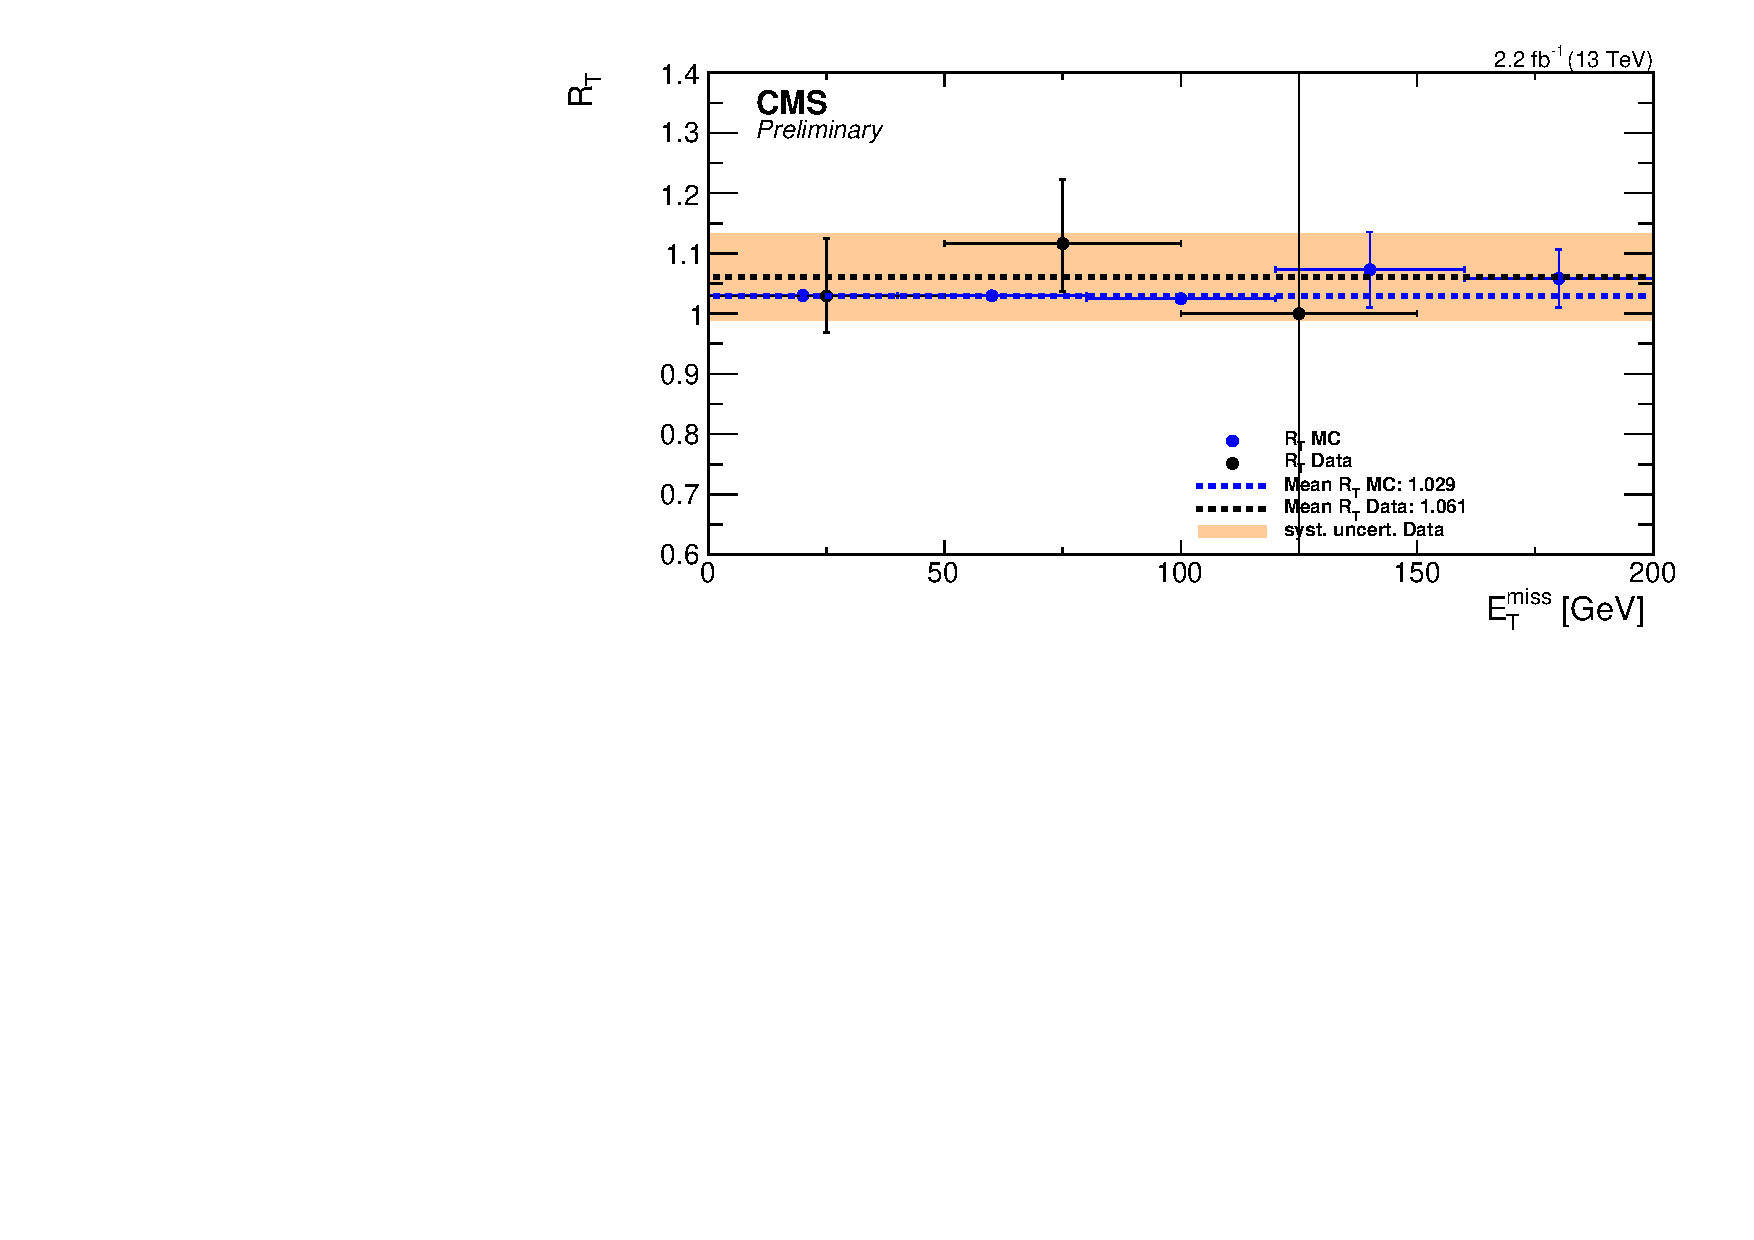
\includegraphics[width=0.30\textwidth]{bkgd/figs/Triggereff_SFvsOF_Syst_PFHT_HighHTExclusiveForward_Run2015_25ns_MET_None_NonIso_MC.pdf} &
      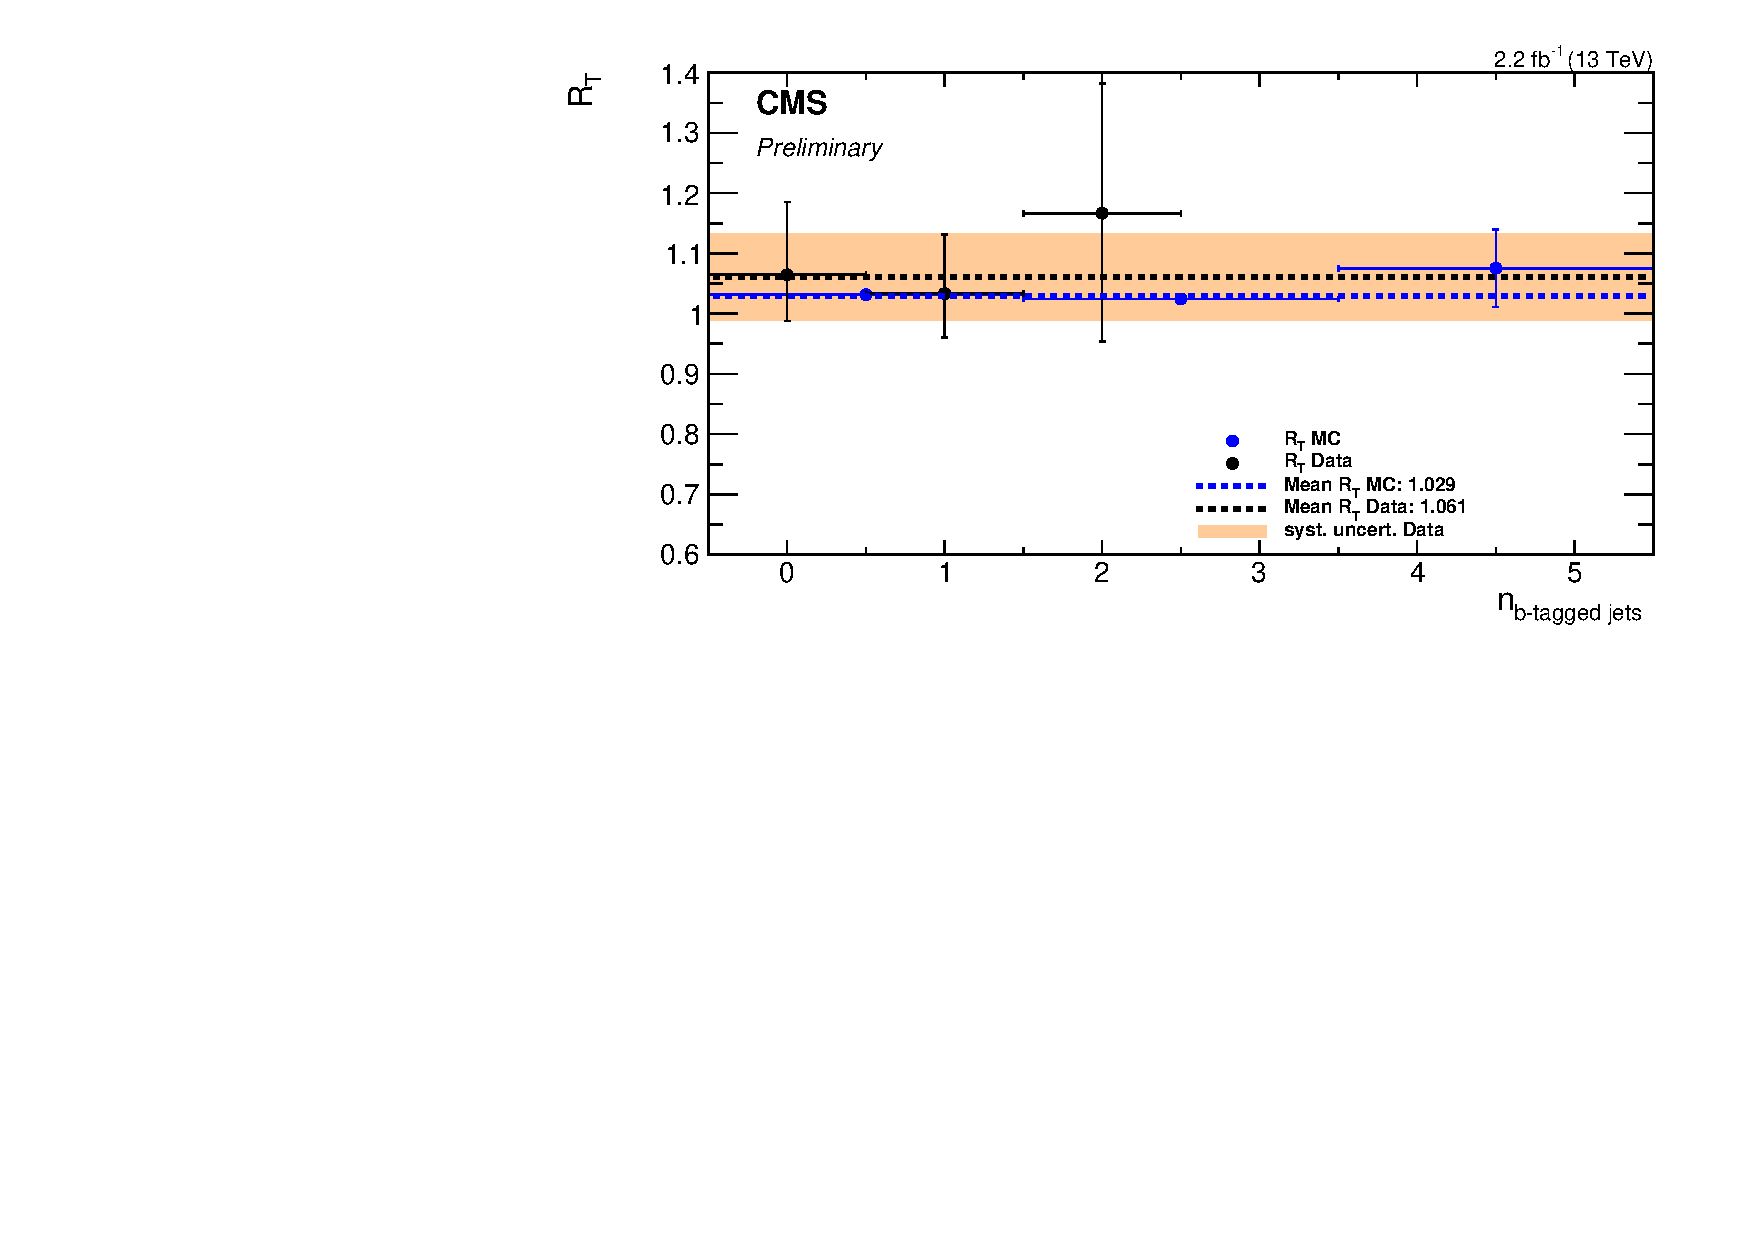
\includegraphics[width=0.30\textwidth]{bkgd/figs/Triggereff_SFvsOF_Syst_PFHT_HighHTExclusiveForward_Run2015_25ns_NBJets_None_NonIso_MC.pdf}  \\
    \end{tabular}
    \caption{
      \label{fig:EffDependencyEndcap}
      \rt\ dependency for forward leptons shown as a function of \nj, \nvtx, lepton \pt, \mll, \MET, and $N_{b-tags}$.
      The assigned 6.4\% systematic uncertainty on \rt is indicated by the orange band.
    }
  \end{center}
\end{figure}

\subsection{Results of factorizaton method}

The result of the factorization method is summarized in table~\ref{tab:factorization}.
The value and statistical uncertainty of \rsfof are both driven by \rt.
Good agreement between data and MC is observed within the uncertainties. 

\begin{table}[hbtp]
  \begin{center}
    \caption{
      \label{tab:factorization}
      The values for \rmue, \rt, and \rsfof\ are shown.
    }
    \begin{tabular}{l| c| c| c| c}
      & \multicolumn{2}{c}{Central} & \multicolumn{2}{c}{Forward} \\ 
      \hline
      & Data & MC & Data & MC \\ 
      \hline
      \rmue  &  1.14$\pm$0.11  &  1.13$\pm$0.11      &  1.23$\pm$0.25 &   1.26$\pm$0.25    \\
      $R_{T}$ &  1.00$\pm$0.07  &  1.03$\pm$0.07      &  1.06$\pm$0.09 &   1.03$\pm$0.07    \\
      \hline
      \hline
      \Rsfof &  1.01$\pm$0.07  &  1.04$\pm$0.07      &  1.08$\pm$0.1  &   1.06$\pm$0.09    \\
      \Reeof &  0.44$\pm$0.12  &  0.45$\pm$0.12      &  0.43$\pm$0.26 &   0.41$\pm$0.26    \\
      \Rmmof &  0.57$\pm$0.12  &  0.58$\pm$0.12      &  0.65$\pm$0.27 &   0.65$\pm$0.26    \\
    \end{tabular}
  \end{center}
\end{table}

\subsection{Combination of the Methods}
The results of the two methods to determine \rsfof are shown in table~\ref{tab:combinedRSFOF}.
The value for \rsfof\ in the central and forward regions is calculated using a weighted average of the two independent measurements.
This assumes that the uncertainties are sufficiently gaussian,
which is justified as they are mostly statistical in nature.
The resulting values in data are \rsfof = $1.04\pm0.05$ for central and \rsfof = $1.10\pm0.07$ for forward lepton pairs.
This results in an systematic uncertainty of 5\% and 7\% on the dominant background of the analysis in most bins.
The final value uses the weighted average of \rsfof\ from the central and forward regions,
and is calculated to be \rsfof $ = 1.05 \pm 0.04$.

\begin{table}[hbtp]
  \begin{center}
    \caption{
      \label{tab:combinedRSFOF}
      The results of the factorization method, and from direct measurement of \rsfof\ are shown.
      The values from these two methods are combined using a weighted average to get the value for \rsfof
      in the central and forward regions separately.
      These values are then combined to get the final value of \rsfof $ = 1.05 \pm 0.04$.
    }
    \begin{tabular}{l| c c| c c }
      & \multicolumn{4}{c}{\Rsfof}  \\ 
      & \multicolumn{2}{c}{Central} & \multicolumn{2}{c}{Forward} \\    
      \hline
      & Data              & MC               & Data             & MC \\ 
      \hline
      Factorization method &  1.01$\pm$0.07 & 1.04$\pm$0.07 & 1.08$\pm$0.10 & 1.06$\pm$0.09 \\
      Direct measurement   &  1.06$\pm$0.06 & 1.05$\pm$0.01 & 1.11$\pm$0.14 & 1.08$\pm$0.02 \\
      weighted avarage     &  1.04$\pm$0.05 & 1.05$\pm$0.01 & 1.10$\pm$0.07 & 1.08$\pm$0.02 \\
      \hline
      & \multicolumn{4}{c}{\Reeof}  \\ 
      & \multicolumn{2}{c}{Central} & \multicolumn{2}{c}{Forward} \\     
      \hline
      & Data & MC & Data & MC \\ 
      \hline
      Factorization method &  0.44$\pm$0.12  &  0.45$\pm$0.12      &  0.43$\pm$0.26 &   0.41$\pm$0.26    \\
      Direct measurement   &  0.43$\pm$0.04  &  0.45$\pm$0.01      &  0.46$\pm$0.11 &   0.44$\pm$0.01    \\
      weighted avarage     &  0.43$\pm$0.03  &  0.45$\pm$0.01      &  0.46$\pm$0.05 &   0.44$\pm$0.01    \\
      \hline
      & \multicolumn{4}{c}{\Rmmof}  \\ 
      & \multicolumn{2}{c}{Central} & \multicolumn{2}{c}{Forward} \\     
      \hline
      & Data & MC & Data & MC \\ 
      \hline
      Factorization method &  0.57$\pm$0.12  &  0.58$\pm$0.12      &  0.65$\pm$0.27 &   0.65$\pm$0.26    \\
      Direct measurement   &  0.63$\pm$0.05  &  0.60$\pm$0.01      &  0.65$\pm$0.12 &   0.64$\pm$0.02    \\
      weighted avarage     &  0.63$\pm$0.04  &  0.60$\pm$0.01      &  0.65$\pm$0.06 &   0.64$\pm$0.02    \\
      \hline
    \end{tabular}
  \end{center}
\end{table}

\clearpage

\subsection{MC closure test of the FS background prediction}
\label{ssec:closureFS}
In order to validate the FS background prediction method,
a closure test is performed in MC in the following way.
\rsfof, \rmue, and \rt\ are calculated using MC simulation
and subsequently used to predict the SF spectrum in \mll\ from the OF control sample.
The closure results are shown in figure~\ref{fig:closureFS}
where the blue histogram shows the predicted SF spectrum obtained using the OF sample,
and the black points show the same-flavor observation in MC.
Good closure is seen in both central and forward regions,
and the shape is seen to agree as well.
It is also clear from the same figure that this method
works regardless of the number of required b-tagged jets.

\begin{figure}[htb]
  \begin{center}
    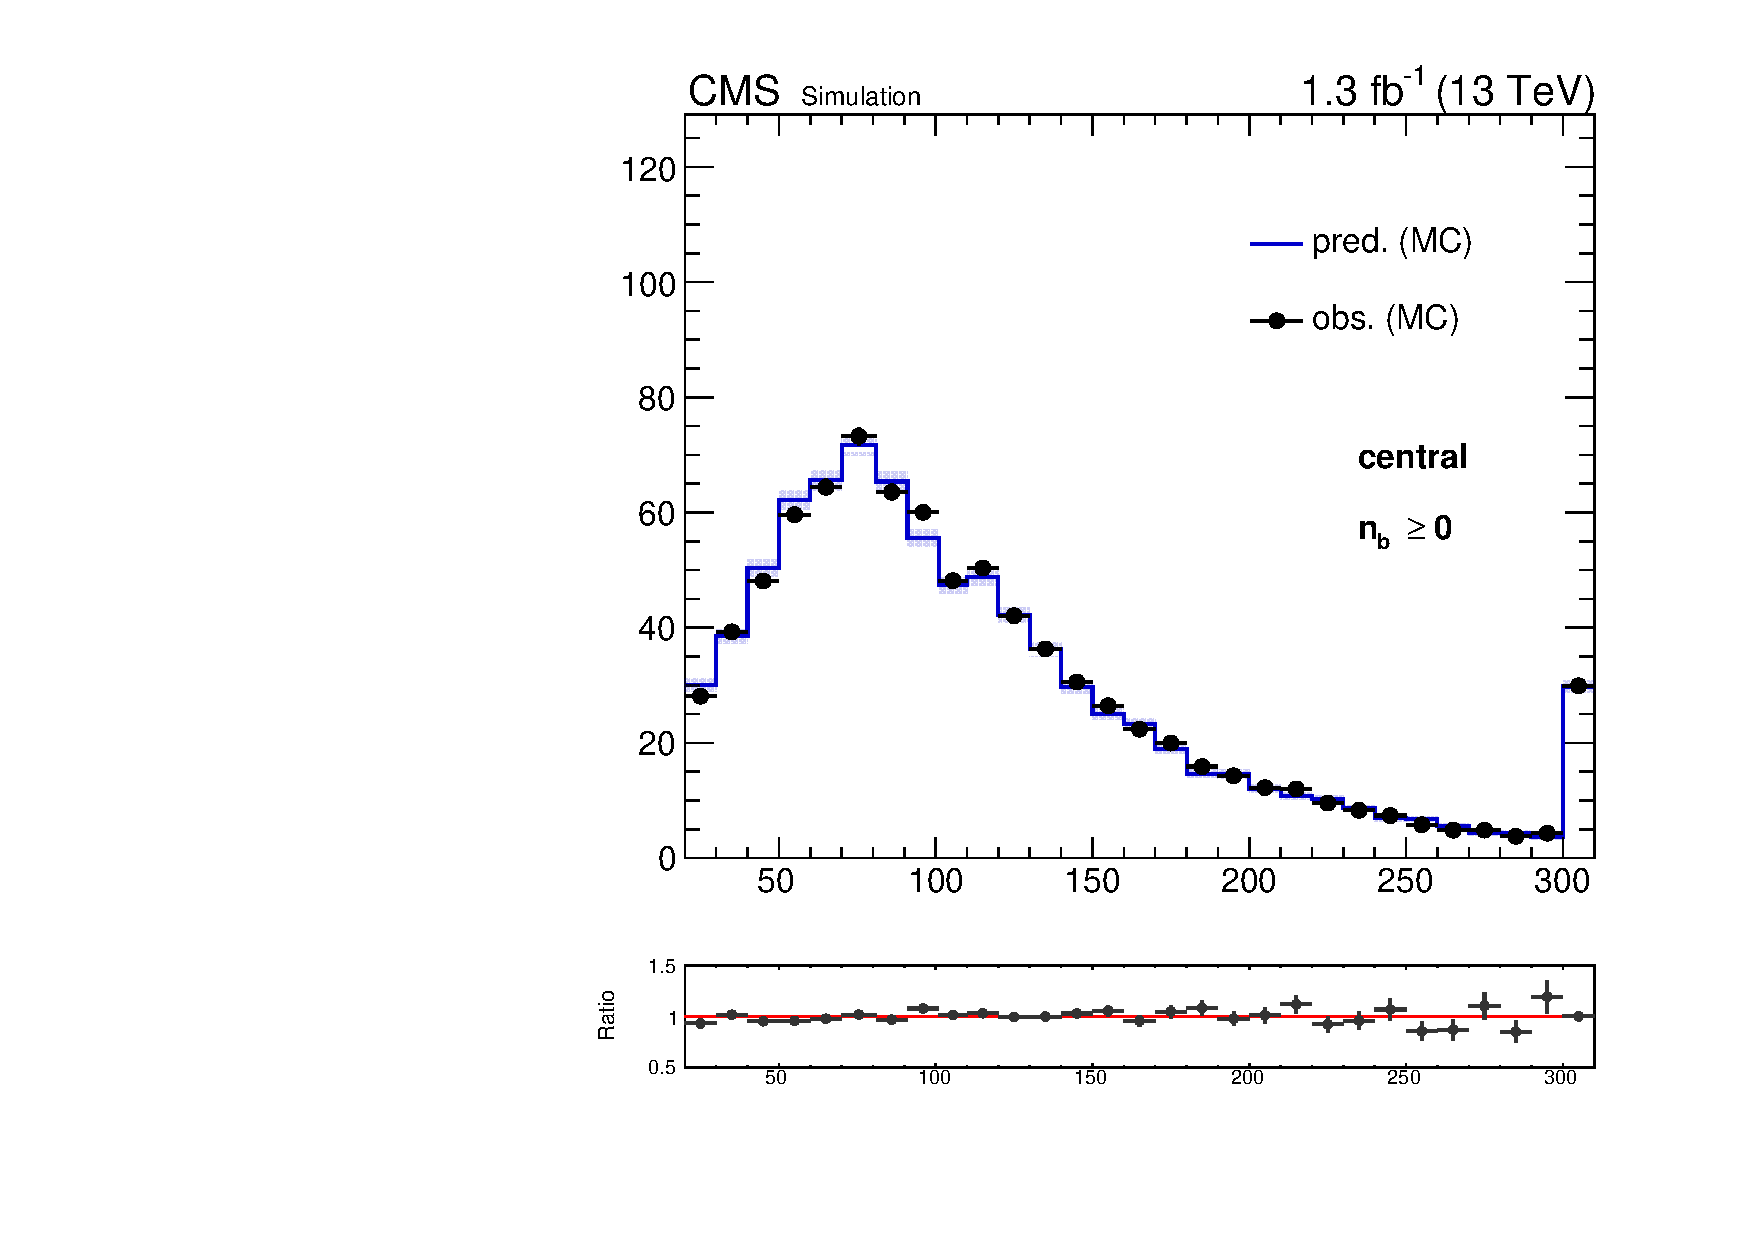
\includegraphics[scale=0.25]{bkgd/figs/plot_results_mll_MCClosure_central_onlyTT_nbInc.pdf}
    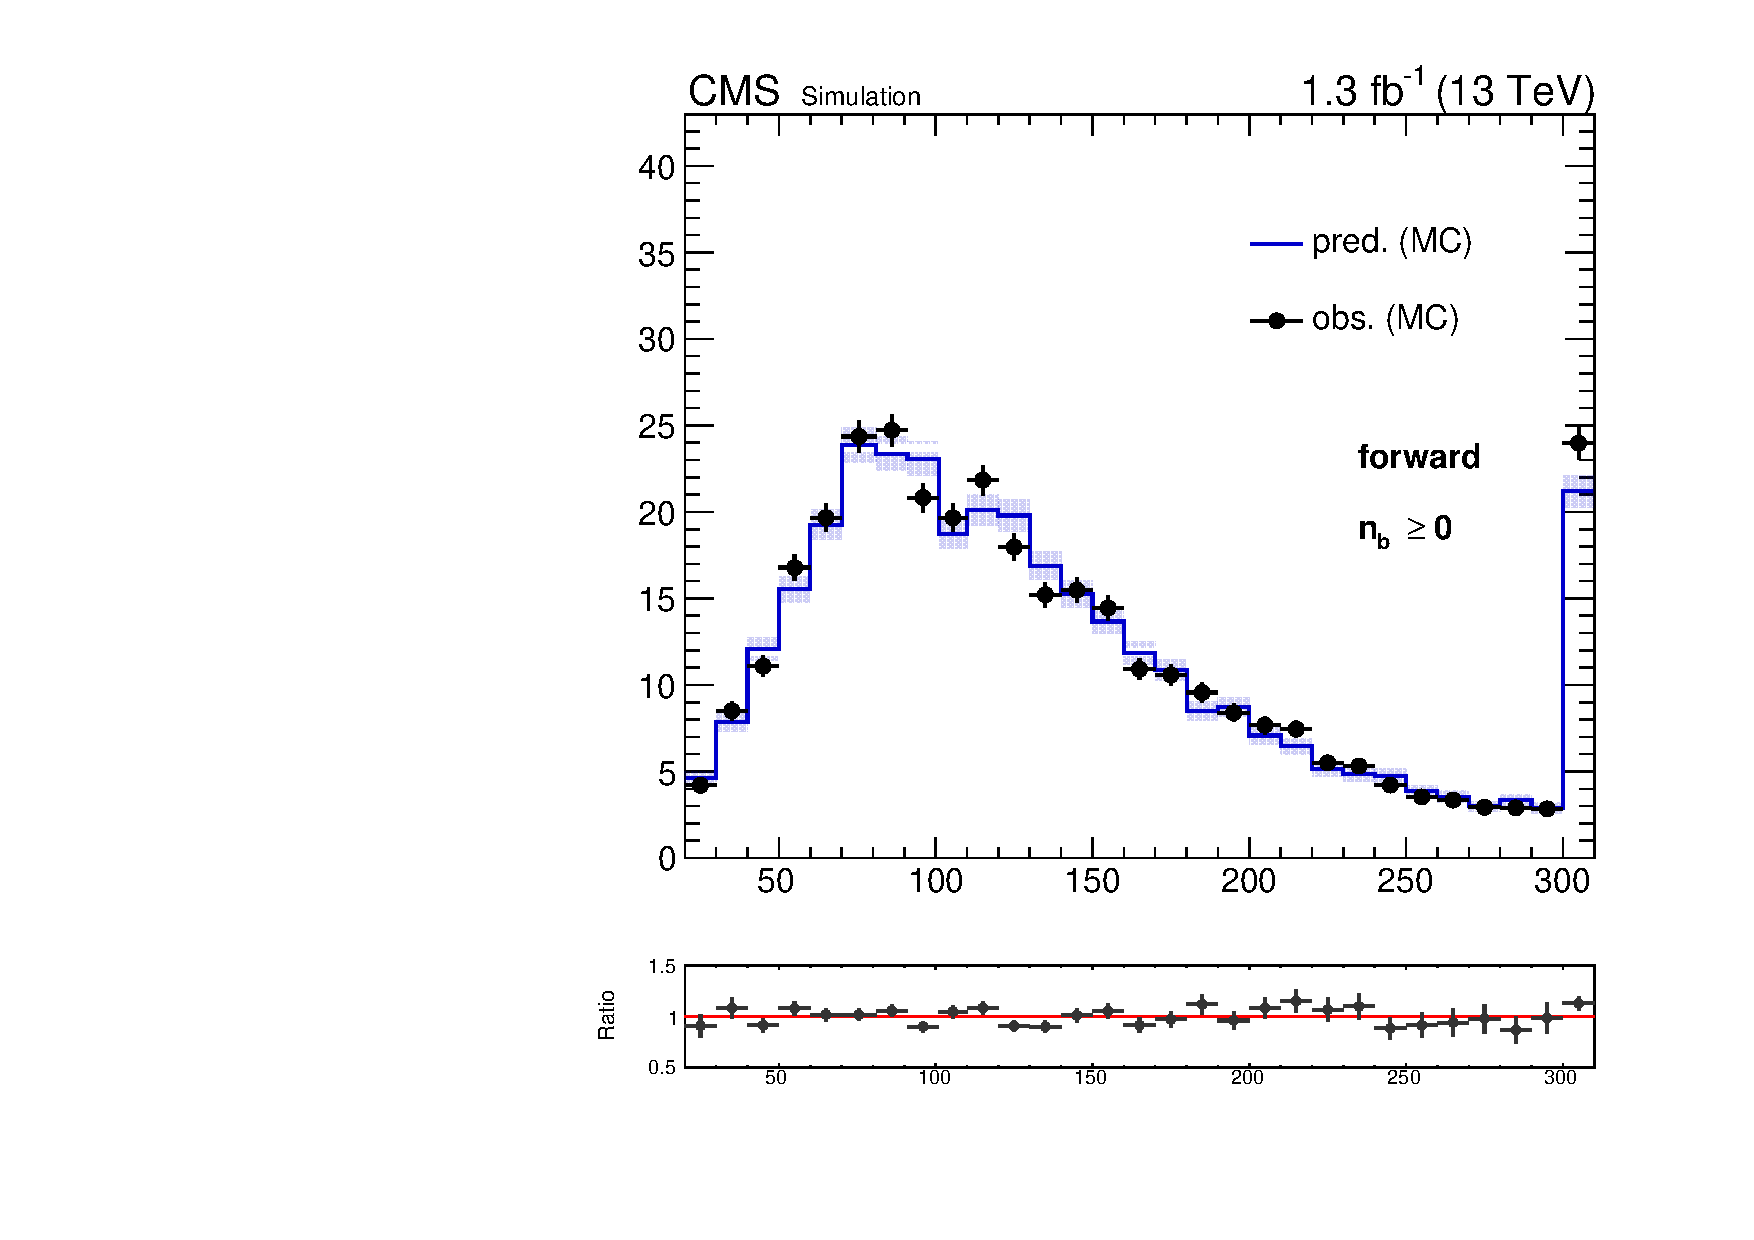
\includegraphics[scale=0.25]{bkgd/figs/plot_results_mll_MCClosure_forward_onlyTT_nbInc.pdf}\\
    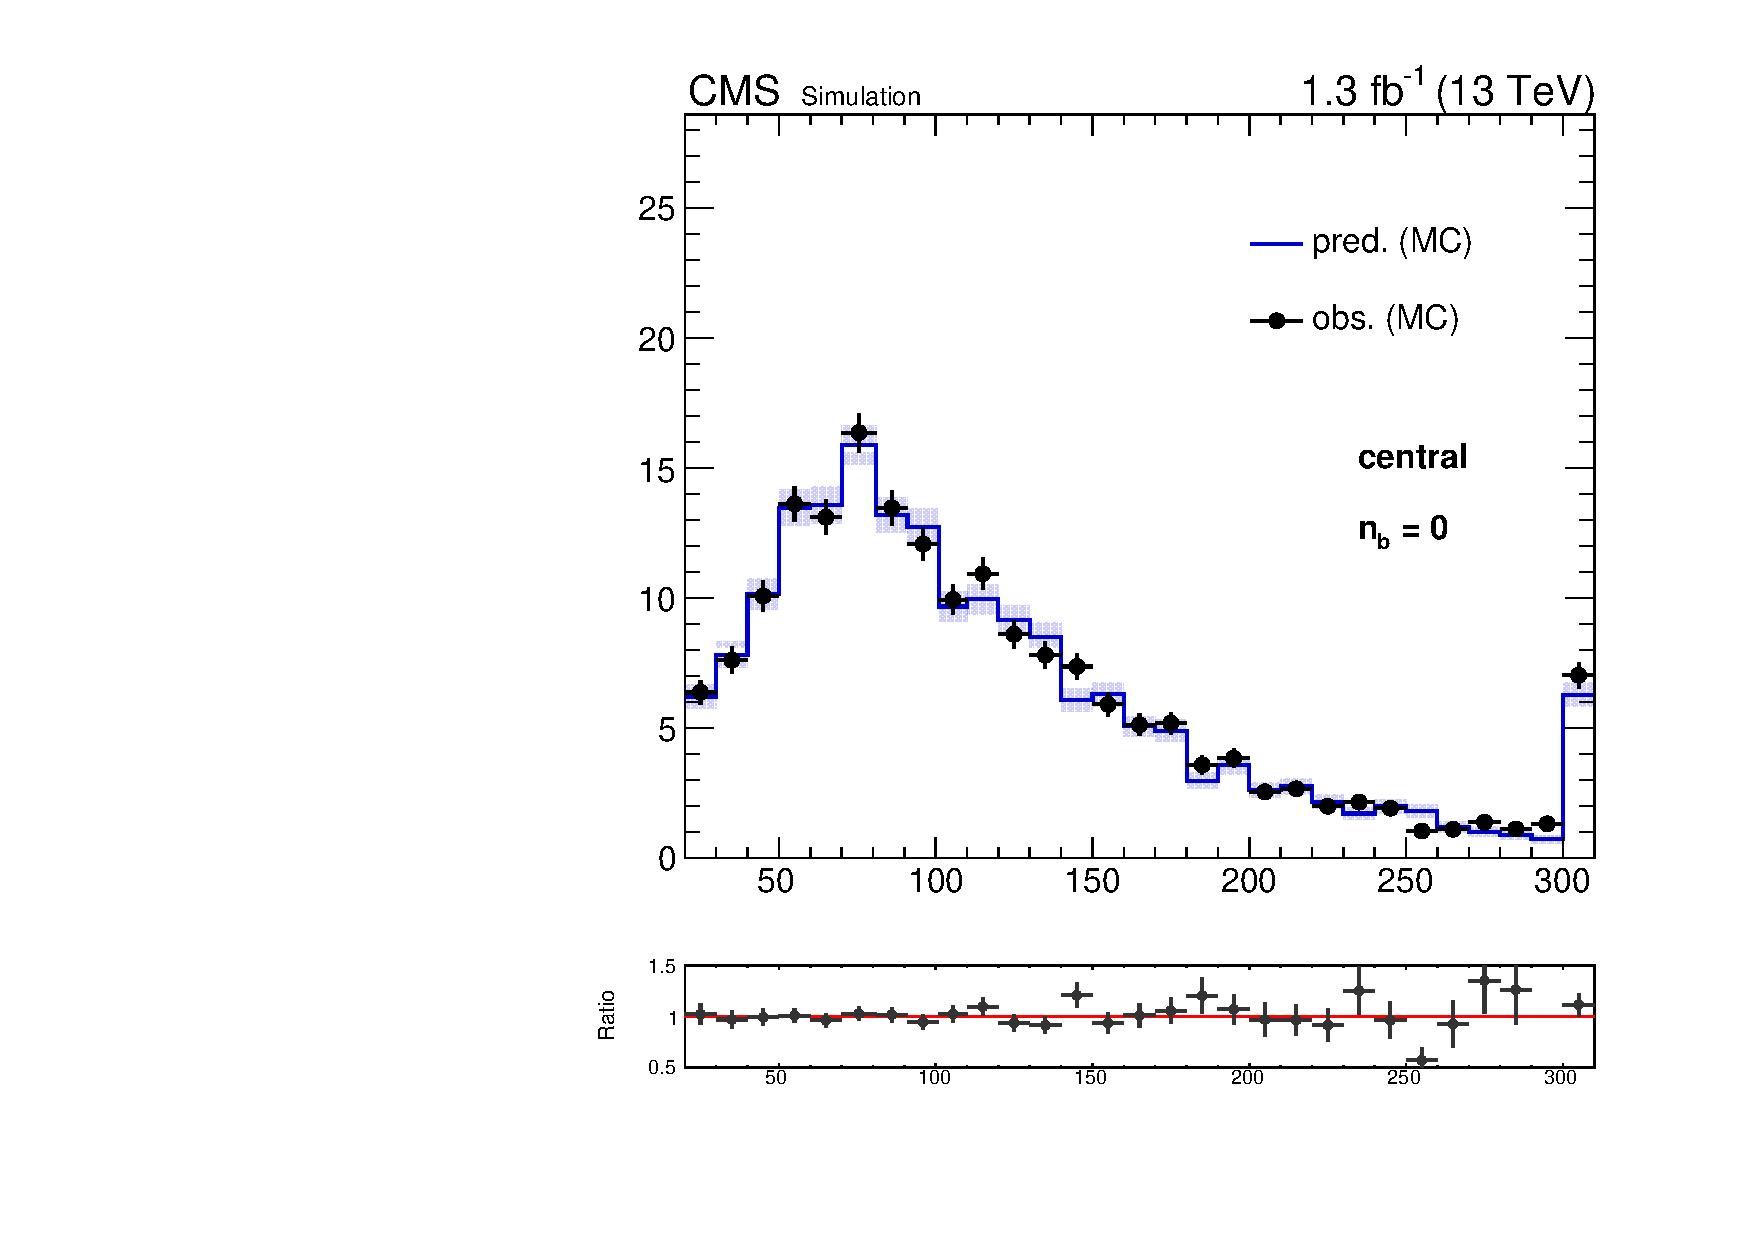
\includegraphics[scale=0.25]{bkgd/figs/plot_results_mll_MCClosure_central_onlyTT_nb0.pdf}
    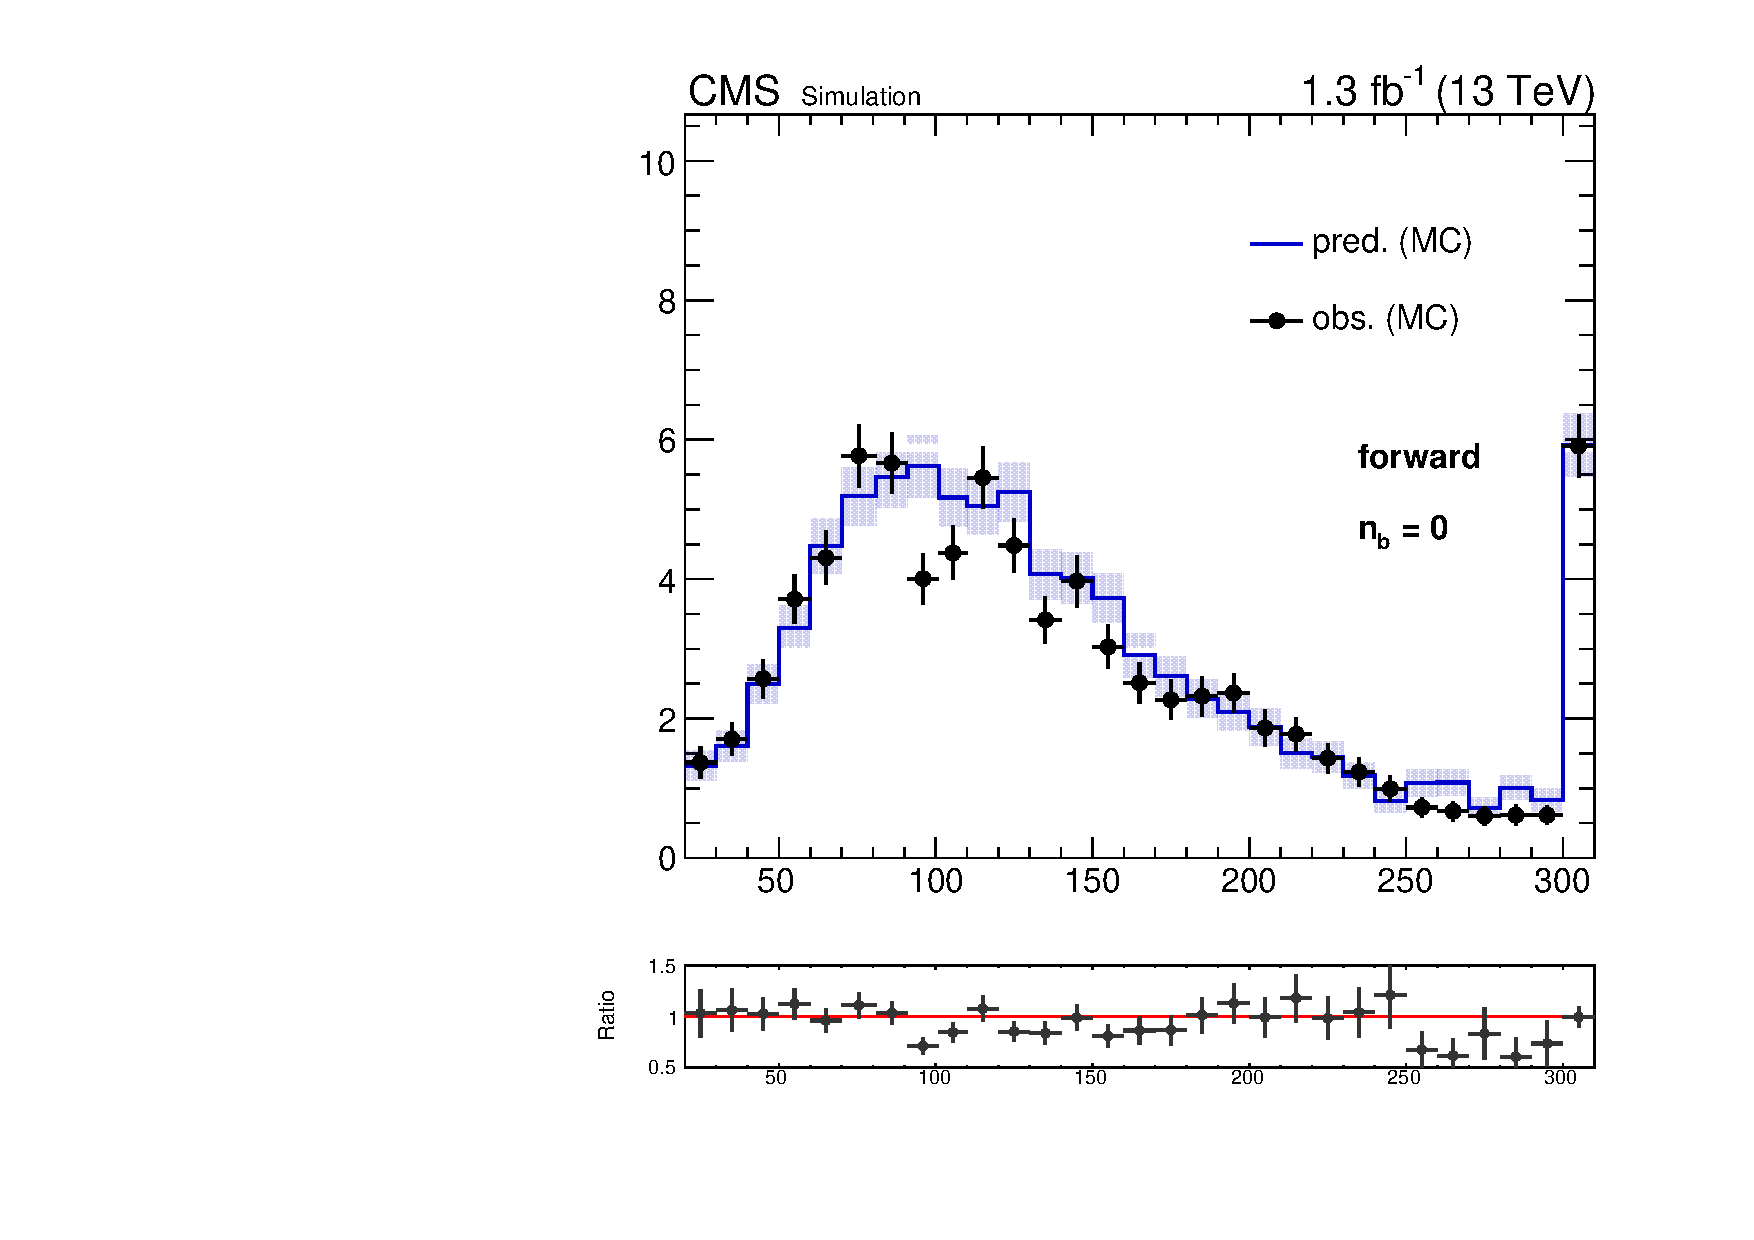
\includegraphics[scale=0.25]{bkgd/figs/plot_results_mll_MCClosure_forward_onlyTT_nb0.pdf} \\
    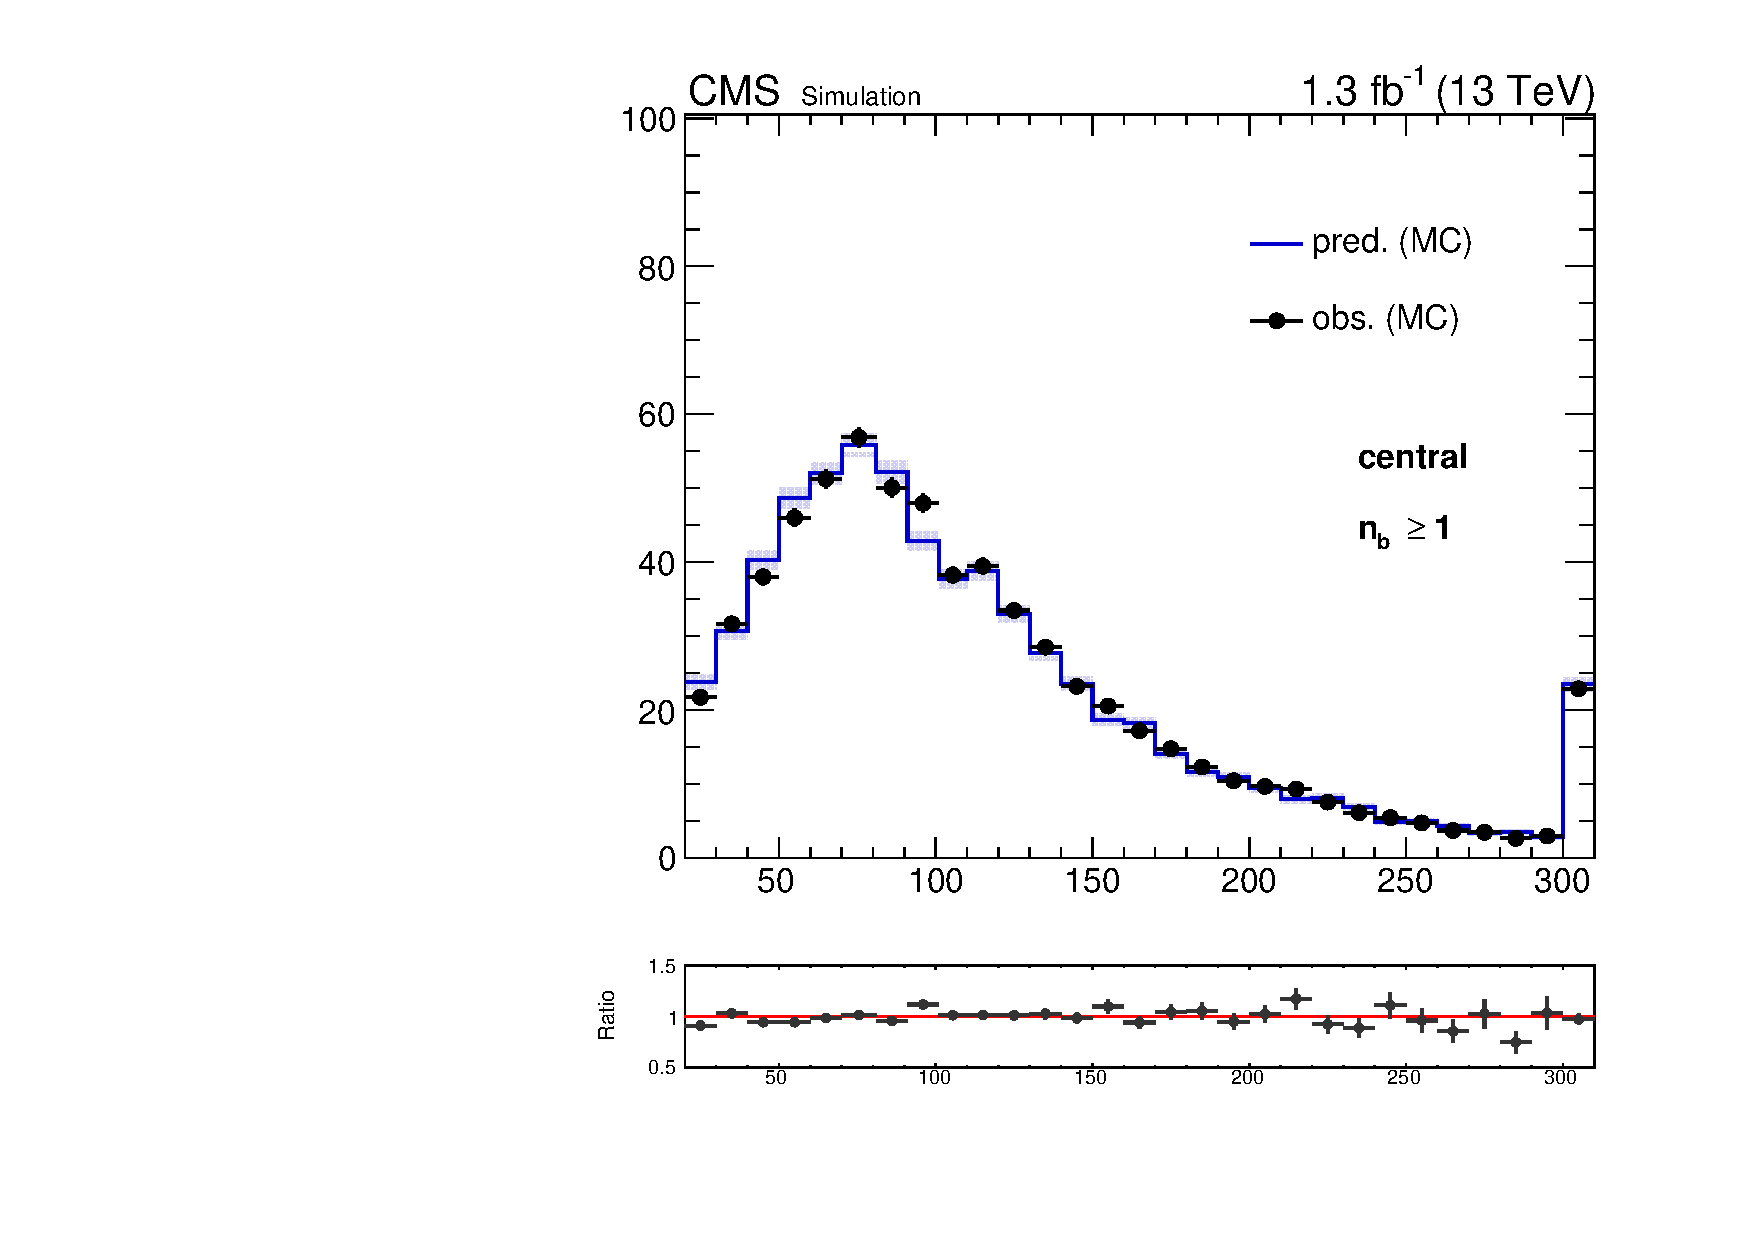
\includegraphics[scale=0.25]{bkgd/figs/plot_results_mll_MCClosure_central_onlyTT_nb1.pdf}
    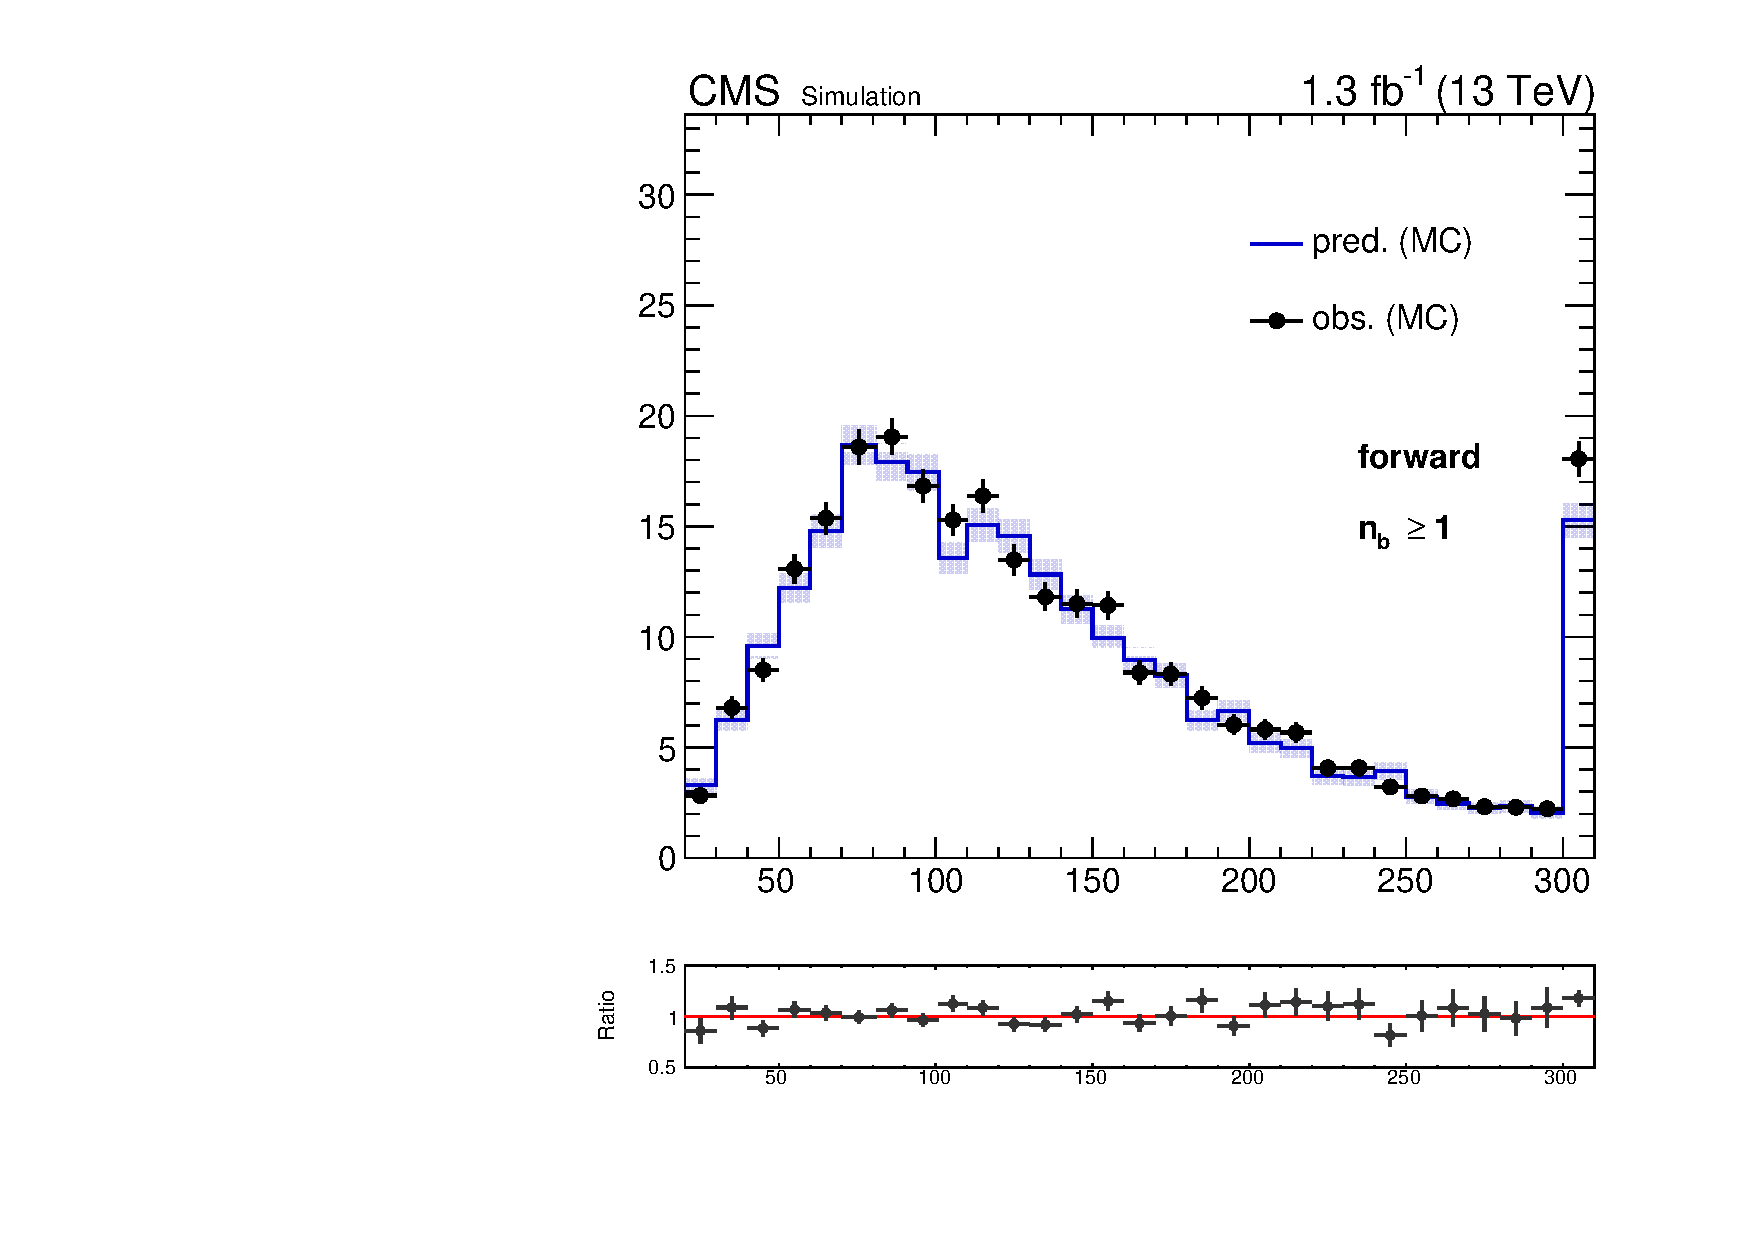
\includegraphics[scale=0.25]{bkgd/figs/plot_results_mll_MCClosure_forward_onlyTT_nb1.pdf}\\
    \caption{
      MC closure test for central (left) and forward (right) in the \mll variable.
      The blue histogram shows the MC prediction from the OF sample by multiplying
      with \rsfof whereas the black markers correspond to the observation in the SF sample.
      This exercise is done on \ttbar MC only, and is shown for all number of b-tagged jet bins.
      The top row shows the closure test for inclusive,
      the middle row 0 b-tagged jets and the bottom row $\geq$ 1 jets.
    }
    \label{fig:closureFS}
  \end{center}
\end{figure}

Results of the closure test are shown in table~\ref{tab:MCClosure}.
The observed values of SF events are compared to the number of
OF events scaled by the \rsfof value obtained using MC simulation for different processes.
Only the statistical uncertainty on the event yield is shown.
The dominant background is from \ttbar\ as expected and observed to be well-predicted using the FS method.
Good closure is also seen in sub-dominant backgrounds such as single top quark production and \DYjets $\rightarrow \tau\tau$.
Non FS backgrounds, such as \DYjets $\rightarrow ee,~\mu\mu$ or rare processes involving \Z boson production,
are not predicted well, as expected.

\begin{table}[hbtp]
  \begin{center}
    \caption{
      Event yields in the signal region in simulation for both SF and OF lepton pairs.
      The OF yield is multiplied with \Rsfof.
      The quoted uncertainties are those of the MC counts in the signal region only.
    }
    \label{tab:MCClosure}
    \begin{tabular}{l| ccc | ccc }
      & \multicolumn{3}{c|}{Central} & \multicolumn{3}{c}{Forward} \\ 
      \hline
	  &  SF       & OF        &  SF-OF   & SF        &  OF       & SF-OF    \\ 
      \hline
      \ttbar                & 863$\pm$5 & 860$\pm$5 &  2$\pm$7 & 362$\pm$3 & 356$\pm$3 &  5$\pm$4 \\
      \DYjets (ee,$\mu\mu$) &  19$\pm$6 &   0$\pm$0 & 18$\pm$6 &  14$\pm$4 &   0$\pm$0 & 14$\pm$4 \\
      \DYjets $(\tau \tau)$ &  11$\pm$6 &  20$\pm$5 & -8$\pm$8 &   6$\pm$2 &   4$\pm$3 &  2$\pm$4 \\
      Single t              &  53$\pm$1 &  52$\pm$1 &  0$\pm$2 &  21$\pm$1 &  21$\pm$1 &  0$\pm$1 \\
      WW, \Z{}\Z, W\Z       &  22$\pm$0 &  15$\pm$0 &  7$\pm$0 &  10$\pm$0 &   8$\pm$0 &  1$\pm$0 \\
      Other SM              &   9$\pm$0 &   5$\pm$0 &  3$\pm$0 &   4$\pm$0 &   3$\pm$0 &  0$\pm$0 \\
      \hline
      Total MC simulation & 980$\pm$10 & 955$\pm$7 & 24$\pm$13 & 419$\pm$6 & 394$\pm$4 & 24$\pm$8 \\
    \end{tabular}
  \end{center}
\end{table}


\clearpage

\section{Estimating WZ, ZZ and other rare SM backgrounds with Simulation}
\label{sec:bkg_rareSMBG}

In this section, we consider the systematic uncertainty in the WZ and ZZ background predictions both of which are taken from MC.
We do this by defining two control regions where we can study these backgrounds.
To study the WZ sample, we require there be exactly 3 leptons in the event with \pt~$>$20 \gev.
We then require 2 of the 3 leptons makes an OSSF pair which has \mll~81 to 101 GeV.
To study the ZZ sample, we require there be exactly 4 leptons in the event with \pt~$>$20 \gev.
We then require 2 of the 4 leptons makes an OSSF pair which has \mll~81 to 101 GeV.

The results of this study is shown in sections~\ref{sec:bkg_WZ}~and~\ref{sec:bkg_ZZ}.
Because of the limited amount of data, we only show the \MET\ and \nj\ distributions.

\subsubsection{3 lepton Control Region}
\label{sec:bkg_WZ}

We define a control region where we can compare the WZ MC to data by selecting events with exactly 3 leptons.
The full requirements are listed below:

\begin{itemize}
\item exactly 3 leptons with \pt\ $>$ 20 \gev
\item at least 2 leptons form an OSSF pair with \mll:81-101 \gev
\item veto events with $\geq$ 1 b-tagged jet
\item \MET\ $>$ 50 \gev 
\end{itemize}

From the limited statistics we have in this region, we see good closure for the MC to predict data.
We assign an systematic uncertainty of 50\% to the background predictions from this MC in our signal region.

\begin{figure}[!htb]
\begin{center}
\begin{tabular}{cc}
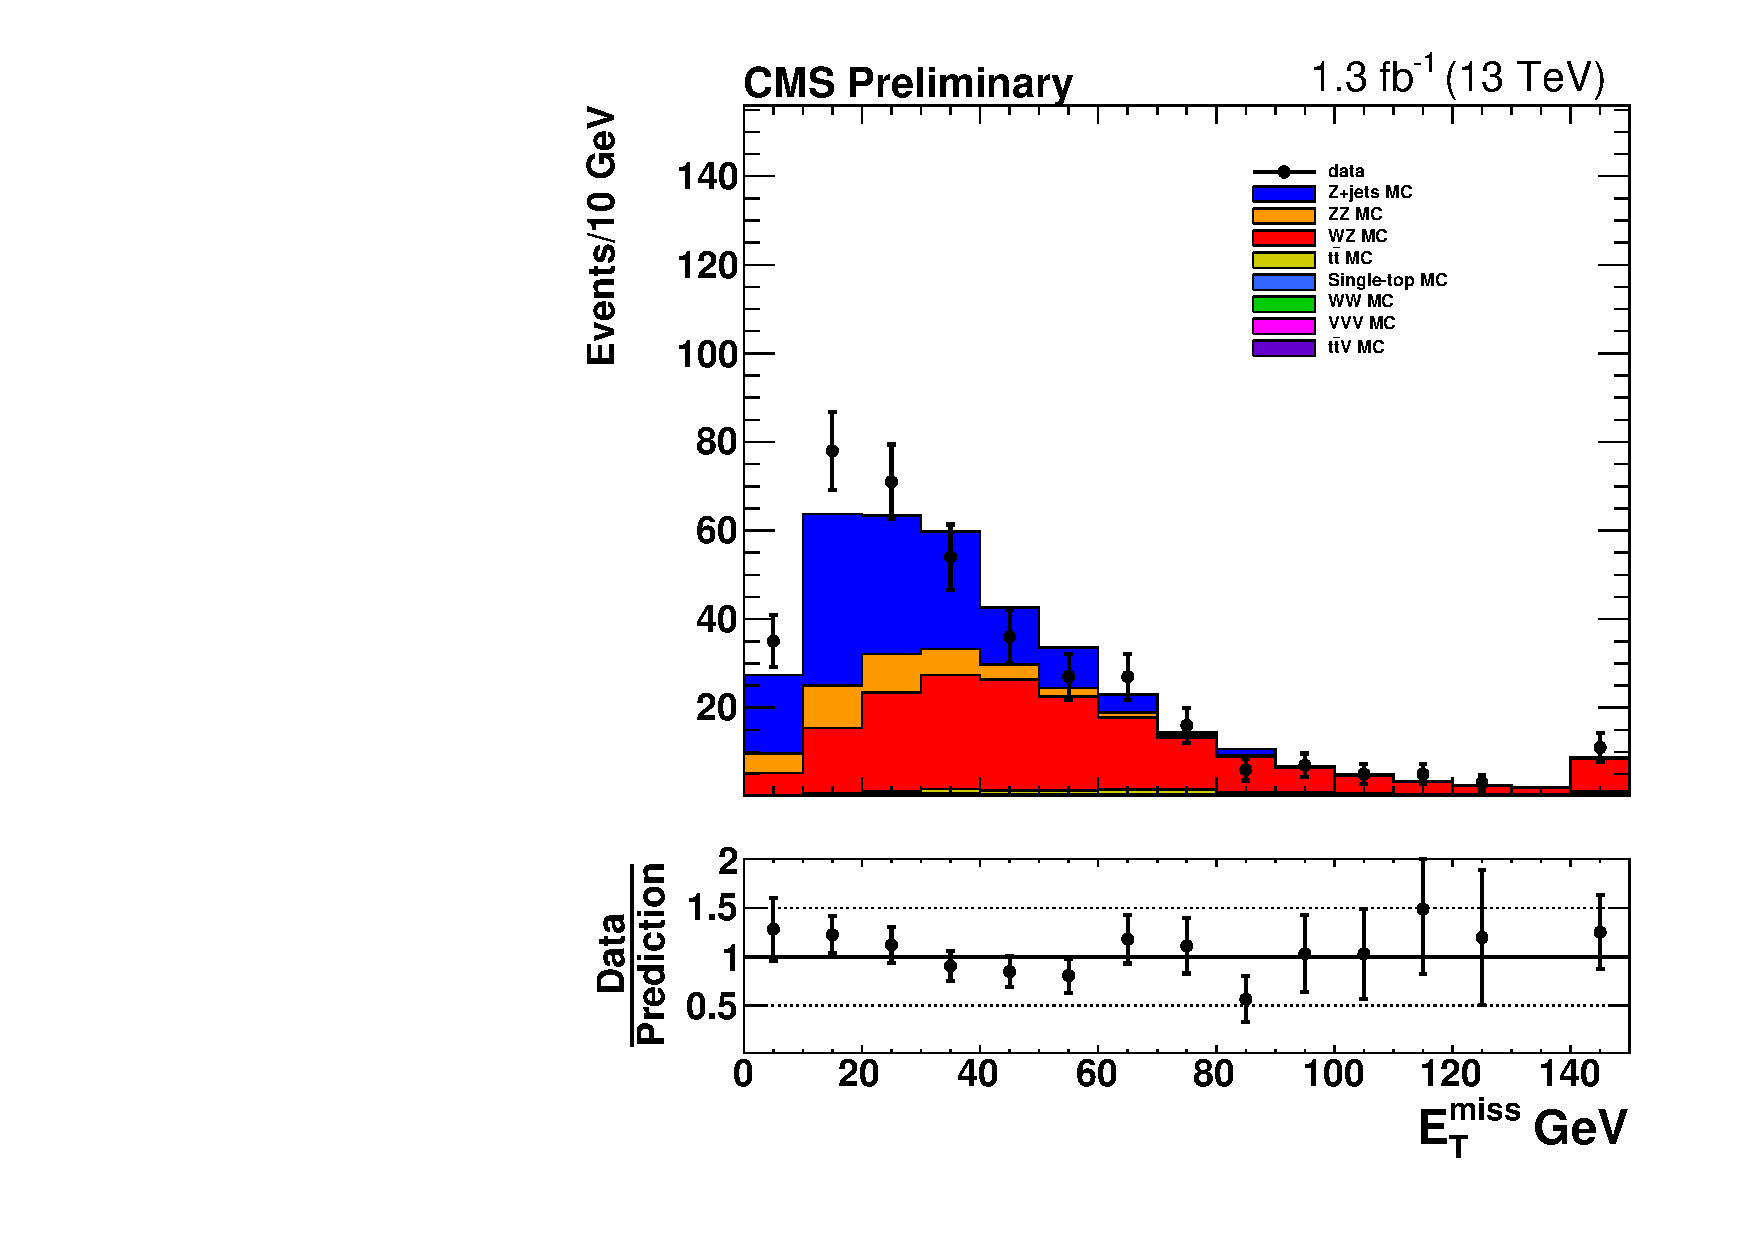
\includegraphics[width=0.4\textwidth]{bkgd/figs/h_metall_ll_signalregion_CR3lep_passtrig.pdf} &
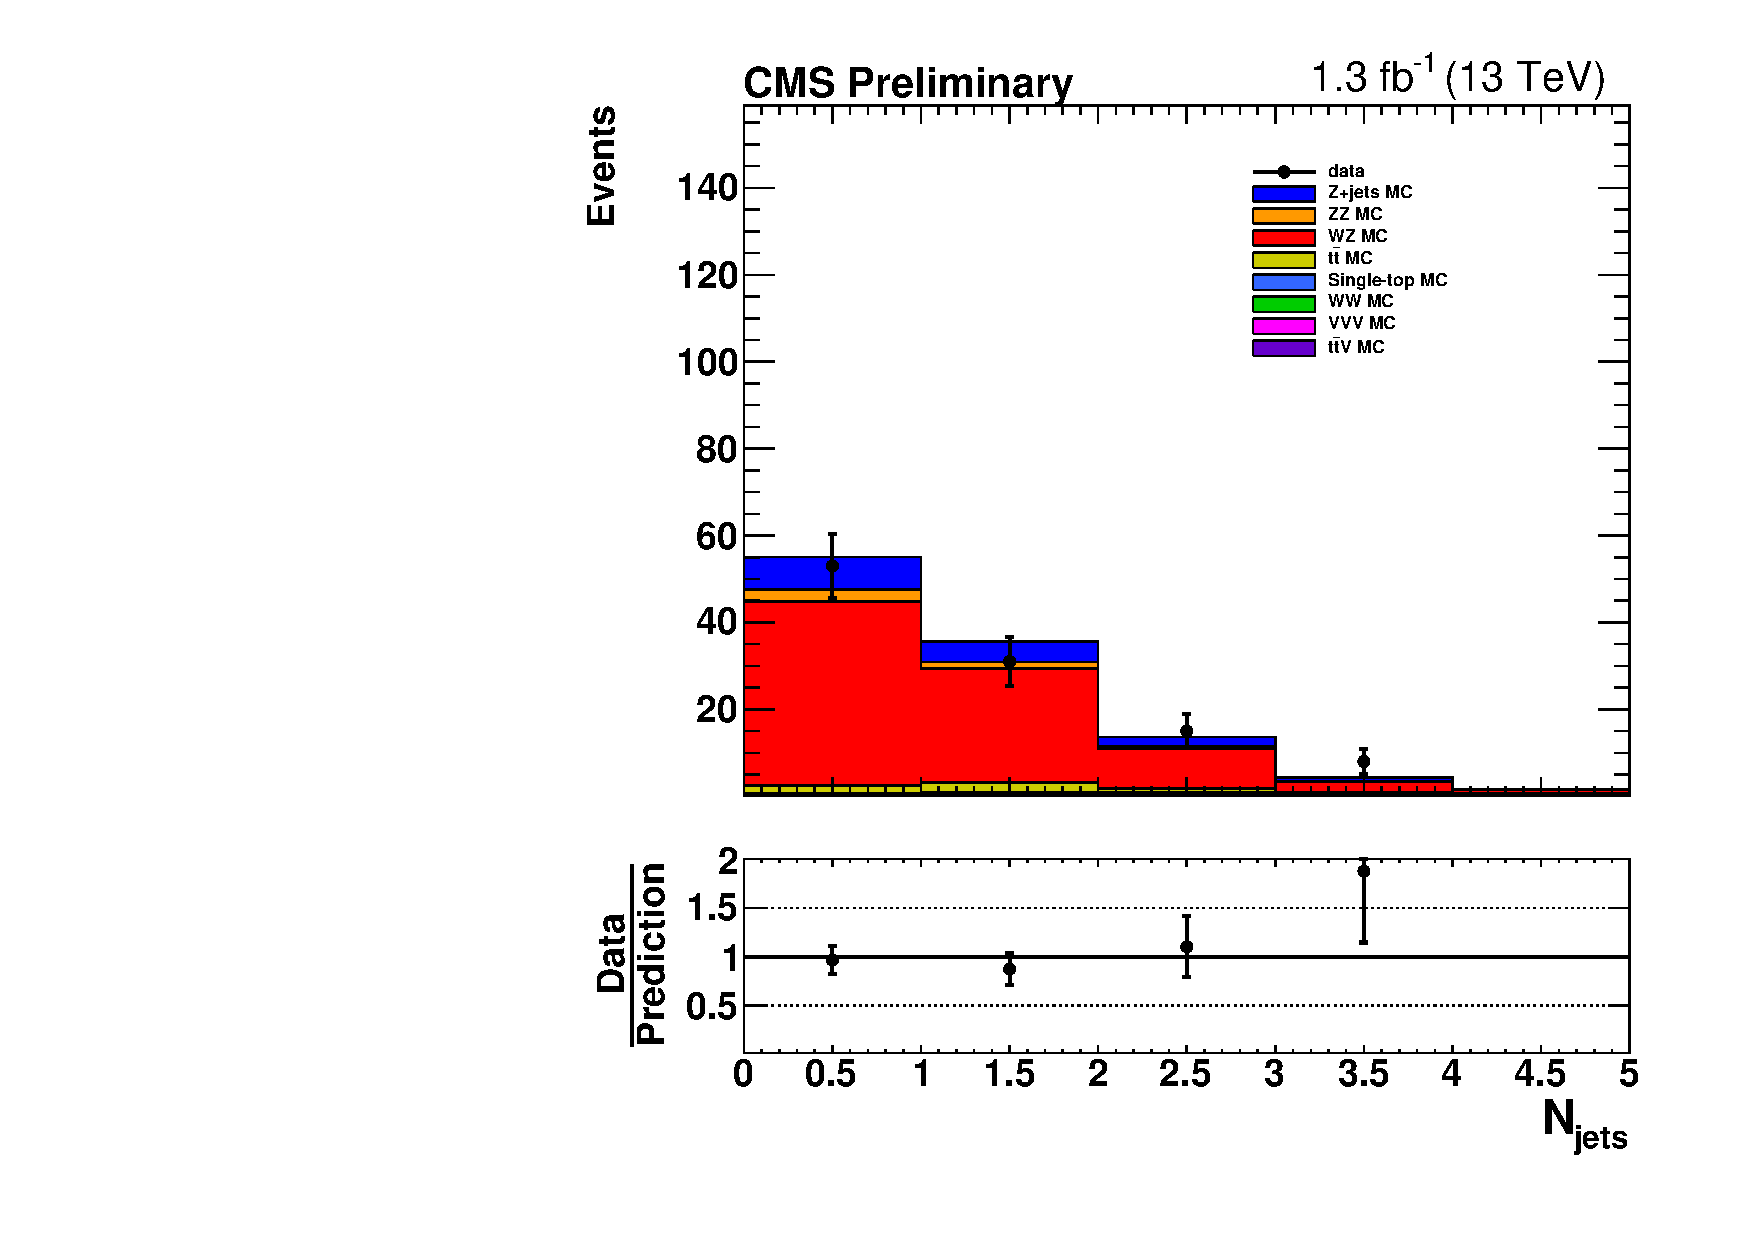
\includegraphics[width=0.4\textwidth]{bkgd/figs/h_njtm50_ll_signalregion_CR3lep_passtrig.pdf} \\
\end{tabular}
\caption{The \MET\ and \nj\ distributions are shown for data vs. MC in the 3-lepton control region.
  We require \MET\ $>$ 50 \gev\ for the events shown in the \nj\ distribution.
See Tables~\ref{tab:met_CR3lep}~and~\ref{tab:njets_CR3lep}~for yields.
\label{fig:bkg_CR3lep}
}
\end{center}
\end{figure}



\begin{table}[htb]
  \scriptsize
  \begin{center}
    \caption{\label{tab:met_CR3lep} 
      Yields in the 3-lepton control region binned in \MET. Uncertainties for each region are statistical only. 
    }
    \begin{tabular}{l|c|c|c|c}
      \hline
      \hline
      $\mathrm{E_{T}^{miss} [GeV]}$ &0 - 50 & 50 - 100 & 100 - 150 & $\geq$ 150 \\
      \hline 
      Z+jets&  127.2 $\pm$ 13.1 &  15.0 $\pm$ 4.0 &  0.1 $\pm$ 0.1 &  $<$ 0.1 \\ 
      FS bkg&  2.6 $\pm$ 0.3 &  3.8 $\pm$ 0.4 &  1.2 $\pm$ 0.2 &  0.4 $\pm$ 0.1 \\ 
      WZ + ZZ bkg&  125.0 $\pm$ 0.7 &  67.5 $\pm$ 0.5 &  11.9 $\pm$ 0.2 &  6.5 $\pm$ 0.2 \\ 
      ttv SM BG&  0.8 $\pm$ 0.0 &  0.7 $\pm$ 0.0 &  0.3 $\pm$ 0.0 &  0.3 $\pm$ 0.0 \\ 
      vvv SM BG&  0.8 $\pm$ 0.1 &  1.1 $\pm$ 0.1 &  0.6 $\pm$ 0.1 &  0.3 $\pm$ 0.0 \\ 
      \hline 
      total BG&  256.4 $\pm$ 13.1 &  88.0 $\pm$ 4.1 &  14.0 $\pm$ 0.3 &  7.4 $\pm$ 0.2 \\ 
      \hline 
      Data&  274 &  83 &  15 &  9 \\ 
      \hline 
      Data/BG&  1.07 $\pm$ 0.08 &  0.94 $\pm$ 0.11 &  1.07 $\pm$ 0.28 &  1.21 $\pm$ 0.41 \\ 
      \hline
      \hline
    \end{tabular}
  \end{center}
\end{table}


\begin{table}[htb]
  \scriptsize
  \begin{center}
    \caption{\label{tab:njets_CR3lep} 
      Yields in the 3-lepton control region split by \nj. Uncertainties for each region are statistical only. 
    }
    \begin{tabular}{l|c|c|c|c|c}
      \hline
      \hline
      $\mathrm{N_{jets}}$ &0  & 1  & 2  & 3  & $\geq$ 4 \\
      \hline 
      Z+jets&  7.4 $\pm$ 2.8 &  4.7 $\pm$ 2.3 &  2.2 $\pm$ 1.7 &  0.8 $\pm$ 0.7 &  $<$ 0.1 \\ 
      FS bkg&  1.7 $\pm$ 0.2 &  2.2 $\pm$ 0.3 &  0.9 $\pm$ 0.2 &  0.3 $\pm$ 0.1 &  0.1 $\pm$ 0.1 \\ 
      WZ + ZZ bkg&  45.2 $\pm$ 0.4 &  27.8 $\pm$ 0.4 &  9.6 $\pm$ 0.2 &  2.6 $\pm$ 0.1 &  0.7 $\pm$ 0.1 \\ 
      ttv SM BG&  0.2 $\pm$ 0.0 &  0.4 $\pm$ 0.0 &  0.3 $\pm$ 0.0 &  0.2 $\pm$ 0.0 &  0.1 $\pm$ 0.0 \\ 
      vvv SM BG&  0.1 $\pm$ 0.0 &  0.4 $\pm$ 0.0 &  0.6 $\pm$ 0.1 &  0.4 $\pm$ 0.1 &  0.5 $\pm$ 0.1 \\ 
      \hline 
      total BG&  54.6 $\pm$ 2.8 &  35.5 $\pm$ 2.3 &  13.6 $\pm$ 1.7 &  4.3 $\pm$ 0.7 &  1.5 $\pm$ 0.1 \\ 
      \hline 
      Data&  53 &  31 &  15 &  8 &  0 \\ 
      \hline 
      Data/BG&  0.97 $\pm$ 0.14 &  0.87 $\pm$ 0.17 &  1.10 $\pm$ 0.31 &  1.88 $\pm$ 0.73 &  -- \\ 
      \hline
      \hline
    \end{tabular}
  \end{center}
\end{table}


\subsubsection{4 lepton Control Region}
\label{sec:bkg_ZZ}


We define a control region where we can compare the ZZ MC to data by selecting events with exactly 4 leptons.
The full requirements are listed below:

\begin{itemize}
\item exactly 4 leptons with \pt\ $>$ 20 \gev
\item at least 2 leptons form an OSSF pair with \mll:81-101 \gev
\end{itemize}

From the limited statistics we have in this region, we see reasonable closure for the MC to predict data.
We assign an systematic uncertainty of 50\% to the background predictions from this MC in our signal region.


\begin{figure}[!htb]
\begin{center}
\begin{tabular}{cc}
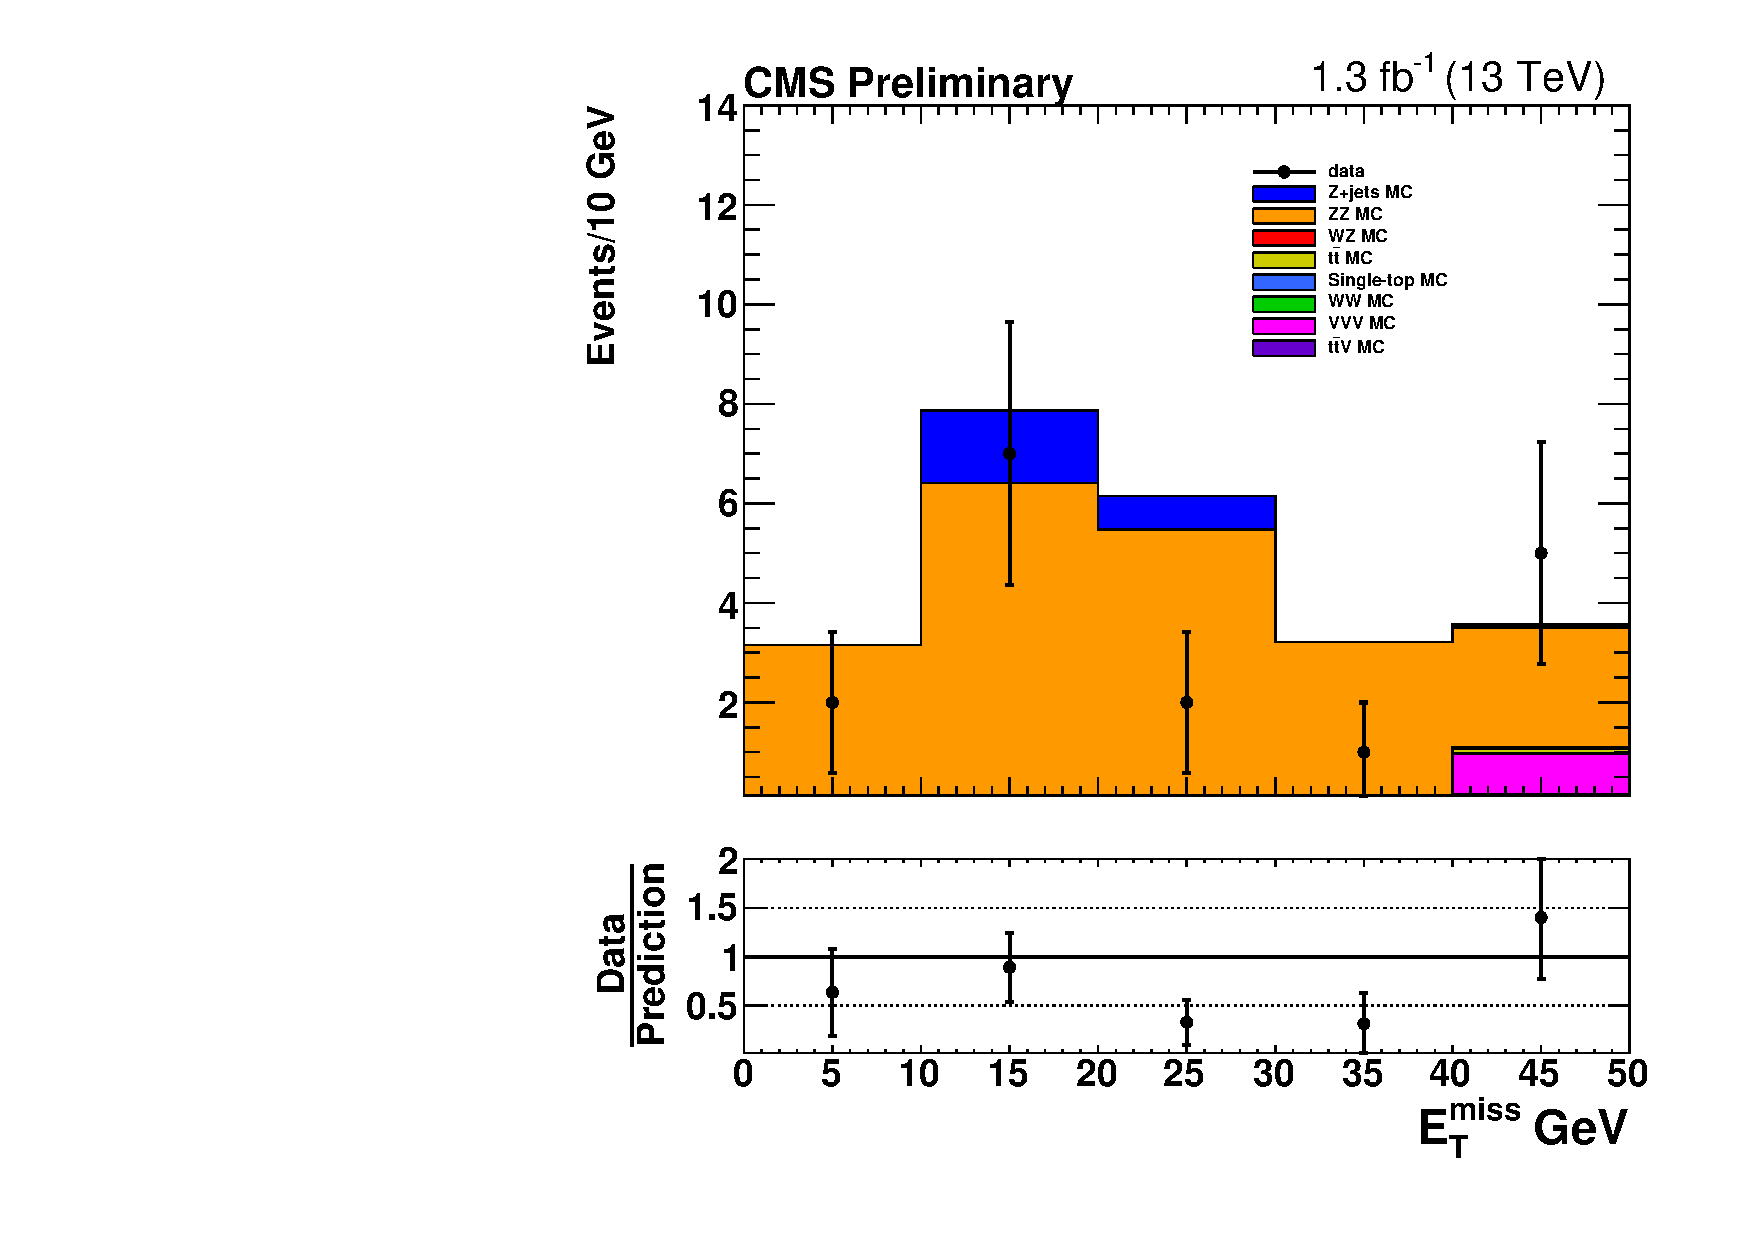
\includegraphics[width=0.4\textwidth]{bkgd/figs/h_metall_ll_signalregion_CR4lep_passtrig.pdf} &
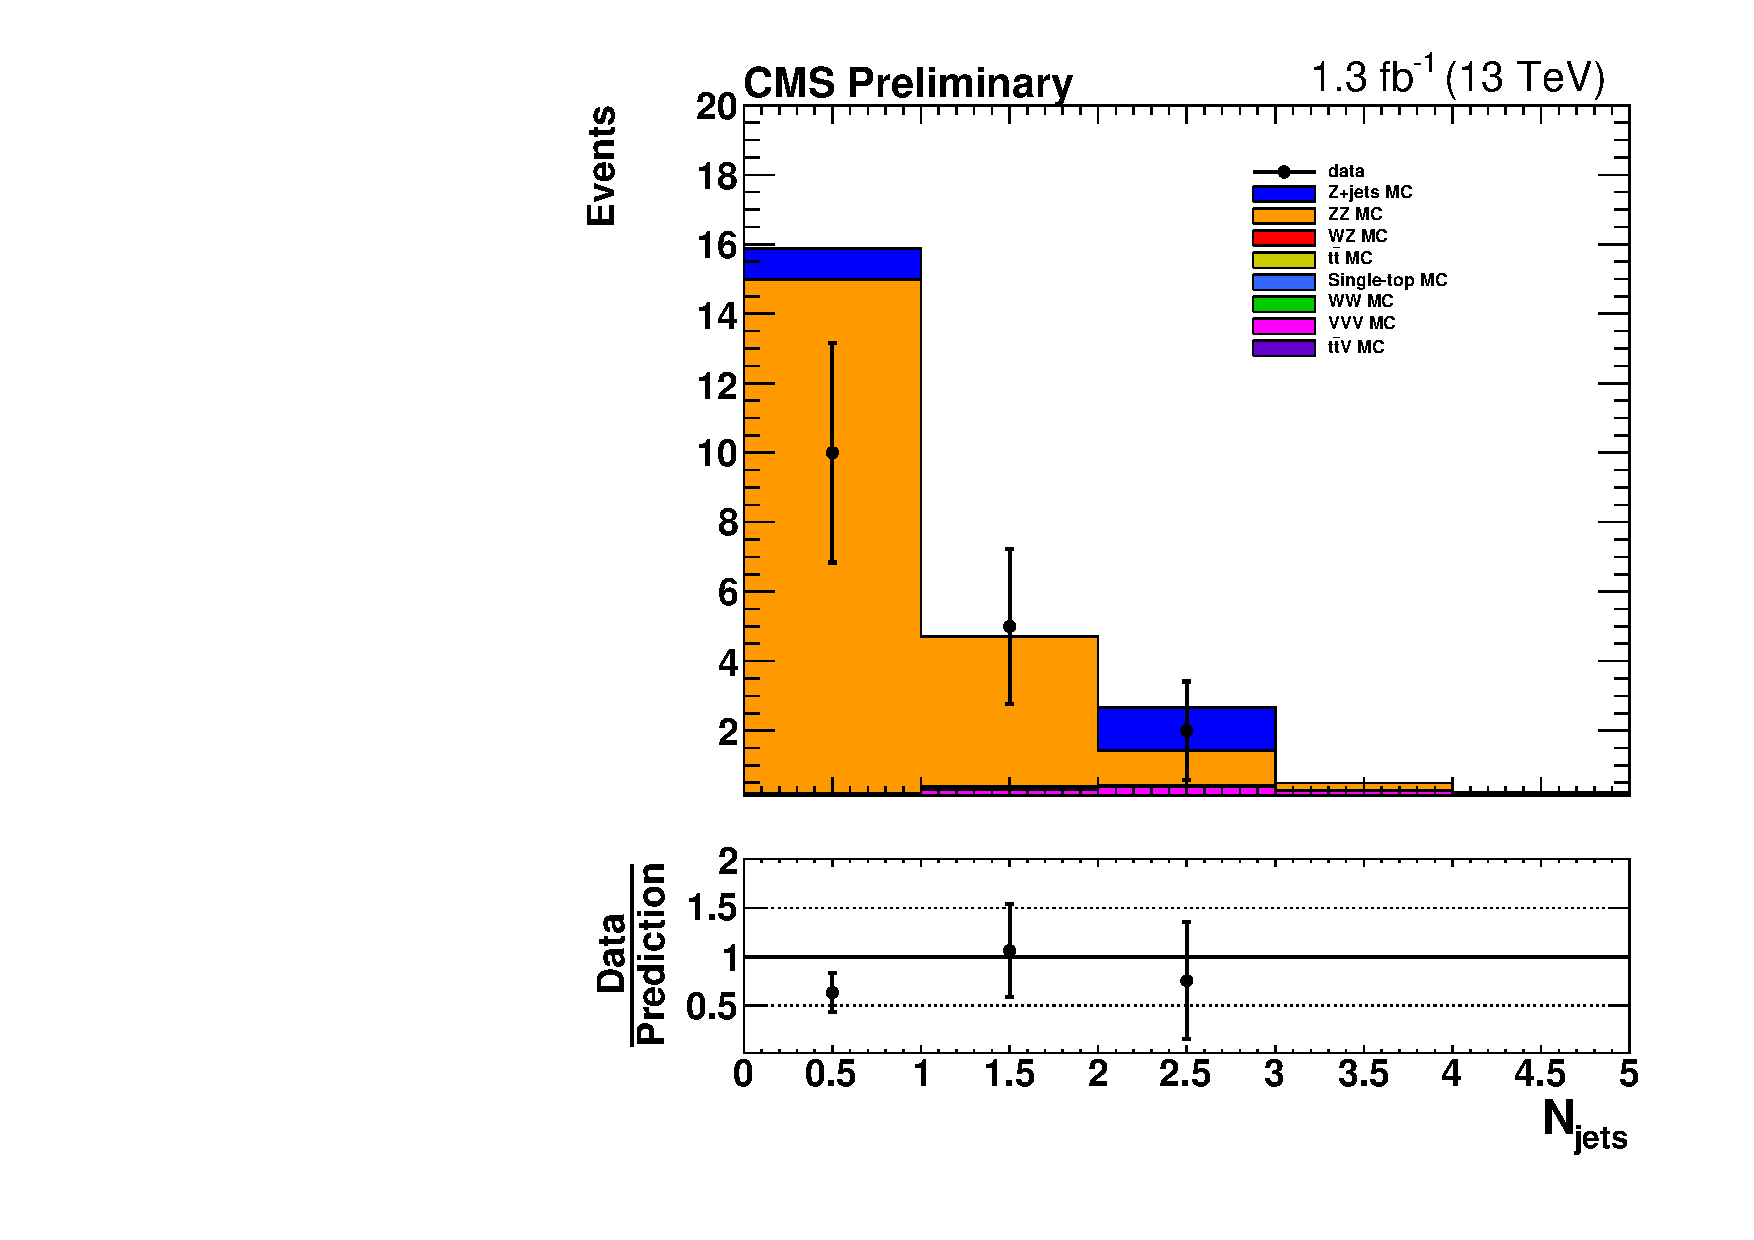
\includegraphics[width=0.4\textwidth]{bkgd/figs/h_njtall_ll_signalregion_CR4lep_passtrig.pdf} \\
\end{tabular}
\caption{The \MET\ and \nj\ distributions are shown for data vs. MC in the 4-lepton control region.
See Tables~\ref{tab:met_CR4lep}~and~\ref{tab:njets_CR4lep}~for yields.
\label{fig:bkg_CR4lep}
}
\end{center}
\end{figure}




\begin{table}[htb]
  \scriptsize
  \begin{center}
    \caption{\label{tab:met_CR4lep} 
      Yields in the 4-lepton control region binned in \MET. Uncertainties for each region are statistical only. 
    }
    \scalebox{0.8}{
      \begin{tabular}{l|c|c|c|c|c}
        \hline
        \hline
        $\mathrm{E_{T}^{miss} [GeV]}$ &0 - 10 & 10 - 20 & 20 - 30 & 30 - 40 & $\geq$ 40 \\
        \hline 
        Z+jets&  $<$ 0.1 &  1.5 $\pm$ 1.0 &  0.7 $\pm$ 0.7 &  $<$ 0.1 &  0.1 $\pm$ 0.1 \\ 
        FS bkg&  $<$ 0.1 &  $<$ 0.1 &  $<$ 0.1 &  $<$ 0.1 &  0.1 $\pm$ 0.0 \\ 
        WZ + ZZ bkg&  3.1 $\pm$ 0.0 &  6.3 $\pm$ 0.1 &  5.4 $\pm$ 0.1 &  3.1 $\pm$ 0.0 &  2.4 $\pm$ 0.0 \\ 
        ttv SM BG&  $<$ 0.1 &  $<$ 0.1 &  $<$ 0.1 &  $<$ 0.1 &  0.2 $\pm$ 0.0 \\ 
        vvv SM BG&  $<$ 0.1 &  $<$ 0.1 &  $<$ 0.1 &  0.1 $\pm$ 0.0 &  0.8 $\pm$ 0.1 \\ 
        \hline 
        total BG&  3.2 $\pm$ 0.0 &  7.9 $\pm$ 1.0 &  6.1 $\pm$ 0.7 &  3.2 $\pm$ 0.0 &  3.6 $\pm$ 0.1 \\ 
        \hline 
        Data&  2 &  7 &  2 &  1 &  5 \\ 
        \hline 
        Data/BG&  0.63 $\pm$ 0.45 &  0.89 $\pm$ 0.36 &  0.33 $\pm$ 0.23 &  0.31 $\pm$ 0.31 &  1.40 $\pm$ 0.63 \\ 
        \hline
        \hline
      \end{tabular}
    }
  \end{center}
\end{table}


\begin{table}[htb]
  \scriptsize
  \begin{center}
    \caption{\label{tab:njets_CR4lep} 
      Yields in the 4-lepton control region split by \nj. Uncertainties for each region are statistical only. 
    }
    \scalebox{0.8}{
      \begin{tabular}{l|c|c|c|c|c}
        \hline
        \hline
        $\mathrm{N_{jets}}$ &0  & 1  & 2  & 3  & $\geq$ 4 \\
        \hline 
        Z+jets&  0.9 $\pm$ 0.7 &  $<$ 0.1 &  1.2 $\pm$ 1.0 &  $<$ 0.1 &  0.1 $\pm$ 0.1 \\ 
        FS bkg&  $<$ 0.1 &  0.1 $\pm$ 0.0 &  $<$ 0.1 &  $<$ 0.1 &  $<$ 0.1 \\ 
        WZ + ZZ bkg&  14.8 $\pm$ 0.1 &  4.3 $\pm$ 0.0 &  1.0 $\pm$ 0.0 &  0.2 $\pm$ 0.0 &  $<$ 0.1 \\ 
        ttv SM BG&  0.1 $\pm$ 0.0 &  0.1 $\pm$ 0.0 &  $<$ 0.1 &  $<$ 0.1 &  $<$ 0.1 \\ 
        vvv SM BG&  $<$ 0.1 &  0.2 $\pm$ 0.0 &  0.3 $\pm$ 0.0 &  0.3 $\pm$ 0.0 &  0.1 $\pm$ 0.0 \\ 
        \hline 
        total BG&  15.9 $\pm$ 0.7 &  4.7 $\pm$ 0.1 &  2.7 $\pm$ 1.0 &  0.5 $\pm$ 0.0 &  0.2 $\pm$ 0.1 \\ 
        \hline 
        Data&  10 &  5 &  2 &  0 &  0 \\ 
        \hline 
        Data/BG&  0.63 $\pm$ 0.20 &  1.06 $\pm$ 0.47 &  0.75 $\pm$ 0.60 &  -- &  -- \\ 
        \hline
        \hline
      \end{tabular}
    }
  \end{center}
\end{table}

\clearpage
